\documentclass[twoside]{book}

% Packages required by doxygen
\usepackage{fixltx2e}
\usepackage{calc}
\usepackage{doxygen}
\usepackage[export]{adjustbox} % also loads graphicx
\usepackage{graphicx}
\usepackage[utf8]{inputenc}
\usepackage{makeidx}
\usepackage{multicol}
\usepackage{multirow}
\PassOptionsToPackage{warn}{textcomp}
\usepackage{textcomp}
\usepackage[nointegrals]{wasysym}
\usepackage[table]{xcolor}

% Font selection
\usepackage[T1]{fontenc}
\usepackage[scaled=.90]{helvet}
\usepackage{courier}
\usepackage{amssymb}
\usepackage{sectsty}
\renewcommand{\familydefault}{\sfdefault}
\allsectionsfont{%
  \fontseries{bc}\selectfont%
  \color{darkgray}%
}
\renewcommand{\DoxyLabelFont}{%
  \fontseries{bc}\selectfont%
  \color{darkgray}%
}
\newcommand{\+}{\discretionary{\mbox{\scriptsize$\hookleftarrow$}}{}{}}

% Page & text layout
\usepackage{geometry}
\geometry{%
  a4paper,%
  top=2.5cm,%
  bottom=2.5cm,%
  left=2.5cm,%
  right=2.5cm%
}
\tolerance=750
\hfuzz=15pt
\hbadness=750
\setlength{\emergencystretch}{15pt}
\setlength{\parindent}{0cm}
\setlength{\parskip}{3ex plus 2ex minus 2ex}
\makeatletter
\renewcommand{\paragraph}{%
  \@startsection{paragraph}{4}{0ex}{-1.0ex}{1.0ex}{%
    \normalfont\normalsize\bfseries\SS@parafont%
  }%
}
\renewcommand{\subparagraph}{%
  \@startsection{subparagraph}{5}{0ex}{-1.0ex}{1.0ex}{%
    \normalfont\normalsize\bfseries\SS@subparafont%
  }%
}
\makeatother

% Headers & footers
\usepackage{fancyhdr}
\pagestyle{fancyplain}
\fancyhead[LE]{\fancyplain{}{\bfseries\thepage}}
\fancyhead[CE]{\fancyplain{}{}}
\fancyhead[RE]{\fancyplain{}{\bfseries\leftmark}}
\fancyhead[LO]{\fancyplain{}{\bfseries\rightmark}}
\fancyhead[CO]{\fancyplain{}{}}
\fancyhead[RO]{\fancyplain{}{\bfseries\thepage}}
\fancyfoot[LE]{\fancyplain{}{}}
\fancyfoot[CE]{\fancyplain{}{}}
\fancyfoot[RE]{\fancyplain{}{\bfseries\scriptsize Generated by Doxygen }}
\fancyfoot[LO]{\fancyplain{}{\bfseries\scriptsize Generated by Doxygen }}
\fancyfoot[CO]{\fancyplain{}{}}
\fancyfoot[RO]{\fancyplain{}{}}
\renewcommand{\footrulewidth}{0.4pt}
\renewcommand{\chaptermark}[1]{%
  \markboth{#1}{}%
}
\renewcommand{\sectionmark}[1]{%
  \markright{\thesection\ #1}%
}

% Indices & bibliography
\usepackage{natbib}
\usepackage[titles]{tocloft}
\setcounter{tocdepth}{3}
\setcounter{secnumdepth}{5}
\makeindex

% Hyperlinks (required, but should be loaded last)
\usepackage{ifpdf}
\ifpdf
  \usepackage[pdftex,pagebackref=true]{hyperref}
\else
  \usepackage[ps2pdf,pagebackref=true]{hyperref}
\fi
\hypersetup{%
  colorlinks=true,%
  linkcolor=blue,%
  citecolor=blue,%
  unicode%
}

% Custom commands
\newcommand{\clearemptydoublepage}{%
  \newpage{\pagestyle{empty}\cleardoublepage}%
}

\usepackage{caption}
\captionsetup{labelsep=space,justification=centering,font={bf},singlelinecheck=off,skip=4pt,position=top}

%===== C O N T E N T S =====

\begin{document}

% Titlepage & ToC
\hypersetup{pageanchor=false,
             bookmarksnumbered=true,
             pdfencoding=unicode
            }
\pagenumbering{alph}
\begin{titlepage}
\vspace*{7cm}
\begin{center}%
{\Large Spectrum \\[1ex]\large 0.\+3 }\\
\vspace*{1cm}
{\large Generated by Doxygen 1.8.12}\\
\end{center}
\end{titlepage}
\clearemptydoublepage
\pagenumbering{roman}
\tableofcontents
\clearemptydoublepage
\pagenumbering{arabic}
\hypersetup{pageanchor=true}

%--- Begin generated contents ---
\chapter{Namespace Index}
\section{Namespace List}
Here is a list of all namespaces with brief descriptions\+:\begin{DoxyCompactList}
\item\contentsline{section}{\hyperlink{namespace_ui}{Ui} }{\pageref{namespace_ui}}{}
\end{DoxyCompactList}

\chapter{Hierarchical Index}
\section{Class Hierarchy}
This inheritance list is sorted roughly, but not completely, alphabetically\+:\begin{DoxyCompactList}
\item \contentsline{section}{chunk}{\pageref{structchunk}}{}
\item \contentsline{section}{Combined\+Header}{\pageref{struct_combined_header}}{}
\item \contentsline{section}{D\+A\+T\+A\+Header}{\pageref{struct_d_a_t_a_header}}{}
\item \contentsline{section}{Frequency\+Spectrum\+:\+:Element}{\pageref{struct_frequency_spectrum_1_1_element}}{}
\item \contentsline{section}{Frequency\+Spectrum}{\pageref{class_frequency_spectrum}}{}
\item \contentsline{section}{Null\+Debug}{\pageref{class_null_debug}}{}
\item \contentsline{section}{Power\+Of\+Two$<$ N $>$}{\pageref{class_power_of_two}}{}
\item \contentsline{section}{Power\+Of\+Two$<$ 0 $>$}{\pageref{class_power_of_two_3_010_01_4}}{}
\item Q\+Dialog\begin{DoxyCompactList}
\item \contentsline{section}{Settings\+Dialog}{\pageref{class_settings_dialog}}{}
\end{DoxyCompactList}
\item Q\+File\begin{DoxyCompactList}
\item \contentsline{section}{Wav\+File}{\pageref{class_wav_file}}{}
\end{DoxyCompactList}
\item Q\+Main\+Window\begin{DoxyCompactList}
\item \contentsline{section}{Main\+Widget}{\pageref{class_main_widget}}{}
\end{DoxyCompactList}
\item Q\+Object\begin{DoxyCompactList}
\item \contentsline{section}{Engine}{\pageref{class_engine}}{}
\item \contentsline{section}{Filter}{\pageref{class_filter}}{}
\begin{DoxyCompactList}
\item \contentsline{section}{Custom\+Filter}{\pageref{class_custom_filter}}{}
\item \contentsline{section}{Null\+Filter}{\pageref{class_null_filter}}{}
\end{DoxyCompactList}
\item \contentsline{section}{Graph}{\pageref{class_graph}}{}
\item \contentsline{section}{Graph\+Filter\+Service}{\pageref{class_graph_filter_service}}{}
\item \contentsline{section}{Level\+Meter}{\pageref{class_level_meter}}{}
\item \contentsline{section}{Progress\+Bar}{\pageref{class_progress_bar}}{}
\item \contentsline{section}{Spectrograph}{\pageref{class_spectrograph}}{}
\item \contentsline{section}{Spectrum\+Analyser}{\pageref{class_spectrum_analyser}}{}
\item \contentsline{section}{Spectrum\+Analyser\+Thread}{\pageref{class_spectrum_analyser_thread}}{}
\item \contentsline{section}{Wave\+Form\+Custom}{\pageref{class_wave_form_custom}}{}
\end{DoxyCompactList}
\item Q\+Widget\begin{DoxyCompactList}
\item \contentsline{section}{Waveform}{\pageref{class_waveform}}{}
\end{DoxyCompactList}
\item \contentsline{section}{R\+I\+F\+F\+Header}{\pageref{struct_r_i_f_f_header}}{}
\item \contentsline{section}{Series\+Chanel}{\pageref{struct_series_chanel}}{}
\item \contentsline{section}{Swept\+Tone}{\pageref{struct_swept_tone}}{}
\item \contentsline{section}{Tone}{\pageref{struct_tone}}{}
\item \contentsline{section}{W\+A\+V\+E\+Header}{\pageref{struct_w_a_v_e_header}}{}
\end{DoxyCompactList}

\chapter{Class Index}
\section{Class List}
Here are the classes, structs, unions and interfaces with brief descriptions\+:\begin{DoxyCompactList}
\item\contentsline{section}{\hyperlink{structchunk}{chunk} }{\pageref{structchunk}}{}
\item\contentsline{section}{\hyperlink{struct_combined_header}{Combined\+Header} }{\pageref{struct_combined_header}}{}
\item\contentsline{section}{\hyperlink{class_custom_filter}{Custom\+Filter} \\*Simple filter type. which can use an array of input dividers for filtering }{\pageref{class_custom_filter}}{}
\item\contentsline{section}{\hyperlink{struct_d_a_t_a_header}{D\+A\+T\+A\+Header} }{\pageref{struct_d_a_t_a_header}}{}
\item\contentsline{section}{\hyperlink{struct_frequency_spectrum_1_1_element}{Frequency\+Spectrum\+::\+Element} }{\pageref{struct_frequency_spectrum_1_1_element}}{}
\item\contentsline{section}{\hyperlink{class_engine}{Engine} }{\pageref{class_engine}}{}
\item\contentsline{section}{\hyperlink{class_filter}{Filter} \\*The \hyperlink{class_filter}{Filter} class  abstract vision of filter }{\pageref{class_filter}}{}
\item\contentsline{section}{\hyperlink{class_frequency_spectrum}{Frequency\+Spectrum} }{\pageref{class_frequency_spectrum}}{}
\item\contentsline{section}{\hyperlink{class_graph}{Graph} }{\pageref{class_graph}}{}
\item\contentsline{section}{\hyperlink{class_graph_filter_service}{Graph\+Filter\+Service} \\*The \hyperlink{class_graph_filter_service}{Graph\+Filter\+Service} class This class acts as an intermediate element between the user interface and classes for charts }{\pageref{class_graph_filter_service}}{}
\item\contentsline{section}{\hyperlink{class_level_meter}{Level\+Meter} }{\pageref{class_level_meter}}{}
\item\contentsline{section}{\hyperlink{class_main_widget}{Main\+Widget} }{\pageref{class_main_widget}}{}
\item\contentsline{section}{\hyperlink{class_null_debug}{Null\+Debug} }{\pageref{class_null_debug}}{}
\item\contentsline{section}{\hyperlink{class_null_filter}{Null\+Filter} \\*The \hyperlink{class_null_filter}{Null\+Filter} class }{\pageref{class_null_filter}}{}
\item\contentsline{section}{\hyperlink{class_power_of_two}{Power\+Of\+Two$<$ N $>$} }{\pageref{class_power_of_two}}{}
\item\contentsline{section}{\hyperlink{class_power_of_two_3_010_01_4}{Power\+Of\+Two$<$ 0 $>$} }{\pageref{class_power_of_two_3_010_01_4}}{}
\item\contentsline{section}{\hyperlink{class_progress_bar}{Progress\+Bar} }{\pageref{class_progress_bar}}{}
\item\contentsline{section}{\hyperlink{struct_r_i_f_f_header}{R\+I\+F\+F\+Header} }{\pageref{struct_r_i_f_f_header}}{}
\item\contentsline{section}{\hyperlink{struct_series_chanel}{Series\+Chanel} }{\pageref{struct_series_chanel}}{}
\item\contentsline{section}{\hyperlink{class_settings_dialog}{Settings\+Dialog} }{\pageref{class_settings_dialog}}{}
\item\contentsline{section}{\hyperlink{class_spectrograph}{Spectrograph} }{\pageref{class_spectrograph}}{}
\item\contentsline{section}{\hyperlink{class_spectrum_analyser}{Spectrum\+Analyser} }{\pageref{class_spectrum_analyser}}{}
\item\contentsline{section}{\hyperlink{class_spectrum_analyser_thread}{Spectrum\+Analyser\+Thread} }{\pageref{class_spectrum_analyser_thread}}{}
\item\contentsline{section}{\hyperlink{struct_swept_tone}{Swept\+Tone} }{\pageref{struct_swept_tone}}{}
\item\contentsline{section}{\hyperlink{struct_tone}{Tone} }{\pageref{struct_tone}}{}
\item\contentsline{section}{\hyperlink{class_waveform}{Waveform} }{\pageref{class_waveform}}{}
\item\contentsline{section}{\hyperlink{class_wave_form_custom}{Wave\+Form\+Custom} }{\pageref{class_wave_form_custom}}{}
\item\contentsline{section}{\hyperlink{struct_w_a_v_e_header}{W\+A\+V\+E\+Header} }{\pageref{struct_w_a_v_e_header}}{}
\item\contentsline{section}{\hyperlink{class_wav_file}{Wav\+File} \\*The \hyperlink{class_wav_file}{Wav\+File} class Simple wraper to wav file }{\pageref{class_wav_file}}{}
\end{DoxyCompactList}

\chapter{File Index}
\section{File List}
Here is a list of all files with brief descriptions\+:\begin{DoxyCompactList}
\item\contentsline{section}{app/\hyperlink{customfilter_8cpp}{customfilter.\+cpp} }{\pageref{customfilter_8cpp}}{}
\item\contentsline{section}{app/\hyperlink{customfilter_8h}{customfilter.\+h} }{\pageref{customfilter_8h}}{}
\item\contentsline{section}{app/\hyperlink{datasource_8cpp}{datasource.\+cpp} }{\pageref{datasource_8cpp}}{}
\item\contentsline{section}{app/\hyperlink{datasource_8h}{datasource.\+h} }{\pageref{datasource_8h}}{}
\item\contentsline{section}{app/\hyperlink{engine_8cpp}{engine.\+cpp} }{\pageref{engine_8cpp}}{}
\item\contentsline{section}{app/\hyperlink{engine_8h}{engine.\+h} }{\pageref{engine_8h}}{}
\item\contentsline{section}{app/\hyperlink{filter_8cpp}{filter.\+cpp} }{\pageref{filter_8cpp}}{}
\item\contentsline{section}{app/\hyperlink{filter_8h}{filter.\+h} }{\pageref{filter_8h}}{}
\item\contentsline{section}{app/\hyperlink{frequencyspectrum_8cpp}{frequencyspectrum.\+cpp} }{\pageref{frequencyspectrum_8cpp}}{}
\item\contentsline{section}{app/\hyperlink{frequencyspectrum_8h}{frequencyspectrum.\+h} }{\pageref{frequencyspectrum_8h}}{}
\item\contentsline{section}{app/\hyperlink{graph_8cpp}{graph.\+cpp} }{\pageref{graph_8cpp}}{}
\item\contentsline{section}{app/\hyperlink{graph_8h}{graph.\+h} }{\pageref{graph_8h}}{}
\item\contentsline{section}{app/\hyperlink{graphfilterservice_8cpp}{graphfilterservice.\+cpp} }{\pageref{graphfilterservice_8cpp}}{}
\item\contentsline{section}{app/\hyperlink{graphfilterservice_8h}{graphfilterservice.\+h} }{\pageref{graphfilterservice_8h}}{}
\item\contentsline{section}{app/\hyperlink{levelmeter_8cpp}{levelmeter.\+cpp} }{\pageref{levelmeter_8cpp}}{}
\item\contentsline{section}{app/\hyperlink{levelmeter_8h}{levelmeter.\+h} }{\pageref{levelmeter_8h}}{}
\item\contentsline{section}{app/\hyperlink{main_8cpp}{main.\+cpp} }{\pageref{main_8cpp}}{}
\item\contentsline{section}{app/\hyperlink{mainwidget_8cpp}{mainwidget.\+cpp} }{\pageref{mainwidget_8cpp}}{}
\item\contentsline{section}{app/\hyperlink{mainwidget_8h}{mainwidget.\+h} }{\pageref{mainwidget_8h}}{}
\item\contentsline{section}{app/\hyperlink{nullfilter_8cpp}{nullfilter.\+cpp} }{\pageref{nullfilter_8cpp}}{}
\item\contentsline{section}{app/\hyperlink{nullfilter_8h}{nullfilter.\+h} }{\pageref{nullfilter_8h}}{}
\item\contentsline{section}{app/\hyperlink{progressbar_8cpp}{progressbar.\+cpp} }{\pageref{progressbar_8cpp}}{}
\item\contentsline{section}{app/\hyperlink{progressbar_8h}{progressbar.\+h} }{\pageref{progressbar_8h}}{}
\item\contentsline{section}{app/\hyperlink{settingsdialog_8cpp}{settingsdialog.\+cpp} }{\pageref{settingsdialog_8cpp}}{}
\item\contentsline{section}{app/\hyperlink{settingsdialog_8h}{settingsdialog.\+h} }{\pageref{settingsdialog_8h}}{}
\item\contentsline{section}{app/\hyperlink{spectrograph_8cpp}{spectrograph.\+cpp} }{\pageref{spectrograph_8cpp}}{}
\item\contentsline{section}{app/\hyperlink{spectrograph_8h}{spectrograph.\+h} }{\pageref{spectrograph_8h}}{}
\item\contentsline{section}{app/\hyperlink{spectrum_8h}{spectrum.\+h} }{\pageref{spectrum_8h}}{}
\item\contentsline{section}{app/\hyperlink{spectrumanalyser_8cpp}{spectrumanalyser.\+cpp} }{\pageref{spectrumanalyser_8cpp}}{}
\item\contentsline{section}{app/\hyperlink{spectrumanalyser_8h}{spectrumanalyser.\+h} }{\pageref{spectrumanalyser_8h}}{}
\item\contentsline{section}{app/\hyperlink{utils_8cpp}{utils.\+cpp} }{\pageref{utils_8cpp}}{}
\item\contentsline{section}{app/\hyperlink{utils_8h}{utils.\+h} }{\pageref{utils_8h}}{}
\item\contentsline{section}{app/\hyperlink{waveform_8cpp}{waveform.\+cpp} }{\pageref{waveform_8cpp}}{}
\item\contentsline{section}{app/\hyperlink{waveform_8h}{waveform.\+h} }{\pageref{waveform_8h}}{}
\item\contentsline{section}{app/\hyperlink{wavfile_8cpp}{wavfile.\+cpp} }{\pageref{wavfile_8cpp}}{}
\item\contentsline{section}{app/\hyperlink{wavfile_8h}{wavfile.\+h} }{\pageref{wavfile_8h}}{}
\end{DoxyCompactList}

\chapter{Namespace Documentation}
\hypertarget{namespace_ui}{}\section{Ui Namespace Reference}
\label{namespace_ui}\index{Ui@{Ui}}

\chapter{Class Documentation}
\hypertarget{structchunk}{}\section{chunk Struct Reference}
\label{structchunk}\index{chunk@{chunk}}
\subsection*{Public Attributes}
\begin{DoxyCompactItemize}
\item 
char \hyperlink{structchunk_abbdb8d8e521edcb7483320c66526d34e}{id} \mbox{[}4\mbox{]}
\item 
quint32 \hyperlink{structchunk_a93de60bdeb204f9b7572c346584ce680}{size}
\end{DoxyCompactItemize}


\subsection{Member Data Documentation}
\hypertarget{structchunk_abbdb8d8e521edcb7483320c66526d34e}{}\label{structchunk_abbdb8d8e521edcb7483320c66526d34e} 
\index{chunk@{chunk}!id@{id}}
\index{id@{id}!chunk@{chunk}}
\subsubsection{\texorpdfstring{id}{id}}
{\footnotesize\ttfamily char chunk\+::id\mbox{[}4\mbox{]}}

\hypertarget{structchunk_a93de60bdeb204f9b7572c346584ce680}{}\label{structchunk_a93de60bdeb204f9b7572c346584ce680} 
\index{chunk@{chunk}!size@{size}}
\index{size@{size}!chunk@{chunk}}
\subsubsection{\texorpdfstring{size}{size}}
{\footnotesize\ttfamily quint32 chunk\+::size}



The documentation for this struct was generated from the following file\+:\begin{DoxyCompactItemize}
\item 
app/\hyperlink{wavfile_8cpp}{wavfile.\+cpp}\end{DoxyCompactItemize}

\hypertarget{struct_combined_header}{}\section{Combined\+Header Struct Reference}
\label{struct_combined_header}\index{Combined\+Header@{Combined\+Header}}
\subsection*{Public Attributes}
\begin{DoxyCompactItemize}
\item 
\hyperlink{struct_r_i_f_f_header}{R\+I\+F\+F\+Header} \hyperlink{struct_combined_header_ad31d827b36c88f885c9a0a4616414056}{riff}
\item 
\hyperlink{struct_w_a_v_e_header}{W\+A\+V\+E\+Header} \hyperlink{struct_combined_header_aa74e3cc8011eac683c9b1ae366a6cc6a}{wave}
\end{DoxyCompactItemize}


\subsection{Member Data Documentation}
\hypertarget{struct_combined_header_ad31d827b36c88f885c9a0a4616414056}{}\label{struct_combined_header_ad31d827b36c88f885c9a0a4616414056} 
\index{Combined\+Header@{Combined\+Header}!riff@{riff}}
\index{riff@{riff}!Combined\+Header@{Combined\+Header}}
\subsubsection{\texorpdfstring{riff}{riff}}
{\footnotesize\ttfamily \hyperlink{struct_r_i_f_f_header}{R\+I\+F\+F\+Header} Combined\+Header\+::riff}

\hypertarget{struct_combined_header_aa74e3cc8011eac683c9b1ae366a6cc6a}{}\label{struct_combined_header_aa74e3cc8011eac683c9b1ae366a6cc6a} 
\index{Combined\+Header@{Combined\+Header}!wave@{wave}}
\index{wave@{wave}!Combined\+Header@{Combined\+Header}}
\subsubsection{\texorpdfstring{wave}{wave}}
{\footnotesize\ttfamily \hyperlink{struct_w_a_v_e_header}{W\+A\+V\+E\+Header} Combined\+Header\+::wave}



The documentation for this struct was generated from the following file\+:\begin{DoxyCompactItemize}
\item 
app/\hyperlink{wavfile_8cpp}{wavfile.\+cpp}\end{DoxyCompactItemize}

\hypertarget{class_custom_filter}{}\section{Custom\+Filter Class Reference}
\label{class_custom_filter}\index{Custom\+Filter@{Custom\+Filter}}


Simple filter type. which can use an array of input dividers for filtering.  




{\ttfamily \#include $<$customfilter.\+h$>$}

Inheritance diagram for Custom\+Filter\+:\begin{figure}[H]
\begin{center}
\leavevmode
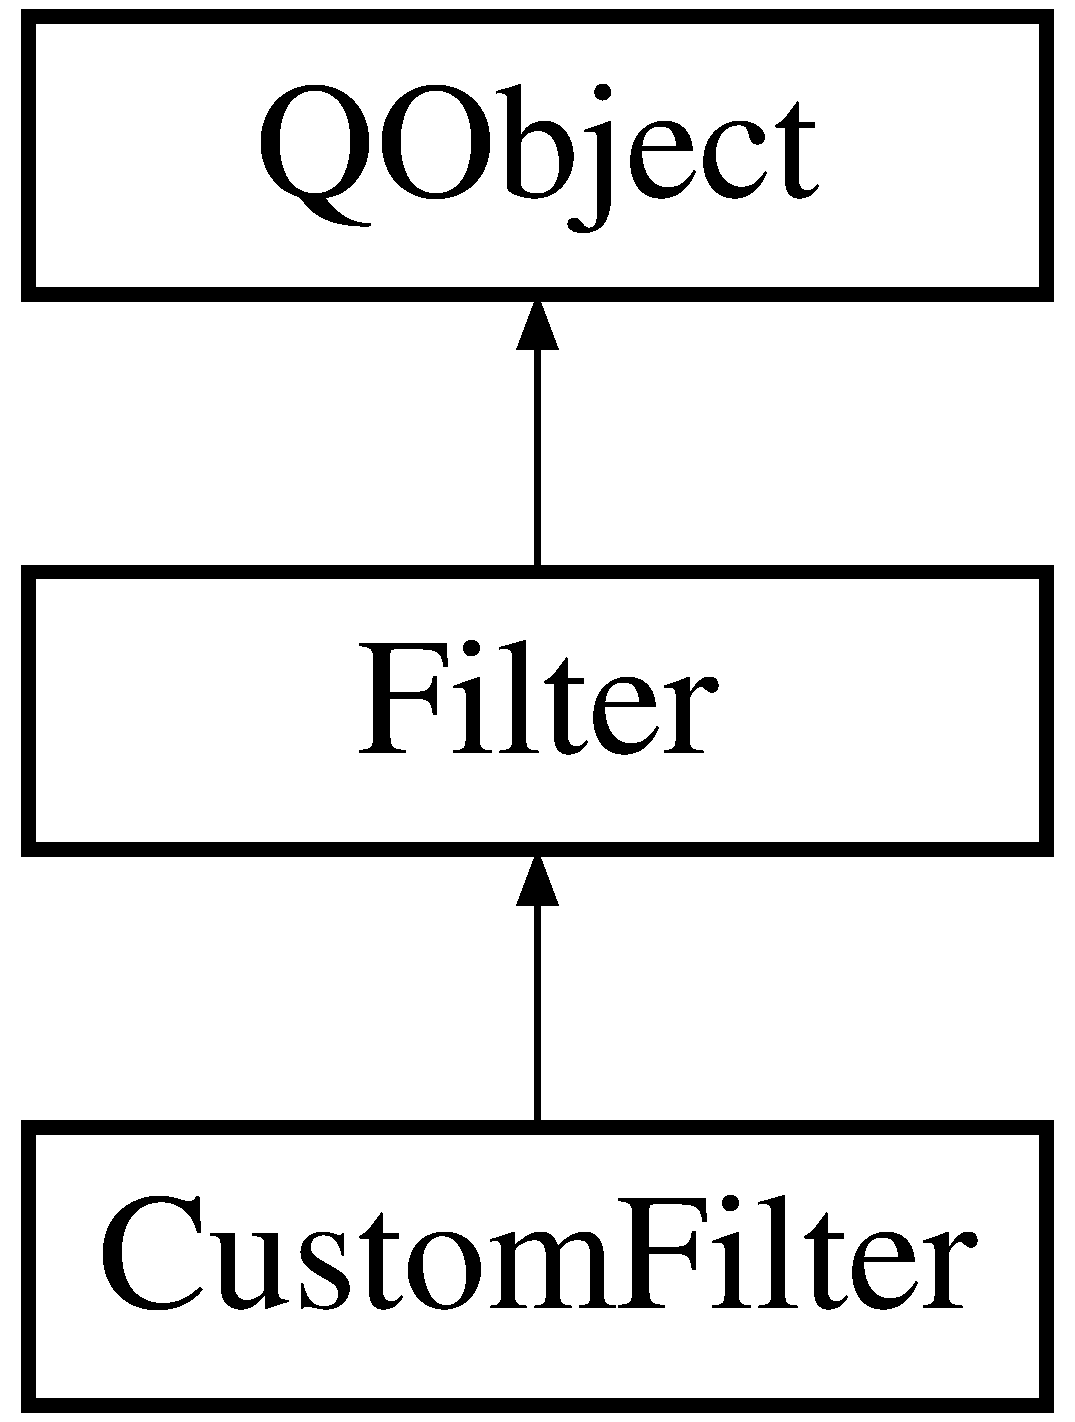
\includegraphics[height=3.000000cm]{class_custom_filter}
\end{center}
\end{figure}
\subsection*{Public Member Functions}
\begin{DoxyCompactItemize}
\item 
\hyperlink{class_custom_filter_aea563fa1531896e1e6427c42e8694ecf}{Custom\+Filter} (Q\+List$<$ float $>$ params, Q\+Object $\ast$parent=0)
\begin{DoxyCompactList}\small\item\em \hyperlink{class_custom_filter}{Custom\+Filter} constuctor. \end{DoxyCompactList}\item 
Q\+Byte\+Array \hyperlink{class_custom_filter_aafa4ccbab26275b5ef223158cbb684ab}{do\+Filter} (Q\+Audio\+Format format, Q\+Byte\+Array array)
\begin{DoxyCompactList}\small\item\em do\+Filter \end{DoxyCompactList}\end{DoxyCompactItemize}


\subsection{Detailed Description}
Simple filter type. which can use an array of input dividers for filtering. 

\subsection{Constructor \& Destructor Documentation}
\hypertarget{class_custom_filter_aea563fa1531896e1e6427c42e8694ecf}{}\label{class_custom_filter_aea563fa1531896e1e6427c42e8694ecf} 
\index{Custom\+Filter@{Custom\+Filter}!Custom\+Filter@{Custom\+Filter}}
\index{Custom\+Filter@{Custom\+Filter}!Custom\+Filter@{Custom\+Filter}}
\subsubsection{\texorpdfstring{Custom\+Filter()}{CustomFilter()}}
{\footnotesize\ttfamily Custom\+Filter\+::\+Custom\+Filter (\begin{DoxyParamCaption}\item[{Q\+List$<$ float $>$}]{params,  }\item[{Q\+Object $\ast$}]{parent = {\ttfamily 0} }\end{DoxyParamCaption})}



\hyperlink{class_custom_filter}{Custom\+Filter} constuctor. 


\begin{DoxyParams}{Parameters}
{\em params} & -\/ array of divider which use for filtering \\
\hline
{\em parent} & -\/ parent object (only for CC) \\
\hline
\end{DoxyParams}


\subsection{Member Function Documentation}
\hypertarget{class_custom_filter_aafa4ccbab26275b5ef223158cbb684ab}{}\label{class_custom_filter_aafa4ccbab26275b5ef223158cbb684ab} 
\index{Custom\+Filter@{Custom\+Filter}!do\+Filter@{do\+Filter}}
\index{do\+Filter@{do\+Filter}!Custom\+Filter@{Custom\+Filter}}
\subsubsection{\texorpdfstring{do\+Filter()}{doFilter()}}
{\footnotesize\ttfamily Q\+Byte\+Array Custom\+Filter\+::do\+Filter (\begin{DoxyParamCaption}\item[{Q\+Audio\+Format}]{format,  }\item[{Q\+Byte\+Array}]{array }\end{DoxyParamCaption})\hspace{0.3cm}{\ttfamily [virtual]}}



do\+Filter 


\begin{DoxyParams}{Parameters}
{\em format} & -\/ audio format \\
\hline
{\em array} & -\/ input data for filtering \\
\hline
\end{DoxyParams}
\begin{DoxyReturn}{Returns}
well done filtered buffer 
\end{DoxyReturn}


Implements \hyperlink{class_filter_aa401218a142d916f84aafece09eac301}{Filter}.



The documentation for this class was generated from the following files\+:\begin{DoxyCompactItemize}
\item 
app/\hyperlink{customfilter_8h}{customfilter.\+h}\item 
app/\hyperlink{customfilter_8cpp}{customfilter.\+cpp}\end{DoxyCompactItemize}

\hypertarget{struct_d_a_t_a_header}{}\section{D\+A\+T\+A\+Header Struct Reference}
\label{struct_d_a_t_a_header}\index{D\+A\+T\+A\+Header@{D\+A\+T\+A\+Header}}
\subsection*{Public Attributes}
\begin{DoxyCompactItemize}
\item 
\hyperlink{structchunk}{chunk} \hyperlink{struct_d_a_t_a_header_a27ddfe658a290eea9ef7bd6425f54585}{descriptor}
\end{DoxyCompactItemize}


\subsection{Member Data Documentation}
\hypertarget{struct_d_a_t_a_header_a27ddfe658a290eea9ef7bd6425f54585}{}\label{struct_d_a_t_a_header_a27ddfe658a290eea9ef7bd6425f54585} 
\index{D\+A\+T\+A\+Header@{D\+A\+T\+A\+Header}!descriptor@{descriptor}}
\index{descriptor@{descriptor}!D\+A\+T\+A\+Header@{D\+A\+T\+A\+Header}}
\subsubsection{\texorpdfstring{descriptor}{descriptor}}
{\footnotesize\ttfamily \hyperlink{structchunk}{chunk} D\+A\+T\+A\+Header\+::descriptor}



The documentation for this struct was generated from the following file\+:\begin{DoxyCompactItemize}
\item 
app/\hyperlink{wavfile_8cpp}{wavfile.\+cpp}\end{DoxyCompactItemize}

\hypertarget{struct_frequency_spectrum_1_1_element}{}\section{Frequency\+Spectrum\+:\+:Element Struct Reference}
\label{struct_frequency_spectrum_1_1_element}\index{Frequency\+Spectrum\+::\+Element@{Frequency\+Spectrum\+::\+Element}}


{\ttfamily \#include $<$frequencyspectrum.\+h$>$}

\subsection*{Public Member Functions}
\begin{DoxyCompactItemize}
\item 
\hyperlink{struct_frequency_spectrum_1_1_element_a60e974e83dfd98518339e2681d8cdcdc}{Element} ()
\end{DoxyCompactItemize}
\subsection*{Public Attributes}
\begin{DoxyCompactItemize}
\item 
qreal \hyperlink{struct_frequency_spectrum_1_1_element_af6fb6c8a356fc27881bca9af0b89d88f}{frequency}
\item 
qreal \hyperlink{struct_frequency_spectrum_1_1_element_a057906284c20696169f327cae2f9ca80}{amplitude}
\item 
qreal \hyperlink{struct_frequency_spectrum_1_1_element_aea3fc976c7f3ba3d916d8017d847b011}{phase}
\item 
bool \hyperlink{struct_frequency_spectrum_1_1_element_a686d40af2870a06fba032c480573792a}{clipped}
\end{DoxyCompactItemize}


\subsection{Constructor \& Destructor Documentation}
\hypertarget{struct_frequency_spectrum_1_1_element_a60e974e83dfd98518339e2681d8cdcdc}{}\label{struct_frequency_spectrum_1_1_element_a60e974e83dfd98518339e2681d8cdcdc} 
\index{Frequency\+Spectrum\+::\+Element@{Frequency\+Spectrum\+::\+Element}!Element@{Element}}
\index{Element@{Element}!Frequency\+Spectrum\+::\+Element@{Frequency\+Spectrum\+::\+Element}}
\subsubsection{\texorpdfstring{Element()}{Element()}}
{\footnotesize\ttfamily Frequency\+Spectrum\+::\+Element\+::\+Element (\begin{DoxyParamCaption}{ }\end{DoxyParamCaption})\hspace{0.3cm}{\ttfamily [inline]}}



\subsection{Member Data Documentation}
\hypertarget{struct_frequency_spectrum_1_1_element_a057906284c20696169f327cae2f9ca80}{}\label{struct_frequency_spectrum_1_1_element_a057906284c20696169f327cae2f9ca80} 
\index{Frequency\+Spectrum\+::\+Element@{Frequency\+Spectrum\+::\+Element}!amplitude@{amplitude}}
\index{amplitude@{amplitude}!Frequency\+Spectrum\+::\+Element@{Frequency\+Spectrum\+::\+Element}}
\subsubsection{\texorpdfstring{amplitude}{amplitude}}
{\footnotesize\ttfamily qreal Frequency\+Spectrum\+::\+Element\+::amplitude}

Amplitude in range \mbox{[}0.\+0, 1.\+0\mbox{]} \hypertarget{struct_frequency_spectrum_1_1_element_a686d40af2870a06fba032c480573792a}{}\label{struct_frequency_spectrum_1_1_element_a686d40af2870a06fba032c480573792a} 
\index{Frequency\+Spectrum\+::\+Element@{Frequency\+Spectrum\+::\+Element}!clipped@{clipped}}
\index{clipped@{clipped}!Frequency\+Spectrum\+::\+Element@{Frequency\+Spectrum\+::\+Element}}
\subsubsection{\texorpdfstring{clipped}{clipped}}
{\footnotesize\ttfamily bool Frequency\+Spectrum\+::\+Element\+::clipped}

Indicates whether value has been clipped during spectrum analysis \hypertarget{struct_frequency_spectrum_1_1_element_af6fb6c8a356fc27881bca9af0b89d88f}{}\label{struct_frequency_spectrum_1_1_element_af6fb6c8a356fc27881bca9af0b89d88f} 
\index{Frequency\+Spectrum\+::\+Element@{Frequency\+Spectrum\+::\+Element}!frequency@{frequency}}
\index{frequency@{frequency}!Frequency\+Spectrum\+::\+Element@{Frequency\+Spectrum\+::\+Element}}
\subsubsection{\texorpdfstring{frequency}{frequency}}
{\footnotesize\ttfamily qreal Frequency\+Spectrum\+::\+Element\+::frequency}

Frequency in Hertz \hypertarget{struct_frequency_spectrum_1_1_element_aea3fc976c7f3ba3d916d8017d847b011}{}\label{struct_frequency_spectrum_1_1_element_aea3fc976c7f3ba3d916d8017d847b011} 
\index{Frequency\+Spectrum\+::\+Element@{Frequency\+Spectrum\+::\+Element}!phase@{phase}}
\index{phase@{phase}!Frequency\+Spectrum\+::\+Element@{Frequency\+Spectrum\+::\+Element}}
\subsubsection{\texorpdfstring{phase}{phase}}
{\footnotesize\ttfamily qreal Frequency\+Spectrum\+::\+Element\+::phase}

Phase in range \mbox{[}0.\+0, 2$\ast$\+PI\mbox{]} 

The documentation for this struct was generated from the following file\+:\begin{DoxyCompactItemize}
\item 
app/\hyperlink{frequencyspectrum_8h}{frequencyspectrum.\+h}\end{DoxyCompactItemize}

\hypertarget{class_engine}{}\section{Engine Class Reference}
\label{class_engine}\index{Engine@{Engine}}


{\ttfamily \#include $<$engine.\+h$>$}

Inheritance diagram for Engine\+:\begin{figure}[H]
\begin{center}
\leavevmode
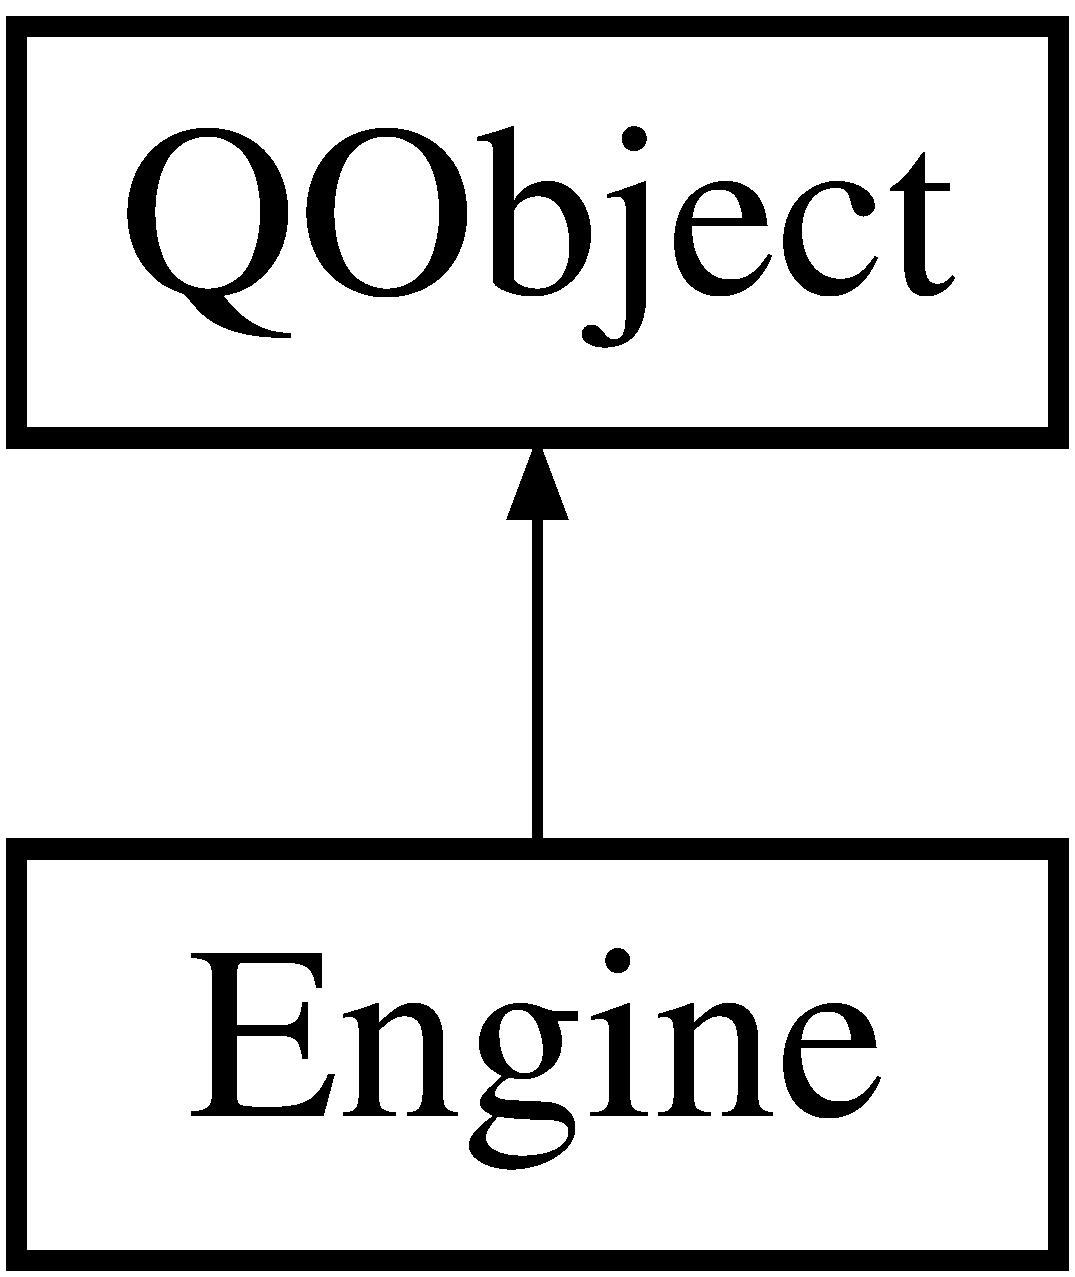
\includegraphics[height=2.000000cm]{class_engine}
\end{center}
\end{figure}
\subsection*{Public Slots}
\begin{DoxyCompactItemize}
\item 
void \hyperlink{class_engine_a642ce405fe251d783cd5766925286477}{start\+Recording} ()
\item 
void \hyperlink{class_engine_aa8314a12e4d220c5540605dd8ac3bd3a}{start\+Playback} ()
\item 
void \hyperlink{class_engine_a5a6a21b73b9571b41d45eadec6a86edd}{suspend} ()
\item 
void \hyperlink{class_engine_a382efef270e3ebe98e1b26945d080fa9}{stop\+Playback} ()
\item 
void \hyperlink{class_engine_a14fc1862412916b29b6d885d6e4865bf}{set\+Audio\+Input\+Device} (const Q\+Audio\+Device\+Info \&device)
\item 
void \hyperlink{class_engine_ae45195b977998e53441aed3006c9a35e}{set\+Audio\+Output\+Device} (const Q\+Audio\+Device\+Info \&device)
\item 
void \hyperlink{class_engine_ad36cd20d882c533e02cf6164cbc6e774}{set\+Window\+Function} (\hyperlink{spectrum_8h_adae4545e1609513867a86cc5e91fc1d4}{Window\+Function} func)
\item 
qint64 \hyperlink{class_engine_a165b8efe8055b3da607db4a6bb977a0c}{get\+Duration} ()
\item 
qint64 \hyperlink{class_engine_a9861606422c32d2dcd78ca7666f43785}{get\+Time\+Position} ()
\item 
void \hyperlink{class_engine_a52d2f257b439735853144f7cb4199f86}{set\+Time\+Position} (qint64 time)
\item 
void \hyperlink{class_engine_a56fbf122df09a4f2c7d8ef053b355459}{set\+Play\+Template} (Q\+String name)
\end{DoxyCompactItemize}
\subsection*{Signals}
\begin{DoxyCompactItemize}
\item 
void \hyperlink{class_engine_abd773c71dbe9b8433062dda03b40dc2e}{state\+Changed} (Q\+Audio\+::\+Mode \hyperlink{class_engine_a63bb47972a1e0692432dd704a60e49bc}{mode}, Q\+Audio\+::\+State \hyperlink{class_engine_af21cf755f29c026ce0bc54f392d74adc}{state})
\item 
void \hyperlink{class_engine_a8b33312dbe69efdb8f5c311439015bc3}{info\+Message} (const Q\+String \&message, int duration\+Ms)
\item 
void \hyperlink{class_engine_a15540c6090eaa691b572d89d45d72e35}{error\+Message} (const Q\+String \&heading, const Q\+String \&detail)
\item 
void \hyperlink{class_engine_a08be5a3820381f266b3bf2b3a3b91549}{format\+Changed} (const Q\+Audio\+Format \&\hyperlink{class_engine_a275e6b498d8d956e10bdeeef9c494673}{format})
\item 
void \hyperlink{class_engine_a3870ec1ab9c7ee50a8126ffb5a2dbb04}{buffer\+Length\+Changed} (qint64 duration)
\item 
void \hyperlink{class_engine_a3316fdfd7db81a74416b8180c264f361}{data\+Length\+Changed} (qint64 duration)
\item 
void \hyperlink{class_engine_ad44be9915af75cf3dab1c3a5a4665693}{record\+Position\+Changed} (qint64 position)
\item 
void \hyperlink{class_engine_afe3298aca565219a67698bf7974a5257}{play\+Position\+Changed} (qint64 position)
\item 
void \hyperlink{class_engine_acccf2905ae48b05c44e9f4ec363079ab}{level\+Changed} (qreal \hyperlink{class_engine_a0a7764981d74fab25e390fa6f91aeb03}{rms\+Level}, qreal \hyperlink{class_engine_aab1cbc9a117974fe64cb0875a02792ab}{peak\+Level}, int num\+Samples)
\item 
void \hyperlink{class_engine_a99575be39ebf22f90a48ab2c23c2d482}{spectrum\+Changed} (qint64 position, qint64 length, const \hyperlink{class_frequency_spectrum}{Frequency\+Spectrum} \&spectrum)
\item 
void \hyperlink{class_engine_a4e54e59d1adc73cce8f6d2c4457dc06d}{buffer\+Changed} (qint64 position, qint64 length, const Q\+Byte\+Array \&buffer)
\end{DoxyCompactItemize}
\subsection*{Public Member Functions}
\begin{DoxyCompactItemize}
\item 
\hyperlink{class_engine_aa9a980fee0abf2524c4c449c0894c383}{Engine} (Q\+Object $\ast$parent=0)
\item 
\hyperlink{class_engine_a8ef7030a089ecb30bbfcb9e43094717a}{$\sim$\+Engine} ()
\item 
const Q\+List$<$ Q\+Audio\+Device\+Info $>$ \& \hyperlink{class_engine_a6e06ecaa303e1b03581ce9ea296740e8}{available\+Audio\+Input\+Devices} () const
\item 
const Q\+List$<$ Q\+Audio\+Device\+Info $>$ \& \hyperlink{class_engine_a6b4c101c20dcd1843832049c379c334b}{available\+Audio\+Output\+Devices} () const
\item 
Q\+Audio\+::\+Mode \hyperlink{class_engine_a63bb47972a1e0692432dd704a60e49bc}{mode} () const
\item 
Q\+Audio\+::\+State \hyperlink{class_engine_af21cf755f29c026ce0bc54f392d74adc}{state} () const
\item 
const Q\+Audio\+Format \& \hyperlink{class_engine_a275e6b498d8d956e10bdeeef9c494673}{format} () const
\item 
void \hyperlink{class_engine_ac3b86066213c3e8a1b5186426c12bb50}{reset} ()
\item 
bool \hyperlink{class_engine_aad11dc39fb12f9ab53f9c2ec29a02aa5}{load\+File} (const Q\+String \&file\+Name)
\item 
bool \hyperlink{class_engine_aaaa5e9ce9bf266dac28460e2adaa1270}{generate\+Tone} (const \hyperlink{struct_tone}{Tone} \&tone)
\item 
bool \hyperlink{class_engine_a0fa43cb25d35f9da09b58612a8af9e77}{generate\+Swept\+Tone} (qreal amplitude)
\item 
bool \hyperlink{class_engine_a00ceb1aec88fc531e5c4decfac40b8a4}{initialize\+Record} ()
\item 
qint64 \hyperlink{class_engine_a6d176811eefe7ae0979481862670003a}{record\+Position} () const
\item 
qreal \hyperlink{class_engine_a0a7764981d74fab25e390fa6f91aeb03}{rms\+Level} () const
\item 
qreal \hyperlink{class_engine_aab1cbc9a117974fe64cb0875a02792ab}{peak\+Level} () const
\item 
qint64 \hyperlink{class_engine_a2b295fe42d3e6e4f04f56c3f63ebe945}{play\+Position} () const
\item 
qint64 \hyperlink{class_engine_a1e21c3b6d92bfa97d8ad77ce67f28264}{buffer\+Length} () const
\item 
qint64 \hyperlink{class_engine_a046bdd2d3c60411e1c08253bb1af28df}{data\+Length} () const
\item 
Q\+Map$<$ Q\+String, \hyperlink{class_graph_filter_service}{Graph\+Filter\+Service} $\ast$ $>$ \hyperlink{class_engine_a252738800567e88de862458d94bcad15}{get\+Created\+Templates} () const
\end{DoxyCompactItemize}
\subsection*{Protected Slots}
\begin{DoxyCompactItemize}
\item 
void \hyperlink{class_engine_a83047ff6af71dc546eeabccfde31d9aa}{push\+Timer\+Expired} ()
\end{DoxyCompactItemize}


\subsection{Detailed Description}
This class interfaces with the Qt Multimedia audio classes, and also with the \hyperlink{class_spectrum_analyser}{Spectrum\+Analyser} class. Its role is to manage the capture and playback of audio data, meanwhile performing real-\/time analysis of the audio level and frequency spectrum. 

\subsection{Constructor \& Destructor Documentation}
\hypertarget{class_engine_aa9a980fee0abf2524c4c449c0894c383}{}\label{class_engine_aa9a980fee0abf2524c4c449c0894c383} 
\index{Engine@{Engine}!Engine@{Engine}}
\index{Engine@{Engine}!Engine@{Engine}}
\subsubsection{\texorpdfstring{Engine()}{Engine()}}
{\footnotesize\ttfamily Engine\+::\+Engine (\begin{DoxyParamCaption}\item[{Q\+Object $\ast$}]{parent = {\ttfamily 0} }\end{DoxyParamCaption})\hspace{0.3cm}{\ttfamily [explicit]}}

\hypertarget{class_engine_a8ef7030a089ecb30bbfcb9e43094717a}{}\label{class_engine_a8ef7030a089ecb30bbfcb9e43094717a} 
\index{Engine@{Engine}!````~Engine@{$\sim$\+Engine}}
\index{````~Engine@{$\sim$\+Engine}!Engine@{Engine}}
\subsubsection{\texorpdfstring{$\sim$\+Engine()}{~Engine()}}
{\footnotesize\ttfamily Engine\+::$\sim$\+Engine (\begin{DoxyParamCaption}{ }\end{DoxyParamCaption})}



\subsection{Member Function Documentation}
\hypertarget{class_engine_a6e06ecaa303e1b03581ce9ea296740e8}{}\label{class_engine_a6e06ecaa303e1b03581ce9ea296740e8} 
\index{Engine@{Engine}!available\+Audio\+Input\+Devices@{available\+Audio\+Input\+Devices}}
\index{available\+Audio\+Input\+Devices@{available\+Audio\+Input\+Devices}!Engine@{Engine}}
\subsubsection{\texorpdfstring{available\+Audio\+Input\+Devices()}{availableAudioInputDevices()}}
{\footnotesize\ttfamily const Q\+List$<$Q\+Audio\+Device\+Info$>$\& Engine\+::available\+Audio\+Input\+Devices (\begin{DoxyParamCaption}{ }\end{DoxyParamCaption}) const\hspace{0.3cm}{\ttfamily [inline]}}

\hypertarget{class_engine_a6b4c101c20dcd1843832049c379c334b}{}\label{class_engine_a6b4c101c20dcd1843832049c379c334b} 
\index{Engine@{Engine}!available\+Audio\+Output\+Devices@{available\+Audio\+Output\+Devices}}
\index{available\+Audio\+Output\+Devices@{available\+Audio\+Output\+Devices}!Engine@{Engine}}
\subsubsection{\texorpdfstring{available\+Audio\+Output\+Devices()}{availableAudioOutputDevices()}}
{\footnotesize\ttfamily const Q\+List$<$Q\+Audio\+Device\+Info$>$\& Engine\+::available\+Audio\+Output\+Devices (\begin{DoxyParamCaption}{ }\end{DoxyParamCaption}) const\hspace{0.3cm}{\ttfamily [inline]}}

\hypertarget{class_engine_a4e54e59d1adc73cce8f6d2c4457dc06d}{}\label{class_engine_a4e54e59d1adc73cce8f6d2c4457dc06d} 
\index{Engine@{Engine}!buffer\+Changed@{buffer\+Changed}}
\index{buffer\+Changed@{buffer\+Changed}!Engine@{Engine}}
\subsubsection{\texorpdfstring{buffer\+Changed}{bufferChanged}}
{\footnotesize\ttfamily void Engine\+::buffer\+Changed (\begin{DoxyParamCaption}\item[{qint64}]{position,  }\item[{qint64}]{length,  }\item[{const Q\+Byte\+Array \&}]{buffer }\end{DoxyParamCaption})\hspace{0.3cm}{\ttfamily [signal]}}

Buffer containing audio data has changed. 
\begin{DoxyParams}{Parameters}
{\em position} & Position of start of buffer in bytes \\
\hline
{\em buffer} & Buffer \\
\hline
\end{DoxyParams}
\hypertarget{class_engine_a1e21c3b6d92bfa97d8ad77ce67f28264}{}\label{class_engine_a1e21c3b6d92bfa97d8ad77ce67f28264} 
\index{Engine@{Engine}!buffer\+Length@{buffer\+Length}}
\index{buffer\+Length@{buffer\+Length}!Engine@{Engine}}
\subsubsection{\texorpdfstring{buffer\+Length()}{bufferLength()}}
{\footnotesize\ttfamily qint64 Engine\+::buffer\+Length (\begin{DoxyParamCaption}{ }\end{DoxyParamCaption}) const}

Length of the internal engine buffer. \begin{DoxyReturn}{Returns}
Buffer length in bytes. 
\end{DoxyReturn}
\hypertarget{class_engine_a3870ec1ab9c7ee50a8126ffb5a2dbb04}{}\label{class_engine_a3870ec1ab9c7ee50a8126ffb5a2dbb04} 
\index{Engine@{Engine}!buffer\+Length\+Changed@{buffer\+Length\+Changed}}
\index{buffer\+Length\+Changed@{buffer\+Length\+Changed}!Engine@{Engine}}
\subsubsection{\texorpdfstring{buffer\+Length\+Changed}{bufferLengthChanged}}
{\footnotesize\ttfamily void Engine\+::buffer\+Length\+Changed (\begin{DoxyParamCaption}\item[{qint64}]{duration }\end{DoxyParamCaption})\hspace{0.3cm}{\ttfamily [signal]}}

Length of buffer has changed. 
\begin{DoxyParams}{Parameters}
{\em duration} & Duration in microseconds \\
\hline
\end{DoxyParams}
\hypertarget{class_engine_a046bdd2d3c60411e1c08253bb1af28df}{}\label{class_engine_a046bdd2d3c60411e1c08253bb1af28df} 
\index{Engine@{Engine}!data\+Length@{data\+Length}}
\index{data\+Length@{data\+Length}!Engine@{Engine}}
\subsubsection{\texorpdfstring{data\+Length()}{dataLength()}}
{\footnotesize\ttfamily qint64 Engine\+::data\+Length (\begin{DoxyParamCaption}{ }\end{DoxyParamCaption}) const\hspace{0.3cm}{\ttfamily [inline]}}

Amount of data held in the buffer. \begin{DoxyReturn}{Returns}
Data length in bytes. 
\end{DoxyReturn}
\hypertarget{class_engine_a3316fdfd7db81a74416b8180c264f361}{}\label{class_engine_a3316fdfd7db81a74416b8180c264f361} 
\index{Engine@{Engine}!data\+Length\+Changed@{data\+Length\+Changed}}
\index{data\+Length\+Changed@{data\+Length\+Changed}!Engine@{Engine}}
\subsubsection{\texorpdfstring{data\+Length\+Changed}{dataLengthChanged}}
{\footnotesize\ttfamily void Engine\+::data\+Length\+Changed (\begin{DoxyParamCaption}\item[{qint64}]{duration }\end{DoxyParamCaption})\hspace{0.3cm}{\ttfamily [signal]}}

Amount of data in buffer has changed. 
\begin{DoxyParams}{Parameters}
{\em Length} & of data in bytes \\
\hline
\end{DoxyParams}
\hypertarget{class_engine_a15540c6090eaa691b572d89d45d72e35}{}\label{class_engine_a15540c6090eaa691b572d89d45d72e35} 
\index{Engine@{Engine}!error\+Message@{error\+Message}}
\index{error\+Message@{error\+Message}!Engine@{Engine}}
\subsubsection{\texorpdfstring{error\+Message}{errorMessage}}
{\footnotesize\ttfamily void Engine\+::error\+Message (\begin{DoxyParamCaption}\item[{const Q\+String \&}]{heading,  }\item[{const Q\+String \&}]{detail }\end{DoxyParamCaption})\hspace{0.3cm}{\ttfamily [signal]}}

Error message for modal display \hypertarget{class_engine_a275e6b498d8d956e10bdeeef9c494673}{}\label{class_engine_a275e6b498d8d956e10bdeeef9c494673} 
\index{Engine@{Engine}!format@{format}}
\index{format@{format}!Engine@{Engine}}
\subsubsection{\texorpdfstring{format()}{format()}}
{\footnotesize\ttfamily const Q\+Audio\+Format\& Engine\+::format (\begin{DoxyParamCaption}{ }\end{DoxyParamCaption}) const\hspace{0.3cm}{\ttfamily [inline]}}

\begin{DoxyReturn}{Returns}
Current audio format 
\end{DoxyReturn}
\begin{DoxyNote}{Note}
May be Q\+Audio\+Format() if engine is not initialized 
\end{DoxyNote}
\hypertarget{class_engine_a08be5a3820381f266b3bf2b3a3b91549}{}\label{class_engine_a08be5a3820381f266b3bf2b3a3b91549} 
\index{Engine@{Engine}!format\+Changed@{format\+Changed}}
\index{format\+Changed@{format\+Changed}!Engine@{Engine}}
\subsubsection{\texorpdfstring{format\+Changed}{formatChanged}}
{\footnotesize\ttfamily void Engine\+::format\+Changed (\begin{DoxyParamCaption}\item[{const Q\+Audio\+Format \&}]{format }\end{DoxyParamCaption})\hspace{0.3cm}{\ttfamily [signal]}}

Format of audio data has changed \hypertarget{class_engine_a0fa43cb25d35f9da09b58612a8af9e77}{}\label{class_engine_a0fa43cb25d35f9da09b58612a8af9e77} 
\index{Engine@{Engine}!generate\+Swept\+Tone@{generate\+Swept\+Tone}}
\index{generate\+Swept\+Tone@{generate\+Swept\+Tone}!Engine@{Engine}}
\subsubsection{\texorpdfstring{generate\+Swept\+Tone()}{generateSweptTone()}}
{\footnotesize\ttfamily bool Engine\+::generate\+Swept\+Tone (\begin{DoxyParamCaption}\item[{qreal}]{amplitude }\end{DoxyParamCaption})}

Generate tone \hypertarget{class_engine_aaaa5e9ce9bf266dac28460e2adaa1270}{}\label{class_engine_aaaa5e9ce9bf266dac28460e2adaa1270} 
\index{Engine@{Engine}!generate\+Tone@{generate\+Tone}}
\index{generate\+Tone@{generate\+Tone}!Engine@{Engine}}
\subsubsection{\texorpdfstring{generate\+Tone()}{generateTone()}}
{\footnotesize\ttfamily bool Engine\+::generate\+Tone (\begin{DoxyParamCaption}\item[{const \hyperlink{struct_tone}{Tone} \&}]{tone }\end{DoxyParamCaption})}

Generate tone \hypertarget{class_engine_a252738800567e88de862458d94bcad15}{}\label{class_engine_a252738800567e88de862458d94bcad15} 
\index{Engine@{Engine}!get\+Created\+Templates@{get\+Created\+Templates}}
\index{get\+Created\+Templates@{get\+Created\+Templates}!Engine@{Engine}}
\subsubsection{\texorpdfstring{get\+Created\+Templates()}{getCreatedTemplates()}}
{\footnotesize\ttfamily Q\+Map$<$ Q\+String, \hyperlink{class_graph_filter_service}{Graph\+Filter\+Service} $\ast$ $>$ Engine\+::get\+Created\+Templates (\begin{DoxyParamCaption}{ }\end{DoxyParamCaption}) const}

Set window function applied to audio data before spectral analysis. \hypertarget{class_engine_a165b8efe8055b3da607db4a6bb977a0c}{}\label{class_engine_a165b8efe8055b3da607db4a6bb977a0c} 
\index{Engine@{Engine}!get\+Duration@{get\+Duration}}
\index{get\+Duration@{get\+Duration}!Engine@{Engine}}
\subsubsection{\texorpdfstring{get\+Duration}{getDuration}}
{\footnotesize\ttfamily qint64 Engine\+::get\+Duration (\begin{DoxyParamCaption}{ }\end{DoxyParamCaption})\hspace{0.3cm}{\ttfamily [slot]}}

\hypertarget{class_engine_a9861606422c32d2dcd78ca7666f43785}{}\label{class_engine_a9861606422c32d2dcd78ca7666f43785} 
\index{Engine@{Engine}!get\+Time\+Position@{get\+Time\+Position}}
\index{get\+Time\+Position@{get\+Time\+Position}!Engine@{Engine}}
\subsubsection{\texorpdfstring{get\+Time\+Position}{getTimePosition}}
{\footnotesize\ttfamily qint64 Engine\+::get\+Time\+Position (\begin{DoxyParamCaption}{ }\end{DoxyParamCaption})\hspace{0.3cm}{\ttfamily [slot]}}

\hypertarget{class_engine_a8b33312dbe69efdb8f5c311439015bc3}{}\label{class_engine_a8b33312dbe69efdb8f5c311439015bc3} 
\index{Engine@{Engine}!info\+Message@{info\+Message}}
\index{info\+Message@{info\+Message}!Engine@{Engine}}
\subsubsection{\texorpdfstring{info\+Message}{infoMessage}}
{\footnotesize\ttfamily void Engine\+::info\+Message (\begin{DoxyParamCaption}\item[{const Q\+String \&}]{message,  }\item[{int}]{duration\+Ms }\end{DoxyParamCaption})\hspace{0.3cm}{\ttfamily [signal]}}

Informational message for non-\/modal display \hypertarget{class_engine_a00ceb1aec88fc531e5c4decfac40b8a4}{}\label{class_engine_a00ceb1aec88fc531e5c4decfac40b8a4} 
\index{Engine@{Engine}!initialize\+Record@{initialize\+Record}}
\index{initialize\+Record@{initialize\+Record}!Engine@{Engine}}
\subsubsection{\texorpdfstring{initialize\+Record()}{initializeRecord()}}
{\footnotesize\ttfamily bool Engine\+::initialize\+Record (\begin{DoxyParamCaption}{ }\end{DoxyParamCaption})}

Initialize for recording \hypertarget{class_engine_acccf2905ae48b05c44e9f4ec363079ab}{}\label{class_engine_acccf2905ae48b05c44e9f4ec363079ab} 
\index{Engine@{Engine}!level\+Changed@{level\+Changed}}
\index{level\+Changed@{level\+Changed}!Engine@{Engine}}
\subsubsection{\texorpdfstring{level\+Changed}{levelChanged}}
{\footnotesize\ttfamily void Engine\+::level\+Changed (\begin{DoxyParamCaption}\item[{qreal}]{rms\+Level,  }\item[{qreal}]{peak\+Level,  }\item[{int}]{num\+Samples }\end{DoxyParamCaption})\hspace{0.3cm}{\ttfamily [signal]}}

Level changed 
\begin{DoxyParams}{Parameters}
{\em rms\+Level} & R\+MS level in range 0.\+0 -\/ 1.\+0 \\
\hline
{\em peak\+Level} & Peak level in range 0.\+0 -\/ 1.\+0 \\
\hline
{\em num\+Samples} & Number of audio samples analyzed \\
\hline
\end{DoxyParams}
\hypertarget{class_engine_aad11dc39fb12f9ab53f9c2ec29a02aa5}{}\label{class_engine_aad11dc39fb12f9ab53f9c2ec29a02aa5} 
\index{Engine@{Engine}!load\+File@{load\+File}}
\index{load\+File@{load\+File}!Engine@{Engine}}
\subsubsection{\texorpdfstring{load\+File()}{loadFile()}}
{\footnotesize\ttfamily bool Engine\+::load\+File (\begin{DoxyParamCaption}\item[{const Q\+String \&}]{file\+Name }\end{DoxyParamCaption})}

Load data from W\+AV file \hypertarget{class_engine_a63bb47972a1e0692432dd704a60e49bc}{}\label{class_engine_a63bb47972a1e0692432dd704a60e49bc} 
\index{Engine@{Engine}!mode@{mode}}
\index{mode@{mode}!Engine@{Engine}}
\subsubsection{\texorpdfstring{mode()}{mode()}}
{\footnotesize\ttfamily Q\+Audio\+::\+Mode Engine\+::mode (\begin{DoxyParamCaption}{ }\end{DoxyParamCaption}) const\hspace{0.3cm}{\ttfamily [inline]}}

\hypertarget{class_engine_aab1cbc9a117974fe64cb0875a02792ab}{}\label{class_engine_aab1cbc9a117974fe64cb0875a02792ab} 
\index{Engine@{Engine}!peak\+Level@{peak\+Level}}
\index{peak\+Level@{peak\+Level}!Engine@{Engine}}
\subsubsection{\texorpdfstring{peak\+Level()}{peakLevel()}}
{\footnotesize\ttfamily qreal Engine\+::peak\+Level (\begin{DoxyParamCaption}{ }\end{DoxyParamCaption}) const\hspace{0.3cm}{\ttfamily [inline]}}

Peak level of the most recently processed set of audio samples. \begin{DoxyReturn}{Returns}
Level in range (0.\+0, 1.\+0) 
\end{DoxyReturn}
\hypertarget{class_engine_a2b295fe42d3e6e4f04f56c3f63ebe945}{}\label{class_engine_a2b295fe42d3e6e4f04f56c3f63ebe945} 
\index{Engine@{Engine}!play\+Position@{play\+Position}}
\index{play\+Position@{play\+Position}!Engine@{Engine}}
\subsubsection{\texorpdfstring{play\+Position()}{playPosition()}}
{\footnotesize\ttfamily qint64 Engine\+::play\+Position (\begin{DoxyParamCaption}{ }\end{DoxyParamCaption}) const\hspace{0.3cm}{\ttfamily [inline]}}

Position of the audio output device. \begin{DoxyReturn}{Returns}
Position in bytes. 
\end{DoxyReturn}
\hypertarget{class_engine_afe3298aca565219a67698bf7974a5257}{}\label{class_engine_afe3298aca565219a67698bf7974a5257} 
\index{Engine@{Engine}!play\+Position\+Changed@{play\+Position\+Changed}}
\index{play\+Position\+Changed@{play\+Position\+Changed}!Engine@{Engine}}
\subsubsection{\texorpdfstring{play\+Position\+Changed}{playPositionChanged}}
{\footnotesize\ttfamily void Engine\+::play\+Position\+Changed (\begin{DoxyParamCaption}\item[{qint64}]{position }\end{DoxyParamCaption})\hspace{0.3cm}{\ttfamily [signal]}}

Position of the audio output device has changed. 
\begin{DoxyParams}{Parameters}
{\em position} & Position in bytes \\
\hline
\end{DoxyParams}
\hypertarget{class_engine_a83047ff6af71dc546eeabccfde31d9aa}{}\label{class_engine_a83047ff6af71dc546eeabccfde31d9aa} 
\index{Engine@{Engine}!push\+Timer\+Expired@{push\+Timer\+Expired}}
\index{push\+Timer\+Expired@{push\+Timer\+Expired}!Engine@{Engine}}
\subsubsection{\texorpdfstring{push\+Timer\+Expired}{pushTimerExpired}}
{\footnotesize\ttfamily void Engine\+::push\+Timer\+Expired (\begin{DoxyParamCaption}{ }\end{DoxyParamCaption})\hspace{0.3cm}{\ttfamily [protected]}, {\ttfamily [slot]}}

\hypertarget{class_engine_a6d176811eefe7ae0979481862670003a}{}\label{class_engine_a6d176811eefe7ae0979481862670003a} 
\index{Engine@{Engine}!record\+Position@{record\+Position}}
\index{record\+Position@{record\+Position}!Engine@{Engine}}
\subsubsection{\texorpdfstring{record\+Position()}{recordPosition()}}
{\footnotesize\ttfamily qint64 Engine\+::record\+Position (\begin{DoxyParamCaption}{ }\end{DoxyParamCaption}) const\hspace{0.3cm}{\ttfamily [inline]}}

Position of the audio input device. \begin{DoxyReturn}{Returns}
Position in bytes. 
\end{DoxyReturn}
\hypertarget{class_engine_ad44be9915af75cf3dab1c3a5a4665693}{}\label{class_engine_ad44be9915af75cf3dab1c3a5a4665693} 
\index{Engine@{Engine}!record\+Position\+Changed@{record\+Position\+Changed}}
\index{record\+Position\+Changed@{record\+Position\+Changed}!Engine@{Engine}}
\subsubsection{\texorpdfstring{record\+Position\+Changed}{recordPositionChanged}}
{\footnotesize\ttfamily void Engine\+::record\+Position\+Changed (\begin{DoxyParamCaption}\item[{qint64}]{position }\end{DoxyParamCaption})\hspace{0.3cm}{\ttfamily [signal]}}

Position of the audio input device has changed. 
\begin{DoxyParams}{Parameters}
{\em position} & Position in bytes \\
\hline
\end{DoxyParams}
\hypertarget{class_engine_ac3b86066213c3e8a1b5186426c12bb50}{}\label{class_engine_ac3b86066213c3e8a1b5186426c12bb50} 
\index{Engine@{Engine}!reset@{reset}}
\index{reset@{reset}!Engine@{Engine}}
\subsubsection{\texorpdfstring{reset()}{reset()}}
{\footnotesize\ttfamily void Engine\+::reset (\begin{DoxyParamCaption}{ }\end{DoxyParamCaption})}

Stop any ongoing recording or playback, and reset to ground state. \hypertarget{class_engine_a0a7764981d74fab25e390fa6f91aeb03}{}\label{class_engine_a0a7764981d74fab25e390fa6f91aeb03} 
\index{Engine@{Engine}!rms\+Level@{rms\+Level}}
\index{rms\+Level@{rms\+Level}!Engine@{Engine}}
\subsubsection{\texorpdfstring{rms\+Level()}{rmsLevel()}}
{\footnotesize\ttfamily qreal Engine\+::rms\+Level (\begin{DoxyParamCaption}{ }\end{DoxyParamCaption}) const\hspace{0.3cm}{\ttfamily [inline]}}

R\+MS level of the most recently processed set of audio samples. \begin{DoxyReturn}{Returns}
Level in range (0.\+0, 1.\+0) 
\end{DoxyReturn}
\hypertarget{class_engine_a14fc1862412916b29b6d885d6e4865bf}{}\label{class_engine_a14fc1862412916b29b6d885d6e4865bf} 
\index{Engine@{Engine}!set\+Audio\+Input\+Device@{set\+Audio\+Input\+Device}}
\index{set\+Audio\+Input\+Device@{set\+Audio\+Input\+Device}!Engine@{Engine}}
\subsubsection{\texorpdfstring{set\+Audio\+Input\+Device}{setAudioInputDevice}}
{\footnotesize\ttfamily void Engine\+::set\+Audio\+Input\+Device (\begin{DoxyParamCaption}\item[{const Q\+Audio\+Device\+Info \&}]{device }\end{DoxyParamCaption})\hspace{0.3cm}{\ttfamily [slot]}}

\hypertarget{class_engine_ae45195b977998e53441aed3006c9a35e}{}\label{class_engine_ae45195b977998e53441aed3006c9a35e} 
\index{Engine@{Engine}!set\+Audio\+Output\+Device@{set\+Audio\+Output\+Device}}
\index{set\+Audio\+Output\+Device@{set\+Audio\+Output\+Device}!Engine@{Engine}}
\subsubsection{\texorpdfstring{set\+Audio\+Output\+Device}{setAudioOutputDevice}}
{\footnotesize\ttfamily void Engine\+::set\+Audio\+Output\+Device (\begin{DoxyParamCaption}\item[{const Q\+Audio\+Device\+Info \&}]{device }\end{DoxyParamCaption})\hspace{0.3cm}{\ttfamily [slot]}}

\hypertarget{class_engine_a56fbf122df09a4f2c7d8ef053b355459}{}\label{class_engine_a56fbf122df09a4f2c7d8ef053b355459} 
\index{Engine@{Engine}!set\+Play\+Template@{set\+Play\+Template}}
\index{set\+Play\+Template@{set\+Play\+Template}!Engine@{Engine}}
\subsubsection{\texorpdfstring{set\+Play\+Template}{setPlayTemplate}}
{\footnotesize\ttfamily void Engine\+::set\+Play\+Template (\begin{DoxyParamCaption}\item[{Q\+String}]{name }\end{DoxyParamCaption})\hspace{0.3cm}{\ttfamily [slot]}}

\hypertarget{class_engine_a52d2f257b439735853144f7cb4199f86}{}\label{class_engine_a52d2f257b439735853144f7cb4199f86} 
\index{Engine@{Engine}!set\+Time\+Position@{set\+Time\+Position}}
\index{set\+Time\+Position@{set\+Time\+Position}!Engine@{Engine}}
\subsubsection{\texorpdfstring{set\+Time\+Position}{setTimePosition}}
{\footnotesize\ttfamily void Engine\+::set\+Time\+Position (\begin{DoxyParamCaption}\item[{qint64}]{time }\end{DoxyParamCaption})\hspace{0.3cm}{\ttfamily [slot]}}

\hypertarget{class_engine_ad36cd20d882c533e02cf6164cbc6e774}{}\label{class_engine_ad36cd20d882c533e02cf6164cbc6e774} 
\index{Engine@{Engine}!set\+Window\+Function@{set\+Window\+Function}}
\index{set\+Window\+Function@{set\+Window\+Function}!Engine@{Engine}}
\subsubsection{\texorpdfstring{set\+Window\+Function}{setWindowFunction}}
{\footnotesize\ttfamily void Engine\+::set\+Window\+Function (\begin{DoxyParamCaption}\item[{\hyperlink{spectrum_8h_adae4545e1609513867a86cc5e91fc1d4}{Window\+Function}}]{func }\end{DoxyParamCaption})\hspace{0.3cm}{\ttfamily [slot]}}

\hypertarget{class_engine_a99575be39ebf22f90a48ab2c23c2d482}{}\label{class_engine_a99575be39ebf22f90a48ab2c23c2d482} 
\index{Engine@{Engine}!spectrum\+Changed@{spectrum\+Changed}}
\index{spectrum\+Changed@{spectrum\+Changed}!Engine@{Engine}}
\subsubsection{\texorpdfstring{spectrum\+Changed}{spectrumChanged}}
{\footnotesize\ttfamily void Engine\+::spectrum\+Changed (\begin{DoxyParamCaption}\item[{qint64}]{position,  }\item[{qint64}]{length,  }\item[{const \hyperlink{class_frequency_spectrum}{Frequency\+Spectrum} \&}]{spectrum }\end{DoxyParamCaption})\hspace{0.3cm}{\ttfamily [signal]}}

Spectrum has changed. 
\begin{DoxyParams}{Parameters}
{\em position} & Position of start of window in bytes \\
\hline
{\em length} & Length of window in bytes \\
\hline
{\em spectrum} & Resulting frequency spectrum \\
\hline
\end{DoxyParams}
\hypertarget{class_engine_aa8314a12e4d220c5540605dd8ac3bd3a}{}\label{class_engine_aa8314a12e4d220c5540605dd8ac3bd3a} 
\index{Engine@{Engine}!start\+Playback@{start\+Playback}}
\index{start\+Playback@{start\+Playback}!Engine@{Engine}}
\subsubsection{\texorpdfstring{start\+Playback}{startPlayback}}
{\footnotesize\ttfamily void Engine\+::start\+Playback (\begin{DoxyParamCaption}{ }\end{DoxyParamCaption})\hspace{0.3cm}{\ttfamily [slot]}}

\hypertarget{class_engine_a642ce405fe251d783cd5766925286477}{}\label{class_engine_a642ce405fe251d783cd5766925286477} 
\index{Engine@{Engine}!start\+Recording@{start\+Recording}}
\index{start\+Recording@{start\+Recording}!Engine@{Engine}}
\subsubsection{\texorpdfstring{start\+Recording}{startRecording}}
{\footnotesize\ttfamily void Engine\+::start\+Recording (\begin{DoxyParamCaption}{ }\end{DoxyParamCaption})\hspace{0.3cm}{\ttfamily [slot]}}

\hypertarget{class_engine_af21cf755f29c026ce0bc54f392d74adc}{}\label{class_engine_af21cf755f29c026ce0bc54f392d74adc} 
\index{Engine@{Engine}!state@{state}}
\index{state@{state}!Engine@{Engine}}
\subsubsection{\texorpdfstring{state()}{state()}}
{\footnotesize\ttfamily Q\+Audio\+::\+State Engine\+::state (\begin{DoxyParamCaption}{ }\end{DoxyParamCaption}) const\hspace{0.3cm}{\ttfamily [inline]}}

\hypertarget{class_engine_abd773c71dbe9b8433062dda03b40dc2e}{}\label{class_engine_abd773c71dbe9b8433062dda03b40dc2e} 
\index{Engine@{Engine}!state\+Changed@{state\+Changed}}
\index{state\+Changed@{state\+Changed}!Engine@{Engine}}
\subsubsection{\texorpdfstring{state\+Changed}{stateChanged}}
{\footnotesize\ttfamily void Engine\+::state\+Changed (\begin{DoxyParamCaption}\item[{Q\+Audio\+::\+Mode}]{mode,  }\item[{Q\+Audio\+::\+State}]{state }\end{DoxyParamCaption})\hspace{0.3cm}{\ttfamily [signal]}}

\hypertarget{class_engine_a382efef270e3ebe98e1b26945d080fa9}{}\label{class_engine_a382efef270e3ebe98e1b26945d080fa9} 
\index{Engine@{Engine}!stop\+Playback@{stop\+Playback}}
\index{stop\+Playback@{stop\+Playback}!Engine@{Engine}}
\subsubsection{\texorpdfstring{stop\+Playback}{stopPlayback}}
{\footnotesize\ttfamily void Engine\+::stop\+Playback (\begin{DoxyParamCaption}{ }\end{DoxyParamCaption})\hspace{0.3cm}{\ttfamily [slot]}}

\hypertarget{class_engine_a5a6a21b73b9571b41d45eadec6a86edd}{}\label{class_engine_a5a6a21b73b9571b41d45eadec6a86edd} 
\index{Engine@{Engine}!suspend@{suspend}}
\index{suspend@{suspend}!Engine@{Engine}}
\subsubsection{\texorpdfstring{suspend}{suspend}}
{\footnotesize\ttfamily void Engine\+::suspend (\begin{DoxyParamCaption}{ }\end{DoxyParamCaption})\hspace{0.3cm}{\ttfamily [slot]}}



The documentation for this class was generated from the following files\+:\begin{DoxyCompactItemize}
\item 
app/\hyperlink{engine_8h}{engine.\+h}\item 
app/\hyperlink{engine_8cpp}{engine.\+cpp}\end{DoxyCompactItemize}

\hypertarget{class_filter}{}\section{Filter Class Reference}
\label{class_filter}\index{Filter@{Filter}}


The \hyperlink{class_filter}{Filter} class  abstract vision of filter.  




{\ttfamily \#include $<$filter.\+h$>$}

Inheritance diagram for Filter\+:\begin{figure}[H]
\begin{center}
\leavevmode
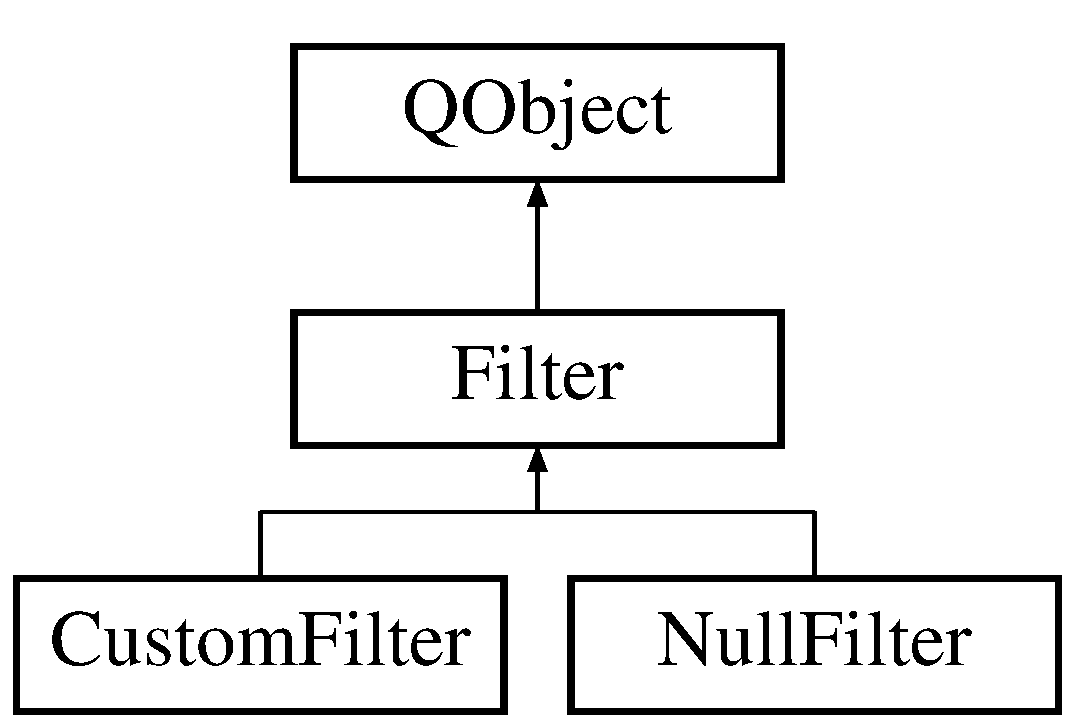
\includegraphics[height=3.000000cm]{class_filter}
\end{center}
\end{figure}
\subsection*{Public Member Functions}
\begin{DoxyCompactItemize}
\item 
\hyperlink{class_filter_a63401236b02925be21f62de930864aa7}{Filter} (Q\+Object $\ast$parent=0)
\item 
virtual Q\+Byte\+Array \hyperlink{class_filter_aa401218a142d916f84aafece09eac301}{do\+Filter} (Q\+Audio\+Format format, Q\+Byte\+Array array)=0
\item 
Q\+String \hyperlink{class_filter_a61e8bcd49b821b5e994216d87564b672}{get\+Name} () const
\item 
void \hyperlink{class_filter_ac6055d4347dd37c6f25c6c0290c50267}{set\+Name} (const Q\+String \&value)
\end{DoxyCompactItemize}


\subsection{Detailed Description}
The \hyperlink{class_filter}{Filter} class  abstract vision of filter. 

\subsection{Constructor \& Destructor Documentation}
\hypertarget{class_filter_a63401236b02925be21f62de930864aa7}{}\label{class_filter_a63401236b02925be21f62de930864aa7} 
\index{Filter@{Filter}!Filter@{Filter}}
\index{Filter@{Filter}!Filter@{Filter}}
\subsubsection{\texorpdfstring{Filter()}{Filter()}}
{\footnotesize\ttfamily Filter\+::\+Filter (\begin{DoxyParamCaption}\item[{Q\+Object $\ast$}]{parent = {\ttfamily 0} }\end{DoxyParamCaption})\hspace{0.3cm}{\ttfamily [explicit]}}



\subsection{Member Function Documentation}
\hypertarget{class_filter_aa401218a142d916f84aafece09eac301}{}\label{class_filter_aa401218a142d916f84aafece09eac301} 
\index{Filter@{Filter}!do\+Filter@{do\+Filter}}
\index{do\+Filter@{do\+Filter}!Filter@{Filter}}
\subsubsection{\texorpdfstring{do\+Filter()}{doFilter()}}
{\footnotesize\ttfamily virtual Q\+Byte\+Array Filter\+::do\+Filter (\begin{DoxyParamCaption}\item[{Q\+Audio\+Format}]{format,  }\item[{Q\+Byte\+Array}]{array }\end{DoxyParamCaption})\hspace{0.3cm}{\ttfamily [pure virtual]}}



Implemented in \hyperlink{class_custom_filter_aafa4ccbab26275b5ef223158cbb684ab}{Custom\+Filter}, and \hyperlink{class_null_filter_a738c372168e34415189cb289ead46479}{Null\+Filter}.

\hypertarget{class_filter_a61e8bcd49b821b5e994216d87564b672}{}\label{class_filter_a61e8bcd49b821b5e994216d87564b672} 
\index{Filter@{Filter}!get\+Name@{get\+Name}}
\index{get\+Name@{get\+Name}!Filter@{Filter}}
\subsubsection{\texorpdfstring{get\+Name()}{getName()}}
{\footnotesize\ttfamily Q\+String Filter\+::get\+Name (\begin{DoxyParamCaption}{ }\end{DoxyParamCaption}) const}

\hypertarget{class_filter_ac6055d4347dd37c6f25c6c0290c50267}{}\label{class_filter_ac6055d4347dd37c6f25c6c0290c50267} 
\index{Filter@{Filter}!set\+Name@{set\+Name}}
\index{set\+Name@{set\+Name}!Filter@{Filter}}
\subsubsection{\texorpdfstring{set\+Name()}{setName()}}
{\footnotesize\ttfamily void Filter\+::set\+Name (\begin{DoxyParamCaption}\item[{const Q\+String \&}]{value }\end{DoxyParamCaption})}



The documentation for this class was generated from the following files\+:\begin{DoxyCompactItemize}
\item 
app/\hyperlink{filter_8h}{filter.\+h}\item 
app/\hyperlink{filter_8cpp}{filter.\+cpp}\end{DoxyCompactItemize}

\hypertarget{class_frequency_spectrum}{}\section{Frequency\+Spectrum Class Reference}
\label{class_frequency_spectrum}\index{Frequency\+Spectrum@{Frequency\+Spectrum}}


{\ttfamily \#include $<$frequencyspectrum.\+h$>$}

\subsection*{Classes}
\begin{DoxyCompactItemize}
\item 
struct \hyperlink{struct_frequency_spectrum_1_1_element}{Element}
\end{DoxyCompactItemize}
\subsection*{Public Types}
\begin{DoxyCompactItemize}
\item 
typedef Q\+Vector$<$ \hyperlink{struct_frequency_spectrum_1_1_element}{Element} $>$\+::\hyperlink{class_frequency_spectrum_a97c7fc372f25a6caef70041f07e4e1f3}{iterator} \hyperlink{class_frequency_spectrum_a97c7fc372f25a6caef70041f07e4e1f3}{iterator}
\item 
typedef Q\+Vector$<$ \hyperlink{struct_frequency_spectrum_1_1_element}{Element} $>$\+::\hyperlink{class_frequency_spectrum_a7dee82b74b040880feb5a0de2d7ab66b}{const\+\_\+iterator} \hyperlink{class_frequency_spectrum_a7dee82b74b040880feb5a0de2d7ab66b}{const\+\_\+iterator}
\end{DoxyCompactItemize}
\subsection*{Public Member Functions}
\begin{DoxyCompactItemize}
\item 
\hyperlink{class_frequency_spectrum_a6270014538a84e1edb5cecf6c3c918ee}{Frequency\+Spectrum} (int num\+Points=0)
\item 
void \hyperlink{class_frequency_spectrum_aa7ea1c62eda905cb7674ea5c9b436aea}{reset} ()
\item 
int \hyperlink{class_frequency_spectrum_a23f805be34e28075fe7e720a71f69b7d}{count} () const
\item 
\hyperlink{struct_frequency_spectrum_1_1_element}{Element} \& \hyperlink{class_frequency_spectrum_afbe235c3468e16f7acceca10cc46537e}{operator\mbox{[}$\,$\mbox{]}} (int index)
\item 
const \hyperlink{struct_frequency_spectrum_1_1_element}{Element} \& \hyperlink{class_frequency_spectrum_a21f7b170c6a74b603acdf1587decbc42}{operator\mbox{[}$\,$\mbox{]}} (int index) const
\item 
\hyperlink{class_frequency_spectrum_a97c7fc372f25a6caef70041f07e4e1f3}{iterator} \hyperlink{class_frequency_spectrum_a92aba05b6376874d54ced70d2e81309e}{begin} ()
\item 
\hyperlink{class_frequency_spectrum_a97c7fc372f25a6caef70041f07e4e1f3}{iterator} \hyperlink{class_frequency_spectrum_aa141310e65ac810ffb006e082658dbbe}{end} ()
\item 
\hyperlink{class_frequency_spectrum_a7dee82b74b040880feb5a0de2d7ab66b}{const\+\_\+iterator} \hyperlink{class_frequency_spectrum_a0c17fa4af644afc2b9555212c80db0f5}{begin} () const
\item 
\hyperlink{class_frequency_spectrum_a7dee82b74b040880feb5a0de2d7ab66b}{const\+\_\+iterator} \hyperlink{class_frequency_spectrum_a68dac125fa1f0bca9c0cc97222db2faa}{end} () const
\end{DoxyCompactItemize}


\subsection{Detailed Description}
Represents a frequency spectrum as a series of elements, each of which consists of a frequency, an amplitude and a phase. 

\subsection{Member Typedef Documentation}
\hypertarget{class_frequency_spectrum_a7dee82b74b040880feb5a0de2d7ab66b}{}\label{class_frequency_spectrum_a7dee82b74b040880feb5a0de2d7ab66b} 
\index{Frequency\+Spectrum@{Frequency\+Spectrum}!const\+\_\+iterator@{const\+\_\+iterator}}
\index{const\+\_\+iterator@{const\+\_\+iterator}!Frequency\+Spectrum@{Frequency\+Spectrum}}
\subsubsection{\texorpdfstring{const\+\_\+iterator}{const\_iterator}}
{\footnotesize\ttfamily typedef Q\+Vector$<$\hyperlink{struct_frequency_spectrum_1_1_element}{Element}$>$\+::\hyperlink{class_frequency_spectrum_a7dee82b74b040880feb5a0de2d7ab66b}{const\+\_\+iterator} \hyperlink{class_frequency_spectrum_a7dee82b74b040880feb5a0de2d7ab66b}{Frequency\+Spectrum\+::const\+\_\+iterator}}

\hypertarget{class_frequency_spectrum_a97c7fc372f25a6caef70041f07e4e1f3}{}\label{class_frequency_spectrum_a97c7fc372f25a6caef70041f07e4e1f3} 
\index{Frequency\+Spectrum@{Frequency\+Spectrum}!iterator@{iterator}}
\index{iterator@{iterator}!Frequency\+Spectrum@{Frequency\+Spectrum}}
\subsubsection{\texorpdfstring{iterator}{iterator}}
{\footnotesize\ttfamily typedef Q\+Vector$<$\hyperlink{struct_frequency_spectrum_1_1_element}{Element}$>$\+::\hyperlink{class_frequency_spectrum_a97c7fc372f25a6caef70041f07e4e1f3}{iterator} \hyperlink{class_frequency_spectrum_a97c7fc372f25a6caef70041f07e4e1f3}{Frequency\+Spectrum\+::iterator}}



\subsection{Constructor \& Destructor Documentation}
\hypertarget{class_frequency_spectrum_a6270014538a84e1edb5cecf6c3c918ee}{}\label{class_frequency_spectrum_a6270014538a84e1edb5cecf6c3c918ee} 
\index{Frequency\+Spectrum@{Frequency\+Spectrum}!Frequency\+Spectrum@{Frequency\+Spectrum}}
\index{Frequency\+Spectrum@{Frequency\+Spectrum}!Frequency\+Spectrum@{Frequency\+Spectrum}}
\subsubsection{\texorpdfstring{Frequency\+Spectrum()}{FrequencySpectrum()}}
{\footnotesize\ttfamily Frequency\+Spectrum\+::\+Frequency\+Spectrum (\begin{DoxyParamCaption}\item[{int}]{num\+Points = {\ttfamily 0} }\end{DoxyParamCaption})}



\subsection{Member Function Documentation}
\hypertarget{class_frequency_spectrum_a92aba05b6376874d54ced70d2e81309e}{}\label{class_frequency_spectrum_a92aba05b6376874d54ced70d2e81309e} 
\index{Frequency\+Spectrum@{Frequency\+Spectrum}!begin@{begin}}
\index{begin@{begin}!Frequency\+Spectrum@{Frequency\+Spectrum}}
\subsubsection{\texorpdfstring{begin()}{begin()}\hspace{0.1cm}{\footnotesize\ttfamily [1/2]}}
{\footnotesize\ttfamily \hyperlink{class_frequency_spectrum_a97c7fc372f25a6caef70041f07e4e1f3}{Frequency\+Spectrum\+::iterator} Frequency\+Spectrum\+::begin (\begin{DoxyParamCaption}{ }\end{DoxyParamCaption})}

\hypertarget{class_frequency_spectrum_a0c17fa4af644afc2b9555212c80db0f5}{}\label{class_frequency_spectrum_a0c17fa4af644afc2b9555212c80db0f5} 
\index{Frequency\+Spectrum@{Frequency\+Spectrum}!begin@{begin}}
\index{begin@{begin}!Frequency\+Spectrum@{Frequency\+Spectrum}}
\subsubsection{\texorpdfstring{begin()}{begin()}\hspace{0.1cm}{\footnotesize\ttfamily [2/2]}}
{\footnotesize\ttfamily \hyperlink{class_frequency_spectrum_a7dee82b74b040880feb5a0de2d7ab66b}{Frequency\+Spectrum\+::const\+\_\+iterator} Frequency\+Spectrum\+::begin (\begin{DoxyParamCaption}{ }\end{DoxyParamCaption}) const}

\hypertarget{class_frequency_spectrum_a23f805be34e28075fe7e720a71f69b7d}{}\label{class_frequency_spectrum_a23f805be34e28075fe7e720a71f69b7d} 
\index{Frequency\+Spectrum@{Frequency\+Spectrum}!count@{count}}
\index{count@{count}!Frequency\+Spectrum@{Frequency\+Spectrum}}
\subsubsection{\texorpdfstring{count()}{count()}}
{\footnotesize\ttfamily int Frequency\+Spectrum\+::count (\begin{DoxyParamCaption}{ }\end{DoxyParamCaption}) const}

\hypertarget{class_frequency_spectrum_aa141310e65ac810ffb006e082658dbbe}{}\label{class_frequency_spectrum_aa141310e65ac810ffb006e082658dbbe} 
\index{Frequency\+Spectrum@{Frequency\+Spectrum}!end@{end}}
\index{end@{end}!Frequency\+Spectrum@{Frequency\+Spectrum}}
\subsubsection{\texorpdfstring{end()}{end()}\hspace{0.1cm}{\footnotesize\ttfamily [1/2]}}
{\footnotesize\ttfamily \hyperlink{class_frequency_spectrum_a97c7fc372f25a6caef70041f07e4e1f3}{Frequency\+Spectrum\+::iterator} Frequency\+Spectrum\+::end (\begin{DoxyParamCaption}{ }\end{DoxyParamCaption})}

\hypertarget{class_frequency_spectrum_a68dac125fa1f0bca9c0cc97222db2faa}{}\label{class_frequency_spectrum_a68dac125fa1f0bca9c0cc97222db2faa} 
\index{Frequency\+Spectrum@{Frequency\+Spectrum}!end@{end}}
\index{end@{end}!Frequency\+Spectrum@{Frequency\+Spectrum}}
\subsubsection{\texorpdfstring{end()}{end()}\hspace{0.1cm}{\footnotesize\ttfamily [2/2]}}
{\footnotesize\ttfamily \hyperlink{class_frequency_spectrum_a7dee82b74b040880feb5a0de2d7ab66b}{Frequency\+Spectrum\+::const\+\_\+iterator} Frequency\+Spectrum\+::end (\begin{DoxyParamCaption}{ }\end{DoxyParamCaption}) const}

\hypertarget{class_frequency_spectrum_afbe235c3468e16f7acceca10cc46537e}{}\label{class_frequency_spectrum_afbe235c3468e16f7acceca10cc46537e} 
\index{Frequency\+Spectrum@{Frequency\+Spectrum}!operator\mbox{[}\mbox{]}@{operator[]}}
\index{operator\mbox{[}\mbox{]}@{operator[]}!Frequency\+Spectrum@{Frequency\+Spectrum}}
\subsubsection{\texorpdfstring{operator[]()}{operator[]()}\hspace{0.1cm}{\footnotesize\ttfamily [1/2]}}
{\footnotesize\ttfamily \hyperlink{struct_frequency_spectrum_1_1_element}{Frequency\+Spectrum\+::\+Element} \& Frequency\+Spectrum\+::operator\mbox{[}$\,$\mbox{]} (\begin{DoxyParamCaption}\item[{int}]{index }\end{DoxyParamCaption})}

\hypertarget{class_frequency_spectrum_a21f7b170c6a74b603acdf1587decbc42}{}\label{class_frequency_spectrum_a21f7b170c6a74b603acdf1587decbc42} 
\index{Frequency\+Spectrum@{Frequency\+Spectrum}!operator\mbox{[}\mbox{]}@{operator[]}}
\index{operator\mbox{[}\mbox{]}@{operator[]}!Frequency\+Spectrum@{Frequency\+Spectrum}}
\subsubsection{\texorpdfstring{operator[]()}{operator[]()}\hspace{0.1cm}{\footnotesize\ttfamily [2/2]}}
{\footnotesize\ttfamily const \hyperlink{struct_frequency_spectrum_1_1_element}{Frequency\+Spectrum\+::\+Element} \& Frequency\+Spectrum\+::operator\mbox{[}$\,$\mbox{]} (\begin{DoxyParamCaption}\item[{int}]{index }\end{DoxyParamCaption}) const}

\hypertarget{class_frequency_spectrum_aa7ea1c62eda905cb7674ea5c9b436aea}{}\label{class_frequency_spectrum_aa7ea1c62eda905cb7674ea5c9b436aea} 
\index{Frequency\+Spectrum@{Frequency\+Spectrum}!reset@{reset}}
\index{reset@{reset}!Frequency\+Spectrum@{Frequency\+Spectrum}}
\subsubsection{\texorpdfstring{reset()}{reset()}}
{\footnotesize\ttfamily void Frequency\+Spectrum\+::reset (\begin{DoxyParamCaption}{ }\end{DoxyParamCaption})}



The documentation for this class was generated from the following files\+:\begin{DoxyCompactItemize}
\item 
app/\hyperlink{frequencyspectrum_8h}{frequencyspectrum.\+h}\item 
app/\hyperlink{frequencyspectrum_8cpp}{frequencyspectrum.\+cpp}\end{DoxyCompactItemize}

\hypertarget{class_graph}{}\section{Graph Class Reference}
\label{class_graph}\index{Graph@{Graph}}


{\ttfamily \#include $<$graph.\+h$>$}

Inheritance diagram for Graph\+:\begin{figure}[H]
\begin{center}
\leavevmode
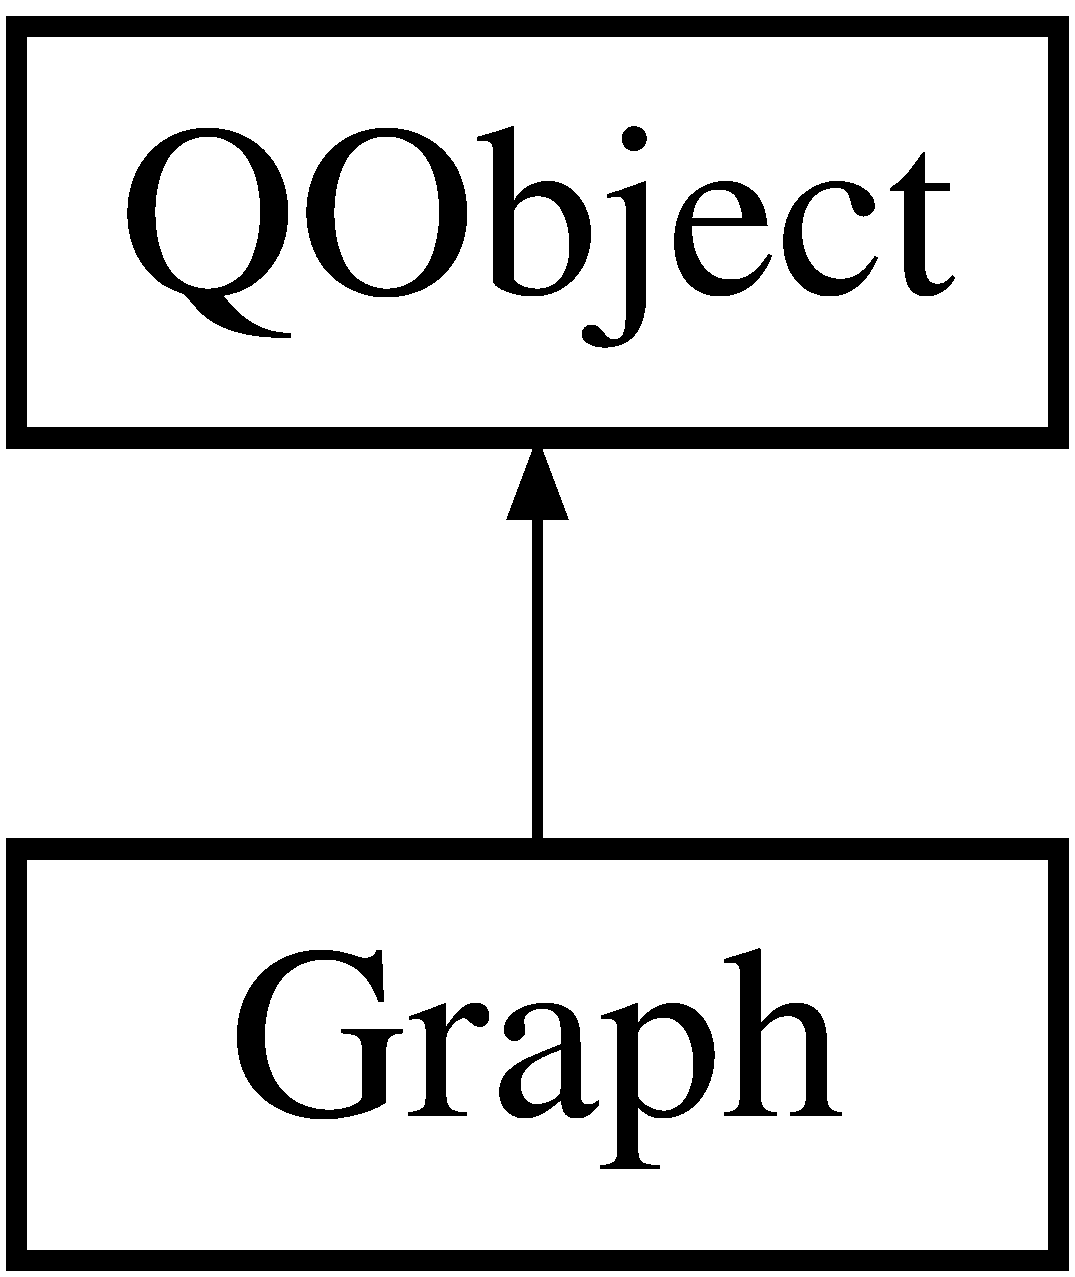
\includegraphics[height=2.000000cm]{class_graph}
\end{center}
\end{figure}
\subsection*{Public Types}
\begin{DoxyCompactItemize}
\item 
enum \hyperlink{class_graph_ab17f5821c439d7728a144639aa849501}{G\+R\+A\+P\+H\+I\+C\+T\+Y\+PE} \{ \hyperlink{class_graph_ab17f5821c439d7728a144639aa849501a7f5feb538ca9b322e492121bde60adb1}{S\+P\+E\+C\+TR} = 2, 
\hyperlink{class_graph_ab17f5821c439d7728a144639aa849501a516c601a7ca33a017e277619c22357fb}{W\+A\+VE} = 1, 
\hyperlink{class_graph_ab17f5821c439d7728a144639aa849501a91a1ac591b3ca3bf16da6c3061f02109}{S\+T\+Y\+L\+E\+\_\+\+F\+I\+L\+L\+ED}
 \}
\end{DoxyCompactItemize}
\subsection*{Public Slots}
\begin{DoxyCompactItemize}
\item 
\hyperlink{class_graph_ab17f5821c439d7728a144639aa849501}{G\+R\+A\+P\+H\+I\+C\+T\+Y\+PE} \hyperlink{class_graph_a4b6573ea1f4bb9e1803378f1f7a812de}{get\+Type} () const
\item 
void \hyperlink{class_graph_af806fda6d1e73fca3ca203c90d9e8d80}{set\+Type} (const \hyperlink{class_graph_ab17f5821c439d7728a144639aa849501}{G\+R\+A\+P\+H\+I\+C\+T\+Y\+PE} \&value)
\item 
int \hyperlink{class_graph_acd7e2b641d29b3c1e4da56903614def5}{get\+Chanel} () const
\item 
void \hyperlink{class_graph_a105d0e66343efbdcf9f59b6ca71fc88c}{set\+Chanel} (int value)
\item 
Q\+String \hyperlink{class_graph_aa58147fd7b3e9c2455147dfc2d25160e}{get\+Template\+Name} () const
\item 
void \hyperlink{class_graph_a0505bdbfb8838c729cf9ee777a082f45}{set\+Template\+Name} (const Q\+String \&value)
\item 
Q\+String \hyperlink{class_graph_afbd2fdb1dba6403125c7932d7b18fa8b}{get\+Name} () const
\item 
void \hyperlink{class_graph_ac6a95e35eefe8ab6069e45b9b05ec650}{set\+Name} (const Q\+String \&value)
\item 
int \hyperlink{class_graph_a1b9029bdcb34e7dd5e8e90eb4ae26482}{get\+Id} () const
\end{DoxyCompactItemize}
\subsection*{Public Member Functions}
\begin{DoxyCompactItemize}
\item 
\hyperlink{class_graph_a80363b329e9b6c1e2cfb34f8cc4df26e}{Q\+\_\+\+E\+N\+U\+MS} (\hyperlink{class_graph_ab17f5821c439d7728a144639aa849501}{G\+R\+A\+P\+H\+I\+C\+T\+Y\+PE}) explicit \hyperlink{class_graph}{Graph}(Q\+Object $\ast$parent=0)
\begin{DoxyCompactList}\small\item\em add enums to Q\+ML \end{DoxyCompactList}\item 
\hyperlink{class_graph_a3773c87c881cc8d499c976c025eb26c9}{Graph} (int id, Q\+String name, int chanel, \hyperlink{class_graph_ab17f5821c439d7728a144639aa849501}{G\+R\+A\+P\+H\+I\+C\+T\+Y\+PE} type, Q\+String template\+Name, Q\+Object $\ast$parent=0)
\end{DoxyCompactItemize}


\subsection{Member Enumeration Documentation}
\hypertarget{class_graph_ab17f5821c439d7728a144639aa849501}{}\label{class_graph_ab17f5821c439d7728a144639aa849501} 
\index{Graph@{Graph}!G\+R\+A\+P\+H\+I\+C\+T\+Y\+PE@{G\+R\+A\+P\+H\+I\+C\+T\+Y\+PE}}
\index{G\+R\+A\+P\+H\+I\+C\+T\+Y\+PE@{G\+R\+A\+P\+H\+I\+C\+T\+Y\+PE}!Graph@{Graph}}
\subsubsection{\texorpdfstring{G\+R\+A\+P\+H\+I\+C\+T\+Y\+PE}{GRAPHICTYPE}}
{\footnotesize\ttfamily enum \hyperlink{class_graph_ab17f5821c439d7728a144639aa849501}{Graph\+::\+G\+R\+A\+P\+H\+I\+C\+T\+Y\+PE}}

\begin{DoxyEnumFields}{Enumerator}
\raisebox{\heightof{T}}[0pt][0pt]{\index{S\+P\+E\+C\+TR@{S\+P\+E\+C\+TR}!Graph@{Graph}}\index{Graph@{Graph}!S\+P\+E\+C\+TR@{S\+P\+E\+C\+TR}}}\hypertarget{class_graph_ab17f5821c439d7728a144639aa849501a7f5feb538ca9b322e492121bde60adb1}{}\label{class_graph_ab17f5821c439d7728a144639aa849501a7f5feb538ca9b322e492121bde60adb1} 
S\+P\+E\+C\+TR&show specter \\
\hline

\raisebox{\heightof{T}}[0pt][0pt]{\index{W\+A\+VE@{W\+A\+VE}!Graph@{Graph}}\index{Graph@{Graph}!W\+A\+VE@{W\+A\+VE}}}\hypertarget{class_graph_ab17f5821c439d7728a144639aa849501a516c601a7ca33a017e277619c22357fb}{}\label{class_graph_ab17f5821c439d7728a144639aa849501a516c601a7ca33a017e277619c22357fb} 
W\+A\+VE&show form \\
\hline

\raisebox{\heightof{T}}[0pt][0pt]{\index{S\+T\+Y\+L\+E\+\_\+\+F\+I\+L\+L\+ED@{S\+T\+Y\+L\+E\+\_\+\+F\+I\+L\+L\+ED}!Graph@{Graph}}\index{Graph@{Graph}!S\+T\+Y\+L\+E\+\_\+\+F\+I\+L\+L\+ED@{S\+T\+Y\+L\+E\+\_\+\+F\+I\+L\+L\+ED}}}\hypertarget{class_graph_ab17f5821c439d7728a144639aa849501a91a1ac591b3ca3bf16da6c3061f02109}{}\label{class_graph_ab17f5821c439d7728a144639aa849501a91a1ac591b3ca3bf16da6c3061f02109} 
S\+T\+Y\+L\+E\+\_\+\+F\+I\+L\+L\+ED&\\
\hline

\end{DoxyEnumFields}


\subsection{Constructor \& Destructor Documentation}
\hypertarget{class_graph_a3773c87c881cc8d499c976c025eb26c9}{}\label{class_graph_a3773c87c881cc8d499c976c025eb26c9} 
\index{Graph@{Graph}!Graph@{Graph}}
\index{Graph@{Graph}!Graph@{Graph}}
\subsubsection{\texorpdfstring{Graph()}{Graph()}}
{\footnotesize\ttfamily Graph\+::\+Graph (\begin{DoxyParamCaption}\item[{int}]{id,  }\item[{Q\+String}]{name,  }\item[{int}]{chanel,  }\item[{\hyperlink{class_graph_ab17f5821c439d7728a144639aa849501}{Graph\+::\+G\+R\+A\+P\+H\+I\+C\+T\+Y\+PE}}]{type,  }\item[{Q\+String}]{template\+Name,  }\item[{Q\+Object $\ast$}]{parent = {\ttfamily 0} }\end{DoxyParamCaption})}



\subsection{Member Function Documentation}
\hypertarget{class_graph_acd7e2b641d29b3c1e4da56903614def5}{}\label{class_graph_acd7e2b641d29b3c1e4da56903614def5} 
\index{Graph@{Graph}!get\+Chanel@{get\+Chanel}}
\index{get\+Chanel@{get\+Chanel}!Graph@{Graph}}
\subsubsection{\texorpdfstring{get\+Chanel}{getChanel}}
{\footnotesize\ttfamily int Graph\+::get\+Chanel (\begin{DoxyParamCaption}{ }\end{DoxyParamCaption}) const\hspace{0.3cm}{\ttfamily [slot]}}

\hypertarget{class_graph_a1b9029bdcb34e7dd5e8e90eb4ae26482}{}\label{class_graph_a1b9029bdcb34e7dd5e8e90eb4ae26482} 
\index{Graph@{Graph}!get\+Id@{get\+Id}}
\index{get\+Id@{get\+Id}!Graph@{Graph}}
\subsubsection{\texorpdfstring{get\+Id}{getId}}
{\footnotesize\ttfamily int Graph\+::get\+Id (\begin{DoxyParamCaption}{ }\end{DoxyParamCaption}) const\hspace{0.3cm}{\ttfamily [slot]}}

\hypertarget{class_graph_afbd2fdb1dba6403125c7932d7b18fa8b}{}\label{class_graph_afbd2fdb1dba6403125c7932d7b18fa8b} 
\index{Graph@{Graph}!get\+Name@{get\+Name}}
\index{get\+Name@{get\+Name}!Graph@{Graph}}
\subsubsection{\texorpdfstring{get\+Name}{getName}}
{\footnotesize\ttfamily Q\+String Graph\+::get\+Name (\begin{DoxyParamCaption}{ }\end{DoxyParamCaption}) const\hspace{0.3cm}{\ttfamily [slot]}}

\hypertarget{class_graph_aa58147fd7b3e9c2455147dfc2d25160e}{}\label{class_graph_aa58147fd7b3e9c2455147dfc2d25160e} 
\index{Graph@{Graph}!get\+Template\+Name@{get\+Template\+Name}}
\index{get\+Template\+Name@{get\+Template\+Name}!Graph@{Graph}}
\subsubsection{\texorpdfstring{get\+Template\+Name}{getTemplateName}}
{\footnotesize\ttfamily Q\+String Graph\+::get\+Template\+Name (\begin{DoxyParamCaption}{ }\end{DoxyParamCaption}) const\hspace{0.3cm}{\ttfamily [slot]}}

\hypertarget{class_graph_a4b6573ea1f4bb9e1803378f1f7a812de}{}\label{class_graph_a4b6573ea1f4bb9e1803378f1f7a812de} 
\index{Graph@{Graph}!get\+Type@{get\+Type}}
\index{get\+Type@{get\+Type}!Graph@{Graph}}
\subsubsection{\texorpdfstring{get\+Type}{getType}}
{\footnotesize\ttfamily \hyperlink{class_graph_ab17f5821c439d7728a144639aa849501}{Graph\+::\+G\+R\+A\+P\+H\+I\+C\+T\+Y\+PE} Graph\+::get\+Type (\begin{DoxyParamCaption}{ }\end{DoxyParamCaption}) const\hspace{0.3cm}{\ttfamily [slot]}}

\hypertarget{class_graph_a80363b329e9b6c1e2cfb34f8cc4df26e}{}\label{class_graph_a80363b329e9b6c1e2cfb34f8cc4df26e} 
\index{Graph@{Graph}!Q\+\_\+\+E\+N\+U\+MS@{Q\+\_\+\+E\+N\+U\+MS}}
\index{Q\+\_\+\+E\+N\+U\+MS@{Q\+\_\+\+E\+N\+U\+MS}!Graph@{Graph}}
\subsubsection{\texorpdfstring{Q\+\_\+\+E\+N\+U\+M\+S()}{Q\_ENUMS()}}
{\footnotesize\ttfamily Graph\+::\+Q\+\_\+\+E\+N\+U\+MS (\begin{DoxyParamCaption}\item[{\hyperlink{class_graph_ab17f5821c439d7728a144639aa849501}{G\+R\+A\+P\+H\+I\+C\+T\+Y\+PE}}]{ }\end{DoxyParamCaption})\hspace{0.3cm}{\ttfamily [pure virtual]}}



add enums to Q\+ML 

\hypertarget{class_graph_a105d0e66343efbdcf9f59b6ca71fc88c}{}\label{class_graph_a105d0e66343efbdcf9f59b6ca71fc88c} 
\index{Graph@{Graph}!set\+Chanel@{set\+Chanel}}
\index{set\+Chanel@{set\+Chanel}!Graph@{Graph}}
\subsubsection{\texorpdfstring{set\+Chanel}{setChanel}}
{\footnotesize\ttfamily void Graph\+::set\+Chanel (\begin{DoxyParamCaption}\item[{int}]{value }\end{DoxyParamCaption})\hspace{0.3cm}{\ttfamily [slot]}}

\hypertarget{class_graph_ac6a95e35eefe8ab6069e45b9b05ec650}{}\label{class_graph_ac6a95e35eefe8ab6069e45b9b05ec650} 
\index{Graph@{Graph}!set\+Name@{set\+Name}}
\index{set\+Name@{set\+Name}!Graph@{Graph}}
\subsubsection{\texorpdfstring{set\+Name}{setName}}
{\footnotesize\ttfamily void Graph\+::set\+Name (\begin{DoxyParamCaption}\item[{const Q\+String \&}]{value }\end{DoxyParamCaption})\hspace{0.3cm}{\ttfamily [slot]}}

\hypertarget{class_graph_a0505bdbfb8838c729cf9ee777a082f45}{}\label{class_graph_a0505bdbfb8838c729cf9ee777a082f45} 
\index{Graph@{Graph}!set\+Template\+Name@{set\+Template\+Name}}
\index{set\+Template\+Name@{set\+Template\+Name}!Graph@{Graph}}
\subsubsection{\texorpdfstring{set\+Template\+Name}{setTemplateName}}
{\footnotesize\ttfamily void Graph\+::set\+Template\+Name (\begin{DoxyParamCaption}\item[{const Q\+String \&}]{value }\end{DoxyParamCaption})\hspace{0.3cm}{\ttfamily [slot]}}

\hypertarget{class_graph_af806fda6d1e73fca3ca203c90d9e8d80}{}\label{class_graph_af806fda6d1e73fca3ca203c90d9e8d80} 
\index{Graph@{Graph}!set\+Type@{set\+Type}}
\index{set\+Type@{set\+Type}!Graph@{Graph}}
\subsubsection{\texorpdfstring{set\+Type}{setType}}
{\footnotesize\ttfamily void Graph\+::set\+Type (\begin{DoxyParamCaption}\item[{const \hyperlink{class_graph_ab17f5821c439d7728a144639aa849501}{G\+R\+A\+P\+H\+I\+C\+T\+Y\+PE} \&}]{value }\end{DoxyParamCaption})\hspace{0.3cm}{\ttfamily [slot]}}



The documentation for this class was generated from the following files\+:\begin{DoxyCompactItemize}
\item 
app/\hyperlink{graph_8h}{graph.\+h}\item 
app/\hyperlink{graph_8cpp}{graph.\+cpp}\end{DoxyCompactItemize}

\hypertarget{class_graph_filter_service}{}\section{Graph\+Filter\+Service Class Reference}
\label{class_graph_filter_service}\index{Graph\+Filter\+Service@{Graph\+Filter\+Service}}


The \hyperlink{class_graph_filter_service}{Graph\+Filter\+Service} class This class acts as an intermediate element between the user interface and classes for charts.  




{\ttfamily \#include $<$graphfilterservice.\+h$>$}

Inheritance diagram for Graph\+Filter\+Service\+:\begin{figure}[H]
\begin{center}
\leavevmode
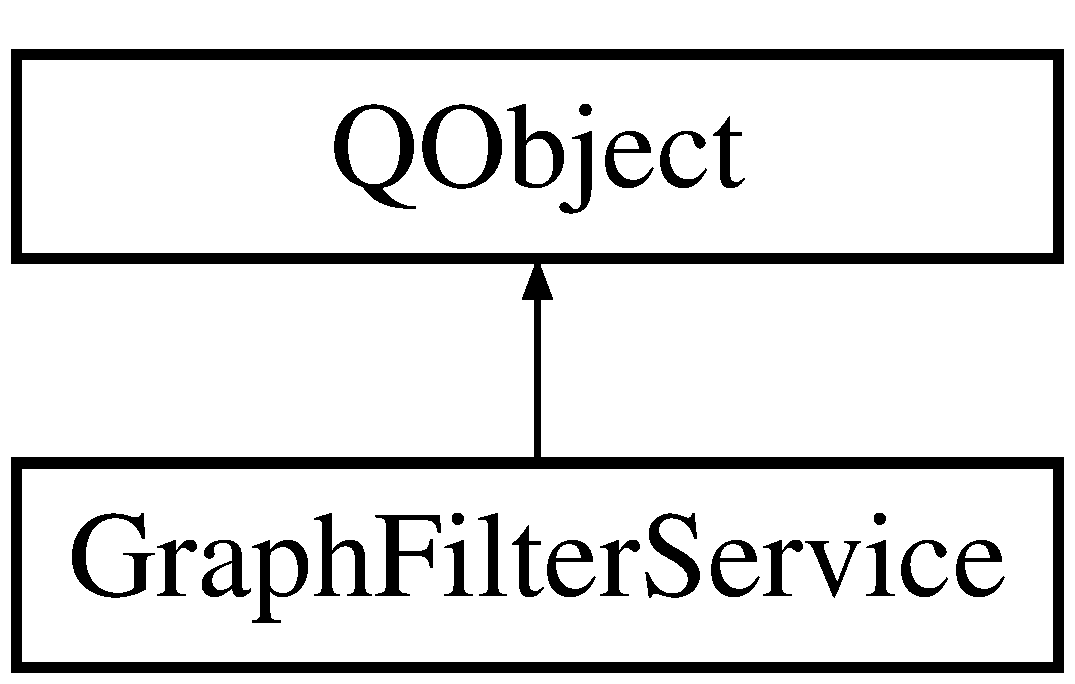
\includegraphics[height=2.000000cm]{class_graph_filter_service}
\end{center}
\end{figure}
\subsection*{Public Slots}
\begin{DoxyCompactItemize}
\item 
void \hyperlink{class_graph_filter_service_a0e7878bc2027bd8cb1480baf82783ed7}{buffer\+Changed} (qint64 position, qint64 length, const Q\+Byte\+Array \&buffer)
\item 
Q\+Byte\+Array \hyperlink{class_graph_filter_service_a399267e98d3977af552dfd0c0c39bac2}{apply\+Filters} (const Q\+Byte\+Array \&buffer)
\begin{DoxyCompactList}\small\item\em \hyperlink{class_graph_filter_service_a399267e98d3977af552dfd0c0c39bac2}{Graph\+Filter\+Service\+::apply\+Filters}. \end{DoxyCompactList}\item 
bool \hyperlink{class_graph_filter_service_a0ce26d46d68fd45bc4de9104e9b7a317}{save} (qint64 start, qint64 end, Q\+I\+O\+Device $\ast$out)
\begin{DoxyCompactList}\small\item\em save -\/ function for dump filtered data \end{DoxyCompactList}\item 
void \hyperlink{class_graph_filter_service_af02cad074674e6ff8030c2e8fc3be111}{subscribe\+Wave\+Form} (Q\+X\+Y\+Series $\ast$set, int chanel)
\begin{DoxyCompactList}\small\item\em subscribe\+Wave\+Form -\/ subscribe Q\+ML Element to visual update after update data; \end{DoxyCompactList}\item 
void \hyperlink{class_graph_filter_service_a710cfa42186e53b0ffbe9f34d57184a7}{un\+Subscribe\+Wave\+Formm} (Q\+X\+Y\+Series $\ast$set, int chanel)
\item 
void \hyperlink{class_graph_filter_service_a815f1067416248564e36f876d34c57d8}{subscribe\+Spectrum} (Q\+X\+Y\+Series $\ast$set, int chanel)
\item 
void \hyperlink{class_graph_filter_service_aae672b63fafe0403b7ae68844bbf90fa}{un\+Subscribe\+Spectrum} (Q\+X\+Y\+Series $\ast$set, int chanel)
\end{DoxyCompactItemize}
\subsection*{Public Member Functions}
\begin{DoxyCompactItemize}
\item 
\hyperlink{class_graph_filter_service_af10b79e7d0a0736df08ab20733311b67}{Graph\+Filter\+Service} (\hyperlink{class_engine}{Engine} $\ast$engine, Q\+List$<$ \hyperlink{class_filter}{Filter} $\ast$$>$ \&filters, Q\+Object $\ast$parent=0)
\begin{DoxyCompactList}\small\item\em \hyperlink{class_graph_filter_service}{Graph\+Filter\+Service}. \end{DoxyCompactList}\item 
\hyperlink{class_graph_filter_service_a9036ef6a3b6348698c9386e71371d488}{$\sim$\+Graph\+Filter\+Service} ()
\item 
Q\+String \hyperlink{class_graph_filter_service_a16e88d8a688024ab96a4e3ed6a19e238}{get\+Name} () const
\item 
void \hyperlink{class_graph_filter_service_abcbd3365d2c735616f61de87a0af8ea4}{set\+Name} (const Q\+String \&value)
\end{DoxyCompactItemize}


\subsection{Detailed Description}
The \hyperlink{class_graph_filter_service}{Graph\+Filter\+Service} class This class acts as an intermediate element between the user interface and classes for charts. 

\begin{DoxyAuthor}{Author}
Nicolas 
\end{DoxyAuthor}


\subsection{Constructor \& Destructor Documentation}
\hypertarget{class_graph_filter_service_af10b79e7d0a0736df08ab20733311b67}{}\label{class_graph_filter_service_af10b79e7d0a0736df08ab20733311b67} 
\index{Graph\+Filter\+Service@{Graph\+Filter\+Service}!Graph\+Filter\+Service@{Graph\+Filter\+Service}}
\index{Graph\+Filter\+Service@{Graph\+Filter\+Service}!Graph\+Filter\+Service@{Graph\+Filter\+Service}}
\subsubsection{\texorpdfstring{Graph\+Filter\+Service()}{GraphFilterService()}}
{\footnotesize\ttfamily Graph\+Filter\+Service\+::\+Graph\+Filter\+Service (\begin{DoxyParamCaption}\item[{\hyperlink{class_engine}{Engine} $\ast$}]{engine,  }\item[{Q\+List$<$ \hyperlink{class_filter}{Filter} $\ast$$>$ \&}]{filters,  }\item[{Q\+Object $\ast$}]{parent = {\ttfamily 0} }\end{DoxyParamCaption})}



\hyperlink{class_graph_filter_service}{Graph\+Filter\+Service}. 


\begin{DoxyParams}{Parameters}
{\em engine} & -\/ need for auto subscribe to buffer change; \\
\hline
{\em filters} & -\/ list of filters which will be apply \\
\hline
{\em parent} & \\
\hline
\end{DoxyParams}
\hypertarget{class_graph_filter_service_a9036ef6a3b6348698c9386e71371d488}{}\label{class_graph_filter_service_a9036ef6a3b6348698c9386e71371d488} 
\index{Graph\+Filter\+Service@{Graph\+Filter\+Service}!````~Graph\+Filter\+Service@{$\sim$\+Graph\+Filter\+Service}}
\index{````~Graph\+Filter\+Service@{$\sim$\+Graph\+Filter\+Service}!Graph\+Filter\+Service@{Graph\+Filter\+Service}}
\subsubsection{\texorpdfstring{$\sim$\+Graph\+Filter\+Service()}{~GraphFilterService()}}
{\footnotesize\ttfamily Graph\+Filter\+Service\+::$\sim$\+Graph\+Filter\+Service (\begin{DoxyParamCaption}{ }\end{DoxyParamCaption})}



\subsection{Member Function Documentation}
\hypertarget{class_graph_filter_service_a399267e98d3977af552dfd0c0c39bac2}{}\label{class_graph_filter_service_a399267e98d3977af552dfd0c0c39bac2} 
\index{Graph\+Filter\+Service@{Graph\+Filter\+Service}!apply\+Filters@{apply\+Filters}}
\index{apply\+Filters@{apply\+Filters}!Graph\+Filter\+Service@{Graph\+Filter\+Service}}
\subsubsection{\texorpdfstring{apply\+Filters}{applyFilters}}
{\footnotesize\ttfamily Q\+Byte\+Array Graph\+Filter\+Service\+::apply\+Filters (\begin{DoxyParamCaption}\item[{const Q\+Byte\+Array \&}]{buffer }\end{DoxyParamCaption})\hspace{0.3cm}{\ttfamily [slot]}}



\hyperlink{class_graph_filter_service_a399267e98d3977af552dfd0c0c39bac2}{Graph\+Filter\+Service\+::apply\+Filters}. 


\begin{DoxyParams}{Parameters}
{\em buffer} & -\/ data for procces \\
\hline
\end{DoxyParams}
\begin{DoxyReturn}{Returns}
performed data 
\end{DoxyReturn}
\hypertarget{class_graph_filter_service_a0e7878bc2027bd8cb1480baf82783ed7}{}\label{class_graph_filter_service_a0e7878bc2027bd8cb1480baf82783ed7} 
\index{Graph\+Filter\+Service@{Graph\+Filter\+Service}!buffer\+Changed@{buffer\+Changed}}
\index{buffer\+Changed@{buffer\+Changed}!Graph\+Filter\+Service@{Graph\+Filter\+Service}}
\subsubsection{\texorpdfstring{buffer\+Changed}{bufferChanged}}
{\footnotesize\ttfamily void Graph\+Filter\+Service\+::buffer\+Changed (\begin{DoxyParamCaption}\item[{qint64}]{position,  }\item[{qint64}]{length,  }\item[{const Q\+Byte\+Array \&}]{buffer }\end{DoxyParamCaption})\hspace{0.3cm}{\ttfamily [slot]}}

\hypertarget{class_graph_filter_service_a16e88d8a688024ab96a4e3ed6a19e238}{}\label{class_graph_filter_service_a16e88d8a688024ab96a4e3ed6a19e238} 
\index{Graph\+Filter\+Service@{Graph\+Filter\+Service}!get\+Name@{get\+Name}}
\index{get\+Name@{get\+Name}!Graph\+Filter\+Service@{Graph\+Filter\+Service}}
\subsubsection{\texorpdfstring{get\+Name()}{getName()}}
{\footnotesize\ttfamily Q\+String Graph\+Filter\+Service\+::get\+Name (\begin{DoxyParamCaption}{ }\end{DoxyParamCaption}) const}

\hypertarget{class_graph_filter_service_a0ce26d46d68fd45bc4de9104e9b7a317}{}\label{class_graph_filter_service_a0ce26d46d68fd45bc4de9104e9b7a317} 
\index{Graph\+Filter\+Service@{Graph\+Filter\+Service}!save@{save}}
\index{save@{save}!Graph\+Filter\+Service@{Graph\+Filter\+Service}}
\subsubsection{\texorpdfstring{save}{save}}
{\footnotesize\ttfamily bool Graph\+Filter\+Service\+::save (\begin{DoxyParamCaption}\item[{qint64}]{start,  }\item[{qint64}]{end,  }\item[{Q\+I\+O\+Device $\ast$}]{out }\end{DoxyParamCaption})\hspace{0.3cm}{\ttfamily [slot]}}



save -\/ function for dump filtered data 


\begin{DoxyParams}{Parameters}
{\em start} & -\/ start time in mk seconds \\
\hline
{\em end} & -\/ finish time in mk seconds \\
\hline
{\em out} & -\/ output stream (ex\+: Q\+File) \\
\hline
\end{DoxyParams}
\begin{DoxyReturn}{Returns}
is success? 
\end{DoxyReturn}
\hypertarget{class_graph_filter_service_abcbd3365d2c735616f61de87a0af8ea4}{}\label{class_graph_filter_service_abcbd3365d2c735616f61de87a0af8ea4} 
\index{Graph\+Filter\+Service@{Graph\+Filter\+Service}!set\+Name@{set\+Name}}
\index{set\+Name@{set\+Name}!Graph\+Filter\+Service@{Graph\+Filter\+Service}}
\subsubsection{\texorpdfstring{set\+Name()}{setName()}}
{\footnotesize\ttfamily void Graph\+Filter\+Service\+::set\+Name (\begin{DoxyParamCaption}\item[{const Q\+String \&}]{value }\end{DoxyParamCaption})}

\hypertarget{class_graph_filter_service_a815f1067416248564e36f876d34c57d8}{}\label{class_graph_filter_service_a815f1067416248564e36f876d34c57d8} 
\index{Graph\+Filter\+Service@{Graph\+Filter\+Service}!subscribe\+Spectrum@{subscribe\+Spectrum}}
\index{subscribe\+Spectrum@{subscribe\+Spectrum}!Graph\+Filter\+Service@{Graph\+Filter\+Service}}
\subsubsection{\texorpdfstring{subscribe\+Spectrum}{subscribeSpectrum}}
{\footnotesize\ttfamily void Graph\+Filter\+Service\+::subscribe\+Spectrum (\begin{DoxyParamCaption}\item[{Q\+X\+Y\+Series $\ast$}]{set,  }\item[{int}]{chanel }\end{DoxyParamCaption})\hspace{0.3cm}{\ttfamily [slot]}}

\hypertarget{class_graph_filter_service_af02cad074674e6ff8030c2e8fc3be111}{}\label{class_graph_filter_service_af02cad074674e6ff8030c2e8fc3be111} 
\index{Graph\+Filter\+Service@{Graph\+Filter\+Service}!subscribe\+Wave\+Form@{subscribe\+Wave\+Form}}
\index{subscribe\+Wave\+Form@{subscribe\+Wave\+Form}!Graph\+Filter\+Service@{Graph\+Filter\+Service}}
\subsubsection{\texorpdfstring{subscribe\+Wave\+Form}{subscribeWaveForm}}
{\footnotesize\ttfamily void Graph\+Filter\+Service\+::subscribe\+Wave\+Form (\begin{DoxyParamCaption}\item[{Q\+X\+Y\+Series $\ast$}]{set,  }\item[{int}]{chanel }\end{DoxyParamCaption})\hspace{0.3cm}{\ttfamily [slot]}}



subscribe\+Wave\+Form -\/ subscribe Q\+ML Element to visual update after update data; 


\begin{DoxyParams}{Parameters}
{\em set} & -\/ Q\+ML points for inject data \\
\hline
{\em chanel} & -\/ number of chanel \\
\hline
\end{DoxyParams}
\hypertarget{class_graph_filter_service_aae672b63fafe0403b7ae68844bbf90fa}{}\label{class_graph_filter_service_aae672b63fafe0403b7ae68844bbf90fa} 
\index{Graph\+Filter\+Service@{Graph\+Filter\+Service}!un\+Subscribe\+Spectrum@{un\+Subscribe\+Spectrum}}
\index{un\+Subscribe\+Spectrum@{un\+Subscribe\+Spectrum}!Graph\+Filter\+Service@{Graph\+Filter\+Service}}
\subsubsection{\texorpdfstring{un\+Subscribe\+Spectrum}{unSubscribeSpectrum}}
{\footnotesize\ttfamily void Graph\+Filter\+Service\+::un\+Subscribe\+Spectrum (\begin{DoxyParamCaption}\item[{Q\+X\+Y\+Series $\ast$}]{set,  }\item[{int}]{chanel }\end{DoxyParamCaption})\hspace{0.3cm}{\ttfamily [slot]}}

\hypertarget{class_graph_filter_service_a710cfa42186e53b0ffbe9f34d57184a7}{}\label{class_graph_filter_service_a710cfa42186e53b0ffbe9f34d57184a7} 
\index{Graph\+Filter\+Service@{Graph\+Filter\+Service}!un\+Subscribe\+Wave\+Formm@{un\+Subscribe\+Wave\+Formm}}
\index{un\+Subscribe\+Wave\+Formm@{un\+Subscribe\+Wave\+Formm}!Graph\+Filter\+Service@{Graph\+Filter\+Service}}
\subsubsection{\texorpdfstring{un\+Subscribe\+Wave\+Formm}{unSubscribeWaveFormm}}
{\footnotesize\ttfamily void Graph\+Filter\+Service\+::un\+Subscribe\+Wave\+Formm (\begin{DoxyParamCaption}\item[{Q\+X\+Y\+Series $\ast$}]{set,  }\item[{int}]{chanel }\end{DoxyParamCaption})\hspace{0.3cm}{\ttfamily [slot]}}



The documentation for this class was generated from the following files\+:\begin{DoxyCompactItemize}
\item 
app/\hyperlink{graphfilterservice_8h}{graphfilterservice.\+h}\item 
app/\hyperlink{graphfilterservice_8cpp}{graphfilterservice.\+cpp}\end{DoxyCompactItemize}

\hypertarget{class_level_meter}{}\section{Level\+Meter Class Reference}
\label{class_level_meter}\index{Level\+Meter@{Level\+Meter}}


{\ttfamily \#include $<$levelmeter.\+h$>$}

Inheritance diagram for Level\+Meter\+:\begin{figure}[H]
\begin{center}
\leavevmode
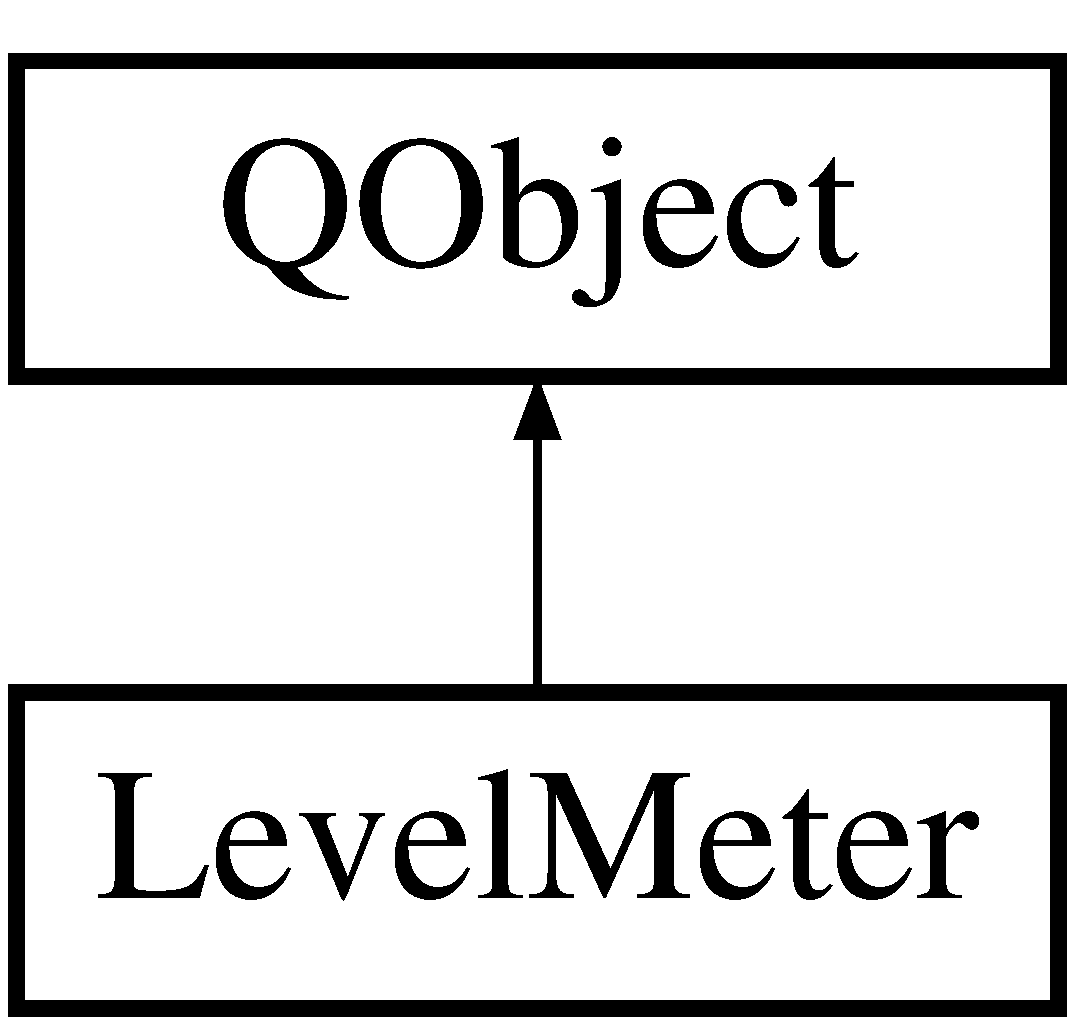
\includegraphics[height=2.000000cm]{class_level_meter}
\end{center}
\end{figure}
\subsection*{Public Slots}
\begin{DoxyCompactItemize}
\item 
void \hyperlink{class_level_meter_a53a108a6b5a8c73198c11d50173c3505}{reset} ()
\item 
void \hyperlink{class_level_meter_a5aabf54c24c8651ea834b4e8f404d5e4}{level\+Changed} (qreal rms\+Level, qreal peak\+Level, int num\+Samples)
\end{DoxyCompactItemize}
\subsection*{Public Member Functions}
\begin{DoxyCompactItemize}
\item 
\hyperlink{class_level_meter_addf17c9ccc12cfab6389a5170c5f9a49}{Level\+Meter} (Q\+Object $\ast$parent=0)
\item 
\hyperlink{class_level_meter_a28a42090bec996fdda8e804828b49b4c}{$\sim$\+Level\+Meter} ()
\item 
void \hyperlink{class_level_meter_a30abecefda651adad386ab6a643a7295}{paint\+Event} (Q\+Paint\+Event $\ast$event)
\end{DoxyCompactItemize}


\subsection{Detailed Description}
Widget which displays a vertical audio level meter, indicating the R\+MS and peak levels of the window of audio samples most recently analyzed by the \hyperlink{class_engine}{Engine}. 

\subsection{Constructor \& Destructor Documentation}
\hypertarget{class_level_meter_addf17c9ccc12cfab6389a5170c5f9a49}{}\label{class_level_meter_addf17c9ccc12cfab6389a5170c5f9a49} 
\index{Level\+Meter@{Level\+Meter}!Level\+Meter@{Level\+Meter}}
\index{Level\+Meter@{Level\+Meter}!Level\+Meter@{Level\+Meter}}
\subsubsection{\texorpdfstring{Level\+Meter()}{LevelMeter()}}
{\footnotesize\ttfamily Level\+Meter\+::\+Level\+Meter (\begin{DoxyParamCaption}\item[{Q\+Object $\ast$}]{parent = {\ttfamily 0} }\end{DoxyParamCaption})\hspace{0.3cm}{\ttfamily [explicit]}}

\hypertarget{class_level_meter_a28a42090bec996fdda8e804828b49b4c}{}\label{class_level_meter_a28a42090bec996fdda8e804828b49b4c} 
\index{Level\+Meter@{Level\+Meter}!````~Level\+Meter@{$\sim$\+Level\+Meter}}
\index{````~Level\+Meter@{$\sim$\+Level\+Meter}!Level\+Meter@{Level\+Meter}}
\subsubsection{\texorpdfstring{$\sim$\+Level\+Meter()}{~LevelMeter()}}
{\footnotesize\ttfamily Level\+Meter\+::$\sim$\+Level\+Meter (\begin{DoxyParamCaption}{ }\end{DoxyParamCaption})}



\subsection{Member Function Documentation}
\hypertarget{class_level_meter_a5aabf54c24c8651ea834b4e8f404d5e4}{}\label{class_level_meter_a5aabf54c24c8651ea834b4e8f404d5e4} 
\index{Level\+Meter@{Level\+Meter}!level\+Changed@{level\+Changed}}
\index{level\+Changed@{level\+Changed}!Level\+Meter@{Level\+Meter}}
\subsubsection{\texorpdfstring{level\+Changed}{levelChanged}}
{\footnotesize\ttfamily void Level\+Meter\+::level\+Changed (\begin{DoxyParamCaption}\item[{qreal}]{rms\+Level,  }\item[{qreal}]{peak\+Level,  }\item[{int}]{num\+Samples }\end{DoxyParamCaption})\hspace{0.3cm}{\ttfamily [slot]}}

\hypertarget{class_level_meter_a30abecefda651adad386ab6a643a7295}{}\label{class_level_meter_a30abecefda651adad386ab6a643a7295} 
\index{Level\+Meter@{Level\+Meter}!paint\+Event@{paint\+Event}}
\index{paint\+Event@{paint\+Event}!Level\+Meter@{Level\+Meter}}
\subsubsection{\texorpdfstring{paint\+Event()}{paintEvent()}}
{\footnotesize\ttfamily void Level\+Meter\+::paint\+Event (\begin{DoxyParamCaption}\item[{Q\+Paint\+Event $\ast$}]{event }\end{DoxyParamCaption})}

\hypertarget{class_level_meter_a53a108a6b5a8c73198c11d50173c3505}{}\label{class_level_meter_a53a108a6b5a8c73198c11d50173c3505} 
\index{Level\+Meter@{Level\+Meter}!reset@{reset}}
\index{reset@{reset}!Level\+Meter@{Level\+Meter}}
\subsubsection{\texorpdfstring{reset}{reset}}
{\footnotesize\ttfamily void Level\+Meter\+::reset (\begin{DoxyParamCaption}{ }\end{DoxyParamCaption})\hspace{0.3cm}{\ttfamily [slot]}}



The documentation for this class was generated from the following files\+:\begin{DoxyCompactItemize}
\item 
app/\hyperlink{levelmeter_8h}{levelmeter.\+h}\item 
app/\hyperlink{levelmeter_8cpp}{levelmeter.\+cpp}\end{DoxyCompactItemize}

\hypertarget{class_main_widget}{}\section{Main\+Widget Class Reference}
\label{class_main_widget}\index{Main\+Widget@{Main\+Widget}}


{\ttfamily \#include $<$mainwidget.\+h$>$}

Inheritance diagram for Main\+Widget\+:\begin{figure}[H]
\begin{center}
\leavevmode
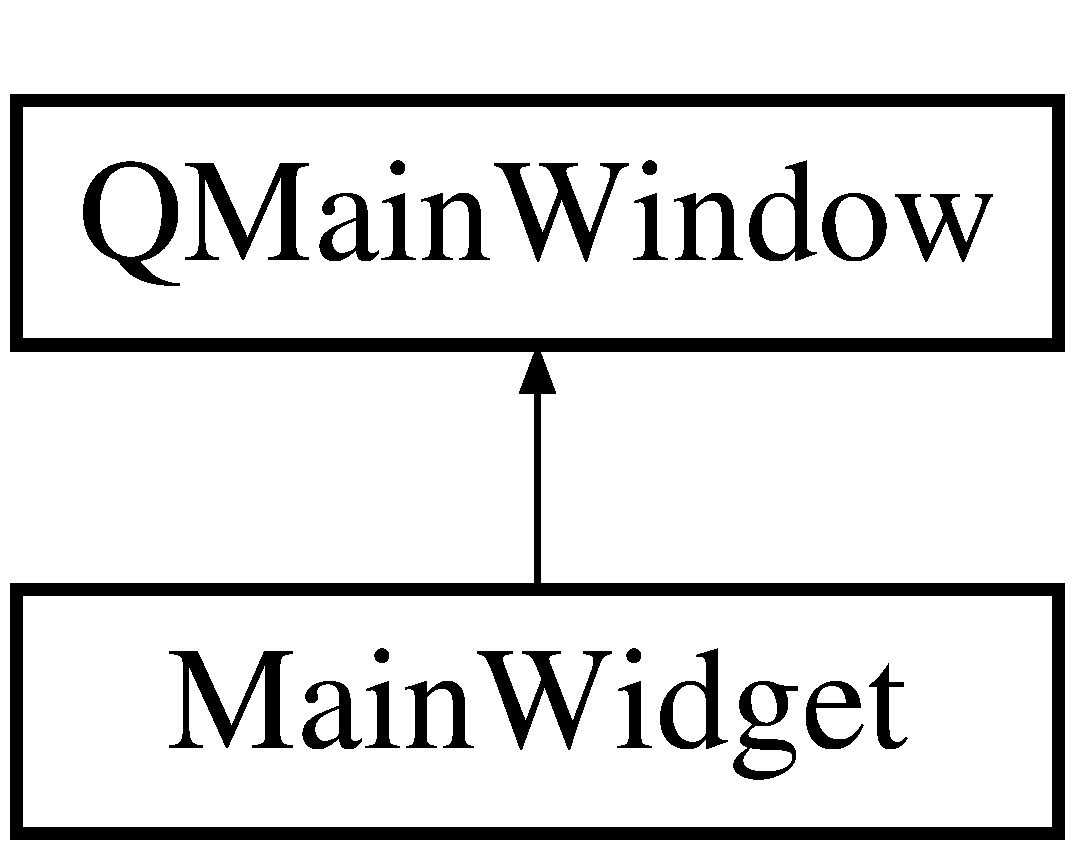
\includegraphics[height=2.000000cm]{class_main_widget}
\end{center}
\end{figure}
\subsection*{Public Slots}
\begin{DoxyCompactItemize}
\item 
void \hyperlink{class_main_widget_a8d981512811804749379b2d239e38e55}{state\+Changed} (Q\+Audio\+::\+Mode mode, Q\+Audio\+::\+State state)
\item 
void \hyperlink{class_main_widget_ab380a0a8574e1054dd6bcfd27fc903ec}{format\+Changed} (const Q\+Audio\+Format \&format)
\item 
void \hyperlink{class_main_widget_a48e11cd2d77cfd5cd495884d7d02bc56}{spectrum\+Changed} (qint64 position, qint64 length, const \hyperlink{class_frequency_spectrum}{Frequency\+Spectrum} \&spectrum)
\item 
void \hyperlink{class_main_widget_a0172df70874e3df4a32a11f6f4779310}{error\+Message} (const Q\+String \&heading, const Q\+String \&detail)
\item 
void \hyperlink{class_main_widget_ad3f4f2ec0b4354b72e6626eac21abc52}{audio\+Position\+Changed} (qint64 position)
\item 
void \hyperlink{class_main_widget_ac9c894776e1e971fe1c381b5e4b41296}{buffer\+Length\+Changed} (qint64 length)
\item 
void \hyperlink{class_main_widget_a6dd4b8c9d62111904f92ae4cbd3de0ea}{show\+File\+Dialog} ()
\item 
void \hyperlink{class_main_widget_a532dd01044abf04081c575470c89be17}{show\+Settings\+Dialog} ()
\item 
void \hyperlink{class_main_widget_a0f23ec9b7d93ae56e59e5df3e05511d6}{initialize\+Record} ()
\item 
void \hyperlink{class_main_widget_adc6c0a1a15d78df19bce3d04458c27e2}{play\+\_\+pause} ()
\item 
bool \hyperlink{class_main_widget_a4f4031960df956ff84a49af1c6494366}{is\+Full\+Screen} ()
\item 
void \hyperlink{class_main_widget_acc7c201bd760f3e416703569165b94ea}{stop} ()
\item 
double \hyperlink{class_main_widget_a13ebd72ba1fe175cf326525399e891ac}{get\+Duration} ()
\item 
double \hyperlink{class_main_widget_a12f415557fac96812d8d8d502d1f214e}{get\+Time\+Position} ()
\item 
void \hyperlink{class_main_widget_a977bb230bb404db9b34b7c3b2bf412f1}{set\+Time\+Position} (double time)
\item 
\hyperlink{class_graph}{Graph} $\ast$ \hyperlink{class_main_widget_add0a22a4b6838c7a07e48cf6a9f4ecb3}{add\+Praph} (Q\+String name, int id\+View)
\item 
Q\+List$<$ int $>$ \hyperlink{class_main_widget_ab020265c95f21766b1aa1f8c426e7f34}{get\+Praph\+Ids} (int id\+View)
\item 
\hyperlink{class_graph}{Graph} $\ast$ \hyperlink{class_main_widget_a5f07ccab510c6d5674b0a301ce0b9712}{get\+Praph\+By\+Id} (int id, int id\+View)
\item 
Q\+\_\+\+I\+N\+V\+O\+K\+A\+B\+LE Q\+String\+List \hyperlink{class_main_widget_ae77e3f796aea1d773586b1ef381061c1}{get\+Templates\+Q\+ML} ()
\item 
Q\+\_\+\+I\+N\+V\+O\+K\+A\+B\+LE bool \hyperlink{class_main_widget_adf1350b871ca05e3c3af8306d7e07acf}{subscribe\+To\+Template} (\hyperlink{class_graph}{Graph} $\ast$graph, Q\+X\+Y\+Series $\ast$set, int chanel)
\item 
Q\+\_\+\+I\+N\+V\+O\+K\+A\+B\+LE bool \hyperlink{class_main_widget_aafe021c318c70fbf579693ff767bce27}{un\+Subscribe\+To\+Template} (\hyperlink{class_graph}{Graph} $\ast$graph, Q\+X\+Y\+Series $\ast$set, int chanel)
\item 
Q\+\_\+\+I\+N\+V\+O\+K\+A\+B\+LE void \hyperlink{class_main_widget_aa52172d75102af3717d82ad3146065f1}{change\+Play\+Template} (Q\+String name)
\item 
void \hyperlink{class_main_widget_a798a61a3c09fbb3763f93c8aa7ea8a77}{switch\+Full\+Screen} ()
\begin{DoxyCompactList}\small\item\em switch to full screen mode \end{DoxyCompactList}\item 
void \hyperlink{class_main_widget_ad7b4fcd48d785d3b6d71160971e205a1}{get\+Screen\+Shot} ()
\begin{DoxyCompactList}\small\item\em create image from current tab \end{DoxyCompactList}\end{DoxyCompactItemize}
\subsection*{Signals}
\begin{DoxyCompactItemize}
\item 
void \hyperlink{class_main_widget_a7ee933a7699c2d3f6e1f489f822640a4}{mode\+Changed} (int mode)
\end{DoxyCompactItemize}
\subsection*{Public Member Functions}
\begin{DoxyCompactItemize}
\item 
\hyperlink{class_main_widget_a326fee5088b7cebaa102ed5332dd59ee}{Main\+Widget} (Q\+Widget $\ast$parent=0)
\item 
\hyperlink{class_main_widget_add21c63f8e799303a21a69da3d288c2f}{$\sim$\+Main\+Widget} ()
\item 
void \hyperlink{class_main_widget_a2e776dc0a11cab27730e7b9721701a17}{timer\+Event} (Q\+Timer\+Event $\ast$event)
\end{DoxyCompactItemize}
\subsection*{Protected Member Functions}
\begin{DoxyCompactItemize}
\item 
void \hyperlink{class_main_widget_aeeec4a8f3b1948f7cb8a54832aae29df}{key\+Release\+Event} (Q\+Key\+Event $\ast$event)
\item 
void \hyperlink{class_main_widget_a28eb2faaa16c15722645d73b2c178d8f}{key\+Press\+Event} (Q\+Key\+Event $\ast$event)
\end{DoxyCompactItemize}


\subsection{Detailed Description}
Main application widget, responsible for connecting the various UI elements to the \hyperlink{class_engine}{Engine}. 

\subsection{Constructor \& Destructor Documentation}
\hypertarget{class_main_widget_a326fee5088b7cebaa102ed5332dd59ee}{}\label{class_main_widget_a326fee5088b7cebaa102ed5332dd59ee} 
\index{Main\+Widget@{Main\+Widget}!Main\+Widget@{Main\+Widget}}
\index{Main\+Widget@{Main\+Widget}!Main\+Widget@{Main\+Widget}}
\subsubsection{\texorpdfstring{Main\+Widget()}{MainWidget()}}
{\footnotesize\ttfamily Main\+Widget\+::\+Main\+Widget (\begin{DoxyParamCaption}\item[{Q\+Widget $\ast$}]{parent = {\ttfamily 0} }\end{DoxyParamCaption})\hspace{0.3cm}{\ttfamily [explicit]}}

\hypertarget{class_main_widget_add21c63f8e799303a21a69da3d288c2f}{}\label{class_main_widget_add21c63f8e799303a21a69da3d288c2f} 
\index{Main\+Widget@{Main\+Widget}!````~Main\+Widget@{$\sim$\+Main\+Widget}}
\index{````~Main\+Widget@{$\sim$\+Main\+Widget}!Main\+Widget@{Main\+Widget}}
\subsubsection{\texorpdfstring{$\sim$\+Main\+Widget()}{~MainWidget()}}
{\footnotesize\ttfamily Main\+Widget\+::$\sim$\+Main\+Widget (\begin{DoxyParamCaption}{ }\end{DoxyParamCaption})}



\subsection{Member Function Documentation}
\hypertarget{class_main_widget_add0a22a4b6838c7a07e48cf6a9f4ecb3}{}\label{class_main_widget_add0a22a4b6838c7a07e48cf6a9f4ecb3} 
\index{Main\+Widget@{Main\+Widget}!add\+Praph@{add\+Praph}}
\index{add\+Praph@{add\+Praph}!Main\+Widget@{Main\+Widget}}
\subsubsection{\texorpdfstring{add\+Praph}{addPraph}}
{\footnotesize\ttfamily \hyperlink{class_graph}{Graph} $\ast$ Main\+Widget\+::add\+Praph (\begin{DoxyParamCaption}\item[{Q\+String}]{name,  }\item[{int}]{id\+View }\end{DoxyParamCaption})\hspace{0.3cm}{\ttfamily [slot]}}

\hypertarget{class_main_widget_ad3f4f2ec0b4354b72e6626eac21abc52}{}\label{class_main_widget_ad3f4f2ec0b4354b72e6626eac21abc52} 
\index{Main\+Widget@{Main\+Widget}!audio\+Position\+Changed@{audio\+Position\+Changed}}
\index{audio\+Position\+Changed@{audio\+Position\+Changed}!Main\+Widget@{Main\+Widget}}
\subsubsection{\texorpdfstring{audio\+Position\+Changed}{audioPositionChanged}}
{\footnotesize\ttfamily void Main\+Widget\+::audio\+Position\+Changed (\begin{DoxyParamCaption}\item[{qint64}]{position }\end{DoxyParamCaption})\hspace{0.3cm}{\ttfamily [slot]}}

\hypertarget{class_main_widget_ac9c894776e1e971fe1c381b5e4b41296}{}\label{class_main_widget_ac9c894776e1e971fe1c381b5e4b41296} 
\index{Main\+Widget@{Main\+Widget}!buffer\+Length\+Changed@{buffer\+Length\+Changed}}
\index{buffer\+Length\+Changed@{buffer\+Length\+Changed}!Main\+Widget@{Main\+Widget}}
\subsubsection{\texorpdfstring{buffer\+Length\+Changed}{bufferLengthChanged}}
{\footnotesize\ttfamily void Main\+Widget\+::buffer\+Length\+Changed (\begin{DoxyParamCaption}\item[{qint64}]{length }\end{DoxyParamCaption})\hspace{0.3cm}{\ttfamily [slot]}}

\hypertarget{class_main_widget_aa52172d75102af3717d82ad3146065f1}{}\label{class_main_widget_aa52172d75102af3717d82ad3146065f1} 
\index{Main\+Widget@{Main\+Widget}!change\+Play\+Template@{change\+Play\+Template}}
\index{change\+Play\+Template@{change\+Play\+Template}!Main\+Widget@{Main\+Widget}}
\subsubsection{\texorpdfstring{change\+Play\+Template}{changePlayTemplate}}
{\footnotesize\ttfamily void Main\+Widget\+::change\+Play\+Template (\begin{DoxyParamCaption}\item[{Q\+String}]{name }\end{DoxyParamCaption})\hspace{0.3cm}{\ttfamily [slot]}}

\hypertarget{class_main_widget_a0172df70874e3df4a32a11f6f4779310}{}\label{class_main_widget_a0172df70874e3df4a32a11f6f4779310} 
\index{Main\+Widget@{Main\+Widget}!error\+Message@{error\+Message}}
\index{error\+Message@{error\+Message}!Main\+Widget@{Main\+Widget}}
\subsubsection{\texorpdfstring{error\+Message}{errorMessage}}
{\footnotesize\ttfamily void Main\+Widget\+::error\+Message (\begin{DoxyParamCaption}\item[{const Q\+String \&}]{heading,  }\item[{const Q\+String \&}]{detail }\end{DoxyParamCaption})\hspace{0.3cm}{\ttfamily [slot]}}

\hypertarget{class_main_widget_ab380a0a8574e1054dd6bcfd27fc903ec}{}\label{class_main_widget_ab380a0a8574e1054dd6bcfd27fc903ec} 
\index{Main\+Widget@{Main\+Widget}!format\+Changed@{format\+Changed}}
\index{format\+Changed@{format\+Changed}!Main\+Widget@{Main\+Widget}}
\subsubsection{\texorpdfstring{format\+Changed}{formatChanged}}
{\footnotesize\ttfamily void Main\+Widget\+::format\+Changed (\begin{DoxyParamCaption}\item[{const Q\+Audio\+Format \&}]{format }\end{DoxyParamCaption})\hspace{0.3cm}{\ttfamily [slot]}}

\hypertarget{class_main_widget_a13ebd72ba1fe175cf326525399e891ac}{}\label{class_main_widget_a13ebd72ba1fe175cf326525399e891ac} 
\index{Main\+Widget@{Main\+Widget}!get\+Duration@{get\+Duration}}
\index{get\+Duration@{get\+Duration}!Main\+Widget@{Main\+Widget}}
\subsubsection{\texorpdfstring{get\+Duration}{getDuration}}
{\footnotesize\ttfamily double Main\+Widget\+::get\+Duration (\begin{DoxyParamCaption}{ }\end{DoxyParamCaption})\hspace{0.3cm}{\ttfamily [slot]}}

\hypertarget{class_main_widget_a5f07ccab510c6d5674b0a301ce0b9712}{}\label{class_main_widget_a5f07ccab510c6d5674b0a301ce0b9712} 
\index{Main\+Widget@{Main\+Widget}!get\+Praph\+By\+Id@{get\+Praph\+By\+Id}}
\index{get\+Praph\+By\+Id@{get\+Praph\+By\+Id}!Main\+Widget@{Main\+Widget}}
\subsubsection{\texorpdfstring{get\+Praph\+By\+Id}{getPraphById}}
{\footnotesize\ttfamily \hyperlink{class_graph}{Graph} $\ast$ Main\+Widget\+::get\+Praph\+By\+Id (\begin{DoxyParamCaption}\item[{int}]{id,  }\item[{int}]{id\+View }\end{DoxyParamCaption})\hspace{0.3cm}{\ttfamily [slot]}}

\hypertarget{class_main_widget_ab020265c95f21766b1aa1f8c426e7f34}{}\label{class_main_widget_ab020265c95f21766b1aa1f8c426e7f34} 
\index{Main\+Widget@{Main\+Widget}!get\+Praph\+Ids@{get\+Praph\+Ids}}
\index{get\+Praph\+Ids@{get\+Praph\+Ids}!Main\+Widget@{Main\+Widget}}
\subsubsection{\texorpdfstring{get\+Praph\+Ids}{getPraphIds}}
{\footnotesize\ttfamily Q\+List$<$ int $>$ Main\+Widget\+::get\+Praph\+Ids (\begin{DoxyParamCaption}\item[{int}]{id\+View }\end{DoxyParamCaption})\hspace{0.3cm}{\ttfamily [slot]}}

\hypertarget{class_main_widget_ad7b4fcd48d785d3b6d71160971e205a1}{}\label{class_main_widget_ad7b4fcd48d785d3b6d71160971e205a1} 
\index{Main\+Widget@{Main\+Widget}!get\+Screen\+Shot@{get\+Screen\+Shot}}
\index{get\+Screen\+Shot@{get\+Screen\+Shot}!Main\+Widget@{Main\+Widget}}
\subsubsection{\texorpdfstring{get\+Screen\+Shot}{getScreenShot}}
{\footnotesize\ttfamily void Main\+Widget\+::get\+Screen\+Shot (\begin{DoxyParamCaption}{ }\end{DoxyParamCaption})\hspace{0.3cm}{\ttfamily [slot]}}



create image from current tab 

\hypertarget{class_main_widget_ae77e3f796aea1d773586b1ef381061c1}{}\label{class_main_widget_ae77e3f796aea1d773586b1ef381061c1} 
\index{Main\+Widget@{Main\+Widget}!get\+Templates\+Q\+ML@{get\+Templates\+Q\+ML}}
\index{get\+Templates\+Q\+ML@{get\+Templates\+Q\+ML}!Main\+Widget@{Main\+Widget}}
\subsubsection{\texorpdfstring{get\+Templates\+Q\+ML}{getTemplatesQML}}
{\footnotesize\ttfamily Q\+String\+List Main\+Widget\+::get\+Templates\+Q\+ML (\begin{DoxyParamCaption}{ }\end{DoxyParamCaption})\hspace{0.3cm}{\ttfamily [slot]}}

\hypertarget{class_main_widget_a12f415557fac96812d8d8d502d1f214e}{}\label{class_main_widget_a12f415557fac96812d8d8d502d1f214e} 
\index{Main\+Widget@{Main\+Widget}!get\+Time\+Position@{get\+Time\+Position}}
\index{get\+Time\+Position@{get\+Time\+Position}!Main\+Widget@{Main\+Widget}}
\subsubsection{\texorpdfstring{get\+Time\+Position}{getTimePosition}}
{\footnotesize\ttfamily double Main\+Widget\+::get\+Time\+Position (\begin{DoxyParamCaption}{ }\end{DoxyParamCaption})\hspace{0.3cm}{\ttfamily [slot]}}

\hypertarget{class_main_widget_a0f23ec9b7d93ae56e59e5df3e05511d6}{}\label{class_main_widget_a0f23ec9b7d93ae56e59e5df3e05511d6} 
\index{Main\+Widget@{Main\+Widget}!initialize\+Record@{initialize\+Record}}
\index{initialize\+Record@{initialize\+Record}!Main\+Widget@{Main\+Widget}}
\subsubsection{\texorpdfstring{initialize\+Record}{initializeRecord}}
{\footnotesize\ttfamily void Main\+Widget\+::initialize\+Record (\begin{DoxyParamCaption}{ }\end{DoxyParamCaption})\hspace{0.3cm}{\ttfamily [slot]}}

\hypertarget{class_main_widget_a4f4031960df956ff84a49af1c6494366}{}\label{class_main_widget_a4f4031960df956ff84a49af1c6494366} 
\index{Main\+Widget@{Main\+Widget}!is\+Full\+Screen@{is\+Full\+Screen}}
\index{is\+Full\+Screen@{is\+Full\+Screen}!Main\+Widget@{Main\+Widget}}
\subsubsection{\texorpdfstring{is\+Full\+Screen}{isFullScreen}}
{\footnotesize\ttfamily bool Main\+Widget\+::is\+Full\+Screen (\begin{DoxyParamCaption}{ }\end{DoxyParamCaption})\hspace{0.3cm}{\ttfamily [slot]}}

\hypertarget{class_main_widget_a28eb2faaa16c15722645d73b2c178d8f}{}\label{class_main_widget_a28eb2faaa16c15722645d73b2c178d8f} 
\index{Main\+Widget@{Main\+Widget}!key\+Press\+Event@{key\+Press\+Event}}
\index{key\+Press\+Event@{key\+Press\+Event}!Main\+Widget@{Main\+Widget}}
\subsubsection{\texorpdfstring{key\+Press\+Event()}{keyPressEvent()}}
{\footnotesize\ttfamily void Main\+Widget\+::key\+Press\+Event (\begin{DoxyParamCaption}\item[{Q\+Key\+Event $\ast$}]{event }\end{DoxyParamCaption})\hspace{0.3cm}{\ttfamily [protected]}}

\hypertarget{class_main_widget_aeeec4a8f3b1948f7cb8a54832aae29df}{}\label{class_main_widget_aeeec4a8f3b1948f7cb8a54832aae29df} 
\index{Main\+Widget@{Main\+Widget}!key\+Release\+Event@{key\+Release\+Event}}
\index{key\+Release\+Event@{key\+Release\+Event}!Main\+Widget@{Main\+Widget}}
\subsubsection{\texorpdfstring{key\+Release\+Event()}{keyReleaseEvent()}}
{\footnotesize\ttfamily void Main\+Widget\+::key\+Release\+Event (\begin{DoxyParamCaption}\item[{Q\+Key\+Event $\ast$}]{event }\end{DoxyParamCaption})\hspace{0.3cm}{\ttfamily [protected]}}

\hypertarget{class_main_widget_a7ee933a7699c2d3f6e1f489f822640a4}{}\label{class_main_widget_a7ee933a7699c2d3f6e1f489f822640a4} 
\index{Main\+Widget@{Main\+Widget}!mode\+Changed@{mode\+Changed}}
\index{mode\+Changed@{mode\+Changed}!Main\+Widget@{Main\+Widget}}
\subsubsection{\texorpdfstring{mode\+Changed}{modeChanged}}
{\footnotesize\ttfamily void Main\+Widget\+::mode\+Changed (\begin{DoxyParamCaption}\item[{int}]{mode }\end{DoxyParamCaption})\hspace{0.3cm}{\ttfamily [signal]}}

\hypertarget{class_main_widget_adc6c0a1a15d78df19bce3d04458c27e2}{}\label{class_main_widget_adc6c0a1a15d78df19bce3d04458c27e2} 
\index{Main\+Widget@{Main\+Widget}!play\+\_\+pause@{play\+\_\+pause}}
\index{play\+\_\+pause@{play\+\_\+pause}!Main\+Widget@{Main\+Widget}}
\subsubsection{\texorpdfstring{play\+\_\+pause}{play\_pause}}
{\footnotesize\ttfamily void Main\+Widget\+::play\+\_\+pause (\begin{DoxyParamCaption}{ }\end{DoxyParamCaption})\hspace{0.3cm}{\ttfamily [slot]}}

\hypertarget{class_main_widget_a977bb230bb404db9b34b7c3b2bf412f1}{}\label{class_main_widget_a977bb230bb404db9b34b7c3b2bf412f1} 
\index{Main\+Widget@{Main\+Widget}!set\+Time\+Position@{set\+Time\+Position}}
\index{set\+Time\+Position@{set\+Time\+Position}!Main\+Widget@{Main\+Widget}}
\subsubsection{\texorpdfstring{set\+Time\+Position}{setTimePosition}}
{\footnotesize\ttfamily void Main\+Widget\+::set\+Time\+Position (\begin{DoxyParamCaption}\item[{double}]{time }\end{DoxyParamCaption})\hspace{0.3cm}{\ttfamily [slot]}}

\hypertarget{class_main_widget_a6dd4b8c9d62111904f92ae4cbd3de0ea}{}\label{class_main_widget_a6dd4b8c9d62111904f92ae4cbd3de0ea} 
\index{Main\+Widget@{Main\+Widget}!show\+File\+Dialog@{show\+File\+Dialog}}
\index{show\+File\+Dialog@{show\+File\+Dialog}!Main\+Widget@{Main\+Widget}}
\subsubsection{\texorpdfstring{show\+File\+Dialog}{showFileDialog}}
{\footnotesize\ttfamily void Main\+Widget\+::show\+File\+Dialog (\begin{DoxyParamCaption}{ }\end{DoxyParamCaption})\hspace{0.3cm}{\ttfamily [slot]}}

\hypertarget{class_main_widget_a532dd01044abf04081c575470c89be17}{}\label{class_main_widget_a532dd01044abf04081c575470c89be17} 
\index{Main\+Widget@{Main\+Widget}!show\+Settings\+Dialog@{show\+Settings\+Dialog}}
\index{show\+Settings\+Dialog@{show\+Settings\+Dialog}!Main\+Widget@{Main\+Widget}}
\subsubsection{\texorpdfstring{show\+Settings\+Dialog}{showSettingsDialog}}
{\footnotesize\ttfamily void Main\+Widget\+::show\+Settings\+Dialog (\begin{DoxyParamCaption}{ }\end{DoxyParamCaption})\hspace{0.3cm}{\ttfamily [slot]}}

\hypertarget{class_main_widget_a48e11cd2d77cfd5cd495884d7d02bc56}{}\label{class_main_widget_a48e11cd2d77cfd5cd495884d7d02bc56} 
\index{Main\+Widget@{Main\+Widget}!spectrum\+Changed@{spectrum\+Changed}}
\index{spectrum\+Changed@{spectrum\+Changed}!Main\+Widget@{Main\+Widget}}
\subsubsection{\texorpdfstring{spectrum\+Changed}{spectrumChanged}}
{\footnotesize\ttfamily void Main\+Widget\+::spectrum\+Changed (\begin{DoxyParamCaption}\item[{qint64}]{position,  }\item[{qint64}]{length,  }\item[{const \hyperlink{class_frequency_spectrum}{Frequency\+Spectrum} \&}]{spectrum }\end{DoxyParamCaption})\hspace{0.3cm}{\ttfamily [slot]}}

\hypertarget{class_main_widget_a8d981512811804749379b2d239e38e55}{}\label{class_main_widget_a8d981512811804749379b2d239e38e55} 
\index{Main\+Widget@{Main\+Widget}!state\+Changed@{state\+Changed}}
\index{state\+Changed@{state\+Changed}!Main\+Widget@{Main\+Widget}}
\subsubsection{\texorpdfstring{state\+Changed}{stateChanged}}
{\footnotesize\ttfamily void Main\+Widget\+::state\+Changed (\begin{DoxyParamCaption}\item[{Q\+Audio\+::\+Mode}]{mode,  }\item[{Q\+Audio\+::\+State}]{state }\end{DoxyParamCaption})\hspace{0.3cm}{\ttfamily [slot]}}

\hypertarget{class_main_widget_acc7c201bd760f3e416703569165b94ea}{}\label{class_main_widget_acc7c201bd760f3e416703569165b94ea} 
\index{Main\+Widget@{Main\+Widget}!stop@{stop}}
\index{stop@{stop}!Main\+Widget@{Main\+Widget}}
\subsubsection{\texorpdfstring{stop}{stop}}
{\footnotesize\ttfamily void Main\+Widget\+::stop (\begin{DoxyParamCaption}{ }\end{DoxyParamCaption})\hspace{0.3cm}{\ttfamily [slot]}}

\hypertarget{class_main_widget_adf1350b871ca05e3c3af8306d7e07acf}{}\label{class_main_widget_adf1350b871ca05e3c3af8306d7e07acf} 
\index{Main\+Widget@{Main\+Widget}!subscribe\+To\+Template@{subscribe\+To\+Template}}
\index{subscribe\+To\+Template@{subscribe\+To\+Template}!Main\+Widget@{Main\+Widget}}
\subsubsection{\texorpdfstring{subscribe\+To\+Template}{subscribeToTemplate}}
{\footnotesize\ttfamily bool Main\+Widget\+::subscribe\+To\+Template (\begin{DoxyParamCaption}\item[{\hyperlink{class_graph}{Graph} $\ast$}]{graph,  }\item[{Q\+X\+Y\+Series $\ast$}]{set,  }\item[{int}]{chanel }\end{DoxyParamCaption})\hspace{0.3cm}{\ttfamily [slot]}}

\hypertarget{class_main_widget_a798a61a3c09fbb3763f93c8aa7ea8a77}{}\label{class_main_widget_a798a61a3c09fbb3763f93c8aa7ea8a77} 
\index{Main\+Widget@{Main\+Widget}!switch\+Full\+Screen@{switch\+Full\+Screen}}
\index{switch\+Full\+Screen@{switch\+Full\+Screen}!Main\+Widget@{Main\+Widget}}
\subsubsection{\texorpdfstring{switch\+Full\+Screen}{switchFullScreen}}
{\footnotesize\ttfamily void Main\+Widget\+::switch\+Full\+Screen (\begin{DoxyParamCaption}{ }\end{DoxyParamCaption})\hspace{0.3cm}{\ttfamily [slot]}}



switch to full screen mode 

\hypertarget{class_main_widget_a2e776dc0a11cab27730e7b9721701a17}{}\label{class_main_widget_a2e776dc0a11cab27730e7b9721701a17} 
\index{Main\+Widget@{Main\+Widget}!timer\+Event@{timer\+Event}}
\index{timer\+Event@{timer\+Event}!Main\+Widget@{Main\+Widget}}
\subsubsection{\texorpdfstring{timer\+Event()}{timerEvent()}}
{\footnotesize\ttfamily void Main\+Widget\+::timer\+Event (\begin{DoxyParamCaption}\item[{Q\+Timer\+Event $\ast$}]{event }\end{DoxyParamCaption})}

\hypertarget{class_main_widget_aafe021c318c70fbf579693ff767bce27}{}\label{class_main_widget_aafe021c318c70fbf579693ff767bce27} 
\index{Main\+Widget@{Main\+Widget}!un\+Subscribe\+To\+Template@{un\+Subscribe\+To\+Template}}
\index{un\+Subscribe\+To\+Template@{un\+Subscribe\+To\+Template}!Main\+Widget@{Main\+Widget}}
\subsubsection{\texorpdfstring{un\+Subscribe\+To\+Template}{unSubscribeToTemplate}}
{\footnotesize\ttfamily bool Main\+Widget\+::un\+Subscribe\+To\+Template (\begin{DoxyParamCaption}\item[{\hyperlink{class_graph}{Graph} $\ast$}]{graph,  }\item[{Q\+X\+Y\+Series $\ast$}]{set,  }\item[{int}]{chanel }\end{DoxyParamCaption})\hspace{0.3cm}{\ttfamily [slot]}}



The documentation for this class was generated from the following files\+:\begin{DoxyCompactItemize}
\item 
app/\hyperlink{mainwidget_8h}{mainwidget.\+h}\item 
app/\hyperlink{mainwidget_8cpp}{mainwidget.\+cpp}\end{DoxyCompactItemize}

\hypertarget{class_null_debug}{}\section{Null\+Debug Class Reference}
\label{class_null_debug}\index{Null\+Debug@{Null\+Debug}}


{\ttfamily \#include $<$utils.\+h$>$}

\subsection*{Public Member Functions}
\begin{DoxyCompactItemize}
\item 
{\footnotesize template$<$typename T $>$ }\\\hyperlink{class_null_debug}{Null\+Debug} \& \hyperlink{class_null_debug_a51f2c613f1937fc05c9b1c74e53253f9}{operator$<$$<$} (const T \&)
\end{DoxyCompactItemize}


\subsection{Member Function Documentation}
\hypertarget{class_null_debug_a51f2c613f1937fc05c9b1c74e53253f9}{}\label{class_null_debug_a51f2c613f1937fc05c9b1c74e53253f9} 
\index{Null\+Debug@{Null\+Debug}!operator$<$$<$@{operator$<$$<$}}
\index{operator$<$$<$@{operator$<$$<$}!Null\+Debug@{Null\+Debug}}
\subsubsection{\texorpdfstring{operator$<$$<$()}{operator<<()}}
{\footnotesize\ttfamily template$<$typename T $>$ \\
\hyperlink{class_null_debug}{Null\+Debug}\& Null\+Debug\+::operator$<$$<$ (\begin{DoxyParamCaption}\item[{const T \&}]{ }\end{DoxyParamCaption})\hspace{0.3cm}{\ttfamily [inline]}}



The documentation for this class was generated from the following file\+:\begin{DoxyCompactItemize}
\item 
app/\hyperlink{utils_8h}{utils.\+h}\end{DoxyCompactItemize}

\hypertarget{class_null_filter}{}\section{Null\+Filter Class Reference}
\label{class_null_filter}\index{Null\+Filter@{Null\+Filter}}


The \hyperlink{class_null_filter}{Null\+Filter} class.  




{\ttfamily \#include $<$nullfilter.\+h$>$}

Inheritance diagram for Null\+Filter\+:\begin{figure}[H]
\begin{center}
\leavevmode
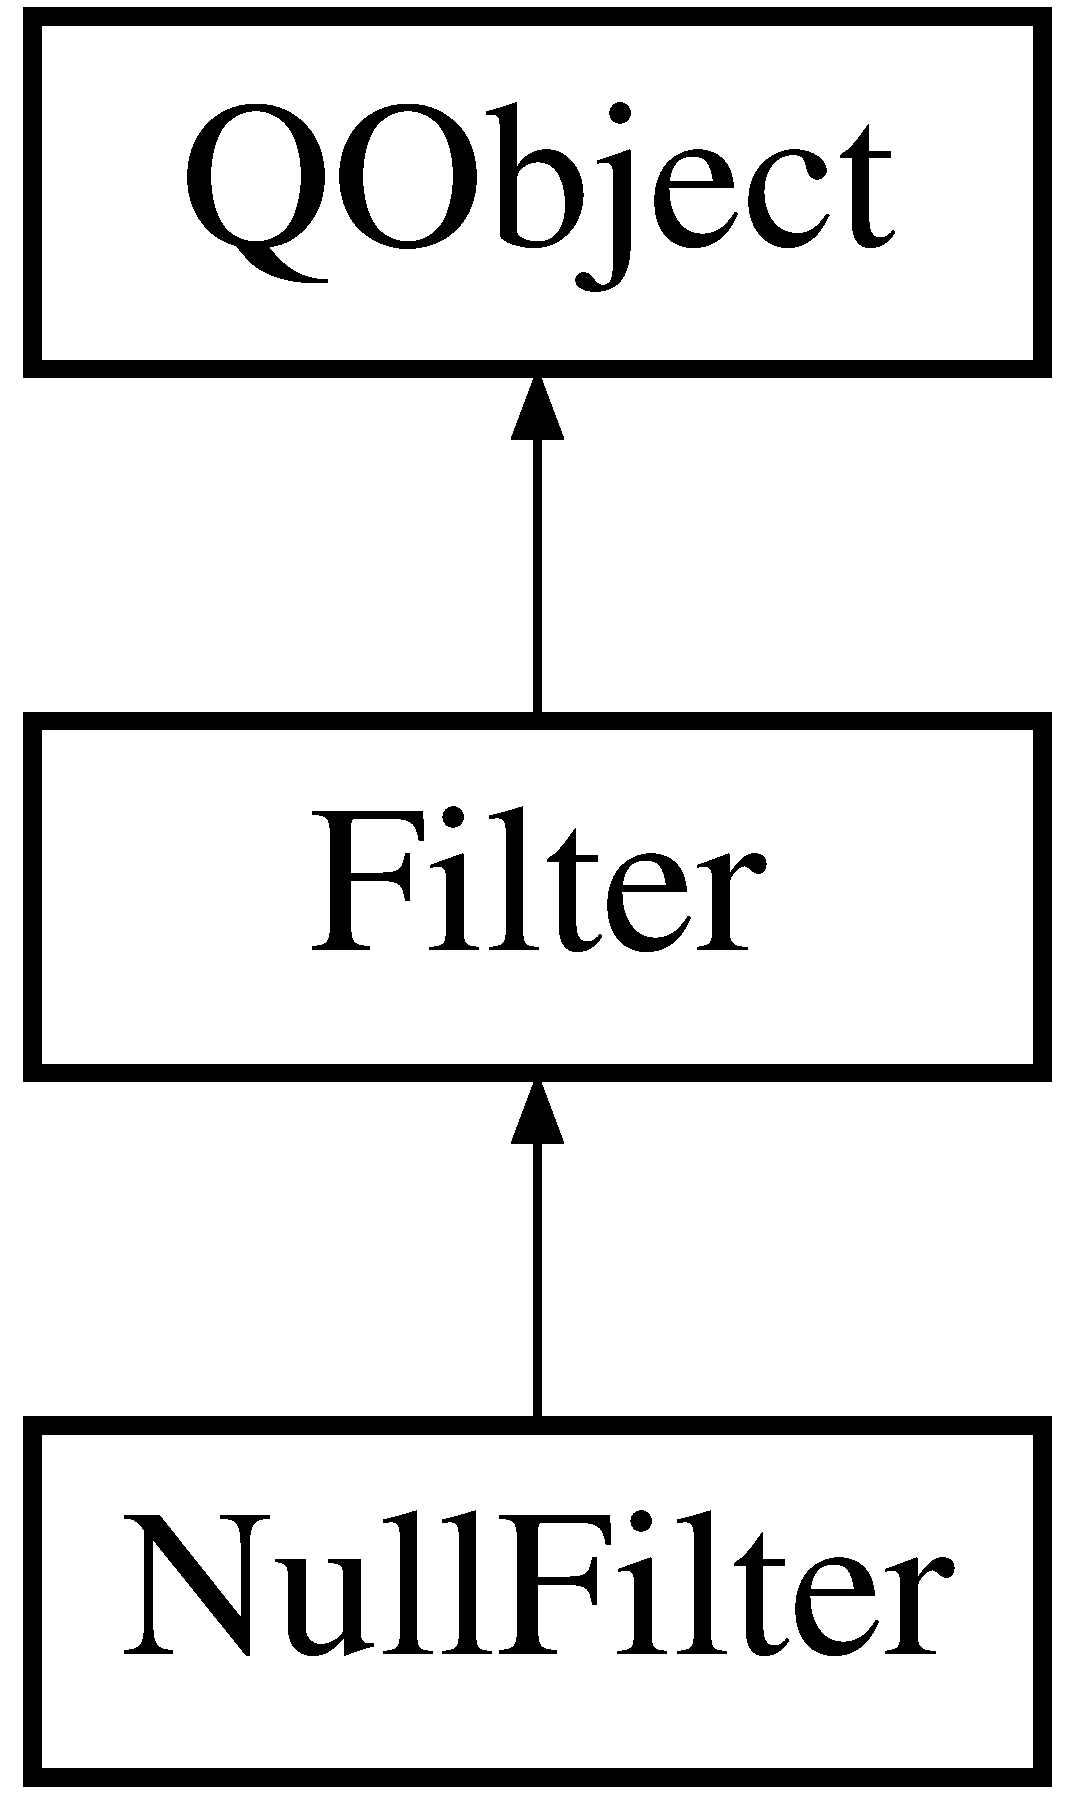
\includegraphics[height=3.000000cm]{class_null_filter}
\end{center}
\end{figure}
\subsection*{Public Member Functions}
\begin{DoxyCompactItemize}
\item 
\hyperlink{class_null_filter_aaddca4e32038999a377a4a8a37531d85}{Null\+Filter} ()
\item 
Q\+Byte\+Array \hyperlink{class_null_filter_a738c372168e34415189cb289ead46479}{do\+Filter} (Q\+Audio\+Format format, Q\+Byte\+Array array)
\end{DoxyCompactItemize}


\subsection{Detailed Description}
The \hyperlink{class_null_filter}{Null\+Filter} class. 

\begin{DoxyAuthor}{Author}
Nicolas 
\end{DoxyAuthor}


\subsection{Constructor \& Destructor Documentation}
\hypertarget{class_null_filter_aaddca4e32038999a377a4a8a37531d85}{}\label{class_null_filter_aaddca4e32038999a377a4a8a37531d85} 
\index{Null\+Filter@{Null\+Filter}!Null\+Filter@{Null\+Filter}}
\index{Null\+Filter@{Null\+Filter}!Null\+Filter@{Null\+Filter}}
\subsubsection{\texorpdfstring{Null\+Filter()}{NullFilter()}}
{\footnotesize\ttfamily Null\+Filter\+::\+Null\+Filter (\begin{DoxyParamCaption}{ }\end{DoxyParamCaption})}



\subsection{Member Function Documentation}
\hypertarget{class_null_filter_a738c372168e34415189cb289ead46479}{}\label{class_null_filter_a738c372168e34415189cb289ead46479} 
\index{Null\+Filter@{Null\+Filter}!do\+Filter@{do\+Filter}}
\index{do\+Filter@{do\+Filter}!Null\+Filter@{Null\+Filter}}
\subsubsection{\texorpdfstring{do\+Filter()}{doFilter()}}
{\footnotesize\ttfamily Q\+Byte\+Array Null\+Filter\+::do\+Filter (\begin{DoxyParamCaption}\item[{Q\+Audio\+Format}]{format,  }\item[{Q\+Byte\+Array}]{array }\end{DoxyParamCaption})\hspace{0.3cm}{\ttfamily [virtual]}}



Implements \hyperlink{class_filter_aa401218a142d916f84aafece09eac301}{Filter}.



The documentation for this class was generated from the following files\+:\begin{DoxyCompactItemize}
\item 
app/\hyperlink{nullfilter_8h}{nullfilter.\+h}\item 
app/\hyperlink{nullfilter_8cpp}{nullfilter.\+cpp}\end{DoxyCompactItemize}

\hypertarget{class_power_of_two}{}\section{Power\+Of\+Two$<$ N $>$ Class Template Reference}
\label{class_power_of_two}\index{Power\+Of\+Two$<$ N $>$@{Power\+Of\+Two$<$ N $>$}}


{\ttfamily \#include $<$utils.\+h$>$}

\subsection*{Static Public Attributes}
\begin{DoxyCompactItemize}
\item 
static const int \hyperlink{class_power_of_two_a0bdb930d07970b60ed41542fc7ec0765}{Result} = \hyperlink{class_power_of_two}{Power\+Of\+Two}$<$N-\/1$>$\+::Result $\ast$ 2
\end{DoxyCompactItemize}


\subsection{Member Data Documentation}
\hypertarget{class_power_of_two_a0bdb930d07970b60ed41542fc7ec0765}{}\label{class_power_of_two_a0bdb930d07970b60ed41542fc7ec0765} 
\index{Power\+Of\+Two@{Power\+Of\+Two}!Result@{Result}}
\index{Result@{Result}!Power\+Of\+Two@{Power\+Of\+Two}}
\subsubsection{\texorpdfstring{Result}{Result}}
{\footnotesize\ttfamily template$<$int N$>$ \\
const int \hyperlink{class_power_of_two}{Power\+Of\+Two}$<$ N $>$\+::Result = \hyperlink{class_power_of_two}{Power\+Of\+Two}$<$N-\/1$>$\+::Result $\ast$ 2\hspace{0.3cm}{\ttfamily [static]}}



The documentation for this class was generated from the following file\+:\begin{DoxyCompactItemize}
\item 
app/\hyperlink{utils_8h}{utils.\+h}\end{DoxyCompactItemize}

\hypertarget{class_power_of_two_3_010_01_4}{}\section{Power\+Of\+Two$<$ 0 $>$ Class Template Reference}
\label{class_power_of_two_3_010_01_4}\index{Power\+Of\+Two$<$ 0 $>$@{Power\+Of\+Two$<$ 0 $>$}}


{\ttfamily \#include $<$utils.\+h$>$}

\subsection*{Static Public Attributes}
\begin{DoxyCompactItemize}
\item 
static const int \hyperlink{class_power_of_two_3_010_01_4_a5f4e473a60ab5b3859b92b45835a71cd}{Result} = 1
\end{DoxyCompactItemize}


\subsection{Member Data Documentation}
\hypertarget{class_power_of_two_3_010_01_4_a5f4e473a60ab5b3859b92b45835a71cd}{}\label{class_power_of_two_3_010_01_4_a5f4e473a60ab5b3859b92b45835a71cd} 
\index{Power\+Of\+Two$<$ 0 $>$@{Power\+Of\+Two$<$ 0 $>$}!Result@{Result}}
\index{Result@{Result}!Power\+Of\+Two$<$ 0 $>$@{Power\+Of\+Two$<$ 0 $>$}}
\subsubsection{\texorpdfstring{Result}{Result}}
{\footnotesize\ttfamily const int \hyperlink{class_power_of_two}{Power\+Of\+Two}$<$ 0 $>$\+::Result = 1\hspace{0.3cm}{\ttfamily [static]}}



The documentation for this class was generated from the following file\+:\begin{DoxyCompactItemize}
\item 
app/\hyperlink{utils_8h}{utils.\+h}\end{DoxyCompactItemize}

\hypertarget{class_progress_bar}{}\section{Progress\+Bar Class Reference}
\label{class_progress_bar}\index{Progress\+Bar@{Progress\+Bar}}


{\ttfamily \#include $<$progressbar.\+h$>$}

Inheritance diagram for Progress\+Bar\+:\begin{figure}[H]
\begin{center}
\leavevmode
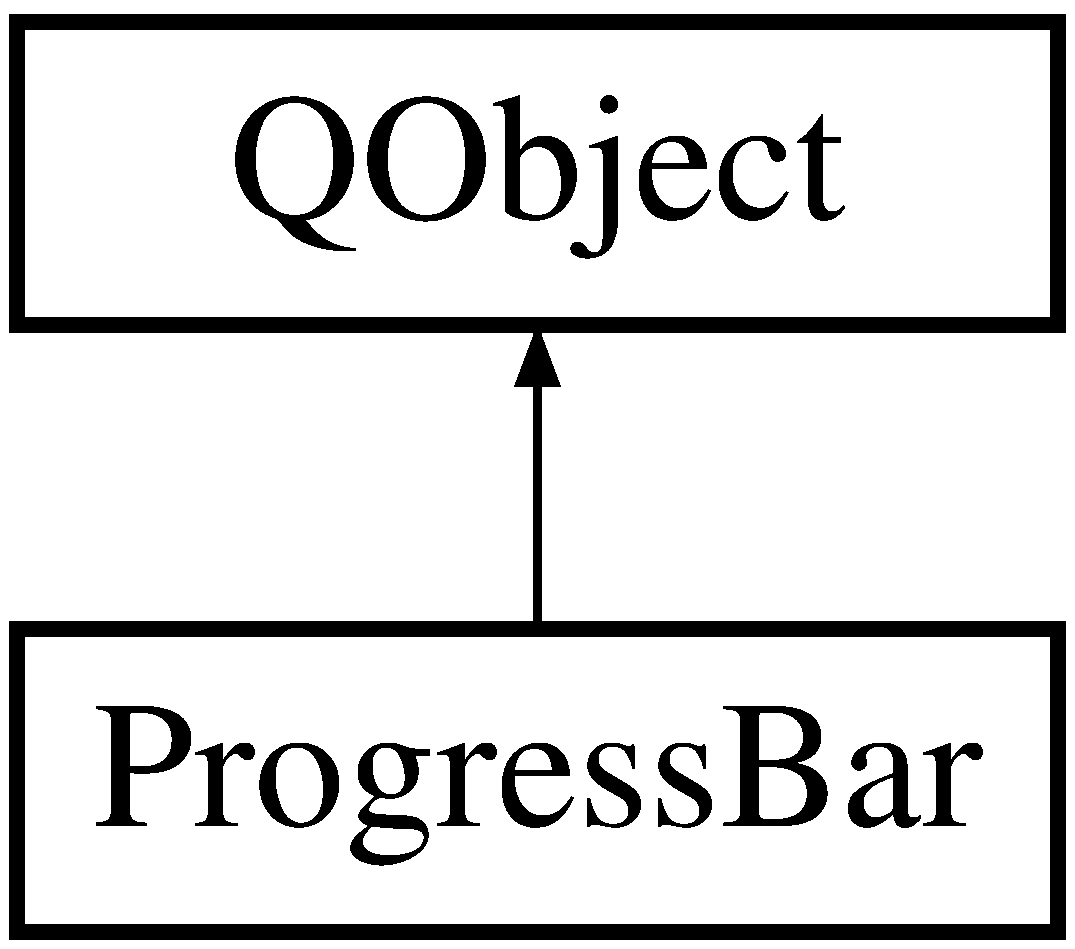
\includegraphics[height=2.000000cm]{class_progress_bar}
\end{center}
\end{figure}
\subsection*{Public Slots}
\begin{DoxyCompactItemize}
\item 
void \hyperlink{class_progress_bar_a3b191a0ae258461a6be7a8e6408c4751}{buffer\+Length\+Changed} (qint64 length)
\item 
void \hyperlink{class_progress_bar_af3575d9c0166bf9cd5dfe46b66ba1142}{record\+Position\+Changed} (qint64 record\+Position)
\item 
void \hyperlink{class_progress_bar_af664f472f1c6832796c4e0a280a7aeed}{play\+Position\+Changed} (qint64 play\+Position)
\item 
void \hyperlink{class_progress_bar_a5df10736f27e956424de9cd77dd11956}{window\+Changed} (qint64 position, qint64 length)
\end{DoxyCompactItemize}
\subsection*{Public Member Functions}
\begin{DoxyCompactItemize}
\item 
\hyperlink{class_progress_bar_a996d2532fcf95da096907a1a272052e4}{Progress\+Bar} (Q\+Object $\ast$parent=0)
\item 
\hyperlink{class_progress_bar_aa0ced60c0ade467a4602c35443e7bc78}{$\sim$\+Progress\+Bar} ()
\item 
void \hyperlink{class_progress_bar_a9ccd597a098a693f9364741fc69a3de2}{reset} ()
\end{DoxyCompactItemize}


\subsection{Detailed Description}
Widget which displays a the current fill state of the \hyperlink{class_engine}{Engine}\textquotesingle{}s internal buffer, and the current play/record position within that buffer. 

\subsection{Constructor \& Destructor Documentation}
\hypertarget{class_progress_bar_a996d2532fcf95da096907a1a272052e4}{}\label{class_progress_bar_a996d2532fcf95da096907a1a272052e4} 
\index{Progress\+Bar@{Progress\+Bar}!Progress\+Bar@{Progress\+Bar}}
\index{Progress\+Bar@{Progress\+Bar}!Progress\+Bar@{Progress\+Bar}}
\subsubsection{\texorpdfstring{Progress\+Bar()}{ProgressBar()}}
{\footnotesize\ttfamily Progress\+Bar\+::\+Progress\+Bar (\begin{DoxyParamCaption}\item[{Q\+Object $\ast$}]{parent = {\ttfamily 0} }\end{DoxyParamCaption})\hspace{0.3cm}{\ttfamily [explicit]}}

\hypertarget{class_progress_bar_aa0ced60c0ade467a4602c35443e7bc78}{}\label{class_progress_bar_aa0ced60c0ade467a4602c35443e7bc78} 
\index{Progress\+Bar@{Progress\+Bar}!````~Progress\+Bar@{$\sim$\+Progress\+Bar}}
\index{````~Progress\+Bar@{$\sim$\+Progress\+Bar}!Progress\+Bar@{Progress\+Bar}}
\subsubsection{\texorpdfstring{$\sim$\+Progress\+Bar()}{~ProgressBar()}}
{\footnotesize\ttfamily Progress\+Bar\+::$\sim$\+Progress\+Bar (\begin{DoxyParamCaption}{ }\end{DoxyParamCaption})}



\subsection{Member Function Documentation}
\hypertarget{class_progress_bar_a3b191a0ae258461a6be7a8e6408c4751}{}\label{class_progress_bar_a3b191a0ae258461a6be7a8e6408c4751} 
\index{Progress\+Bar@{Progress\+Bar}!buffer\+Length\+Changed@{buffer\+Length\+Changed}}
\index{buffer\+Length\+Changed@{buffer\+Length\+Changed}!Progress\+Bar@{Progress\+Bar}}
\subsubsection{\texorpdfstring{buffer\+Length\+Changed}{bufferLengthChanged}}
{\footnotesize\ttfamily void Progress\+Bar\+::buffer\+Length\+Changed (\begin{DoxyParamCaption}\item[{qint64}]{length }\end{DoxyParamCaption})\hspace{0.3cm}{\ttfamily [slot]}}

\hypertarget{class_progress_bar_af664f472f1c6832796c4e0a280a7aeed}{}\label{class_progress_bar_af664f472f1c6832796c4e0a280a7aeed} 
\index{Progress\+Bar@{Progress\+Bar}!play\+Position\+Changed@{play\+Position\+Changed}}
\index{play\+Position\+Changed@{play\+Position\+Changed}!Progress\+Bar@{Progress\+Bar}}
\subsubsection{\texorpdfstring{play\+Position\+Changed}{playPositionChanged}}
{\footnotesize\ttfamily void Progress\+Bar\+::play\+Position\+Changed (\begin{DoxyParamCaption}\item[{qint64}]{play\+Position }\end{DoxyParamCaption})\hspace{0.3cm}{\ttfamily [slot]}}

\hypertarget{class_progress_bar_af3575d9c0166bf9cd5dfe46b66ba1142}{}\label{class_progress_bar_af3575d9c0166bf9cd5dfe46b66ba1142} 
\index{Progress\+Bar@{Progress\+Bar}!record\+Position\+Changed@{record\+Position\+Changed}}
\index{record\+Position\+Changed@{record\+Position\+Changed}!Progress\+Bar@{Progress\+Bar}}
\subsubsection{\texorpdfstring{record\+Position\+Changed}{recordPositionChanged}}
{\footnotesize\ttfamily void Progress\+Bar\+::record\+Position\+Changed (\begin{DoxyParamCaption}\item[{qint64}]{record\+Position }\end{DoxyParamCaption})\hspace{0.3cm}{\ttfamily [slot]}}

\hypertarget{class_progress_bar_a9ccd597a098a693f9364741fc69a3de2}{}\label{class_progress_bar_a9ccd597a098a693f9364741fc69a3de2} 
\index{Progress\+Bar@{Progress\+Bar}!reset@{reset}}
\index{reset@{reset}!Progress\+Bar@{Progress\+Bar}}
\subsubsection{\texorpdfstring{reset()}{reset()}}
{\footnotesize\ttfamily void Progress\+Bar\+::reset (\begin{DoxyParamCaption}{ }\end{DoxyParamCaption})}

\hypertarget{class_progress_bar_a5df10736f27e956424de9cd77dd11956}{}\label{class_progress_bar_a5df10736f27e956424de9cd77dd11956} 
\index{Progress\+Bar@{Progress\+Bar}!window\+Changed@{window\+Changed}}
\index{window\+Changed@{window\+Changed}!Progress\+Bar@{Progress\+Bar}}
\subsubsection{\texorpdfstring{window\+Changed}{windowChanged}}
{\footnotesize\ttfamily void Progress\+Bar\+::window\+Changed (\begin{DoxyParamCaption}\item[{qint64}]{position,  }\item[{qint64}]{length }\end{DoxyParamCaption})\hspace{0.3cm}{\ttfamily [slot]}}



The documentation for this class was generated from the following files\+:\begin{DoxyCompactItemize}
\item 
app/\hyperlink{progressbar_8h}{progressbar.\+h}\item 
app/\hyperlink{progressbar_8cpp}{progressbar.\+cpp}\end{DoxyCompactItemize}

\hypertarget{struct_r_i_f_f_header}{}\section{R\+I\+F\+F\+Header Struct Reference}
\label{struct_r_i_f_f_header}\index{R\+I\+F\+F\+Header@{R\+I\+F\+F\+Header}}
\subsection*{Public Attributes}
\begin{DoxyCompactItemize}
\item 
\hyperlink{structchunk}{chunk} \hyperlink{struct_r_i_f_f_header_a3576246914fcd14ee6edeb9625e7074e}{descriptor}
\item 
char \hyperlink{struct_r_i_f_f_header_a2bc63e3bed286dd8216ee2542e729d03}{type} \mbox{[}4\mbox{]}
\end{DoxyCompactItemize}


\subsection{Member Data Documentation}
\hypertarget{struct_r_i_f_f_header_a3576246914fcd14ee6edeb9625e7074e}{}\label{struct_r_i_f_f_header_a3576246914fcd14ee6edeb9625e7074e} 
\index{R\+I\+F\+F\+Header@{R\+I\+F\+F\+Header}!descriptor@{descriptor}}
\index{descriptor@{descriptor}!R\+I\+F\+F\+Header@{R\+I\+F\+F\+Header}}
\subsubsection{\texorpdfstring{descriptor}{descriptor}}
{\footnotesize\ttfamily \hyperlink{structchunk}{chunk} R\+I\+F\+F\+Header\+::descriptor}

\hypertarget{struct_r_i_f_f_header_a2bc63e3bed286dd8216ee2542e729d03}{}\label{struct_r_i_f_f_header_a2bc63e3bed286dd8216ee2542e729d03} 
\index{R\+I\+F\+F\+Header@{R\+I\+F\+F\+Header}!type@{type}}
\index{type@{type}!R\+I\+F\+F\+Header@{R\+I\+F\+F\+Header}}
\subsubsection{\texorpdfstring{type}{type}}
{\footnotesize\ttfamily char R\+I\+F\+F\+Header\+::type\mbox{[}4\mbox{]}}



The documentation for this struct was generated from the following file\+:\begin{DoxyCompactItemize}
\item 
app/\hyperlink{wavfile_8cpp}{wavfile.\+cpp}\end{DoxyCompactItemize}

\hypertarget{struct_series_chanel}{}\section{Series\+Chanel Struct Reference}
\label{struct_series_chanel}\index{Series\+Chanel@{Series\+Chanel}}


{\ttfamily \#include $<$datasource.\+h$>$}

\subsection*{Public Member Functions}
\begin{DoxyCompactItemize}
\item 
\hyperlink{struct_series_chanel_aa9acfa3be048a0729de56b4373df478a}{Series\+Chanel} (Q\+Abstract\+Series $\ast$\hyperlink{struct_series_chanel_a3cb05afb46b3d15a4896b9a534e6a9dc}{series}, int \hyperlink{struct_series_chanel_aa8765a5a77663bd414058b73f922265f}{chanel})
\item 
bool \hyperlink{struct_series_chanel_a48df63740dd69cd7e34b4f96e1015003}{operator==} (\hyperlink{struct_series_chanel}{Series\+Chanel} other)
\end{DoxyCompactItemize}
\subsection*{Public Attributes}
\begin{DoxyCompactItemize}
\item 
Q\+Abstract\+Series $\ast$ \hyperlink{struct_series_chanel_a3cb05afb46b3d15a4896b9a534e6a9dc}{series}
\item 
int \hyperlink{struct_series_chanel_aa8765a5a77663bd414058b73f922265f}{chanel}
\end{DoxyCompactItemize}


\subsection{Constructor \& Destructor Documentation}
\hypertarget{struct_series_chanel_aa9acfa3be048a0729de56b4373df478a}{}\label{struct_series_chanel_aa9acfa3be048a0729de56b4373df478a} 
\index{Series\+Chanel@{Series\+Chanel}!Series\+Chanel@{Series\+Chanel}}
\index{Series\+Chanel@{Series\+Chanel}!Series\+Chanel@{Series\+Chanel}}
\subsubsection{\texorpdfstring{Series\+Chanel()}{SeriesChanel()}}
{\footnotesize\ttfamily Series\+Chanel\+::\+Series\+Chanel (\begin{DoxyParamCaption}\item[{Q\+Abstract\+Series $\ast$}]{series,  }\item[{int}]{chanel }\end{DoxyParamCaption})\hspace{0.3cm}{\ttfamily [inline]}}



\subsection{Member Function Documentation}
\hypertarget{struct_series_chanel_a48df63740dd69cd7e34b4f96e1015003}{}\label{struct_series_chanel_a48df63740dd69cd7e34b4f96e1015003} 
\index{Series\+Chanel@{Series\+Chanel}!operator==@{operator==}}
\index{operator==@{operator==}!Series\+Chanel@{Series\+Chanel}}
\subsubsection{\texorpdfstring{operator==()}{operator==()}}
{\footnotesize\ttfamily bool Series\+Chanel\+::operator== (\begin{DoxyParamCaption}\item[{\hyperlink{struct_series_chanel}{Series\+Chanel}}]{other }\end{DoxyParamCaption})\hspace{0.3cm}{\ttfamily [inline]}}



\subsection{Member Data Documentation}
\hypertarget{struct_series_chanel_aa8765a5a77663bd414058b73f922265f}{}\label{struct_series_chanel_aa8765a5a77663bd414058b73f922265f} 
\index{Series\+Chanel@{Series\+Chanel}!chanel@{chanel}}
\index{chanel@{chanel}!Series\+Chanel@{Series\+Chanel}}
\subsubsection{\texorpdfstring{chanel}{chanel}}
{\footnotesize\ttfamily int Series\+Chanel\+::chanel}

\hypertarget{struct_series_chanel_a3cb05afb46b3d15a4896b9a534e6a9dc}{}\label{struct_series_chanel_a3cb05afb46b3d15a4896b9a534e6a9dc} 
\index{Series\+Chanel@{Series\+Chanel}!series@{series}}
\index{series@{series}!Series\+Chanel@{Series\+Chanel}}
\subsubsection{\texorpdfstring{series}{series}}
{\footnotesize\ttfamily Q\+Abstract\+Series$\ast$ Series\+Chanel\+::series}



The documentation for this struct was generated from the following file\+:\begin{DoxyCompactItemize}
\item 
app/\hyperlink{datasource_8h}{datasource.\+h}\end{DoxyCompactItemize}

\hypertarget{class_settings_dialog}{}\section{Settings\+Dialog Class Reference}
\label{class_settings_dialog}\index{Settings\+Dialog@{Settings\+Dialog}}


{\ttfamily \#include $<$settingsdialog.\+h$>$}

Inheritance diagram for Settings\+Dialog\+:\begin{figure}[H]
\begin{center}
\leavevmode
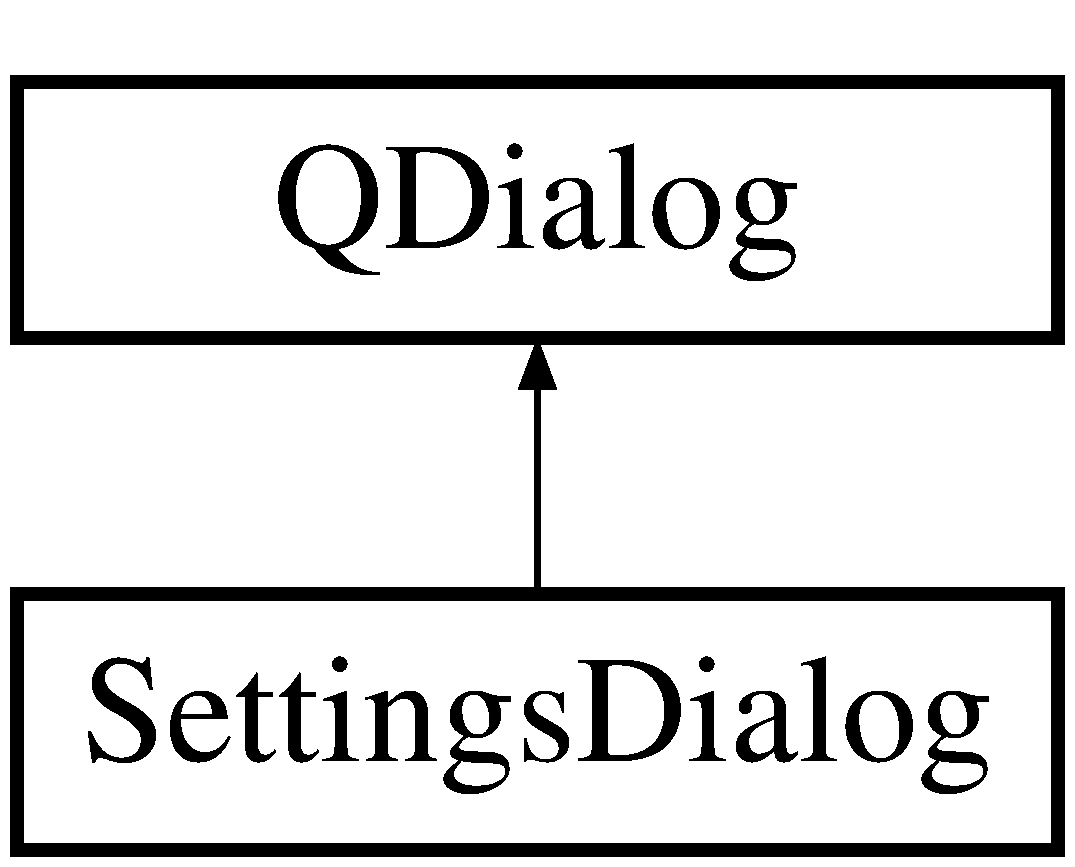
\includegraphics[height=2.000000cm]{class_settings_dialog}
\end{center}
\end{figure}
\subsection*{Public Member Functions}
\begin{DoxyCompactItemize}
\item 
\hyperlink{class_settings_dialog_a50d64f2aa1317e9b10bd2ea1a6c011bb}{Settings\+Dialog} (const Q\+List$<$ Q\+Audio\+Device\+Info $>$ \&available\+Input\+Devices, const Q\+List$<$ Q\+Audio\+Device\+Info $>$ \&available\+Output\+Devices, Q\+Widget $\ast$parent=0)
\item 
\hyperlink{class_settings_dialog_ac48f54d4472902be0a3845a69167f068}{$\sim$\+Settings\+Dialog} ()
\item 
\hyperlink{spectrum_8h_adae4545e1609513867a86cc5e91fc1d4}{Window\+Function} \hyperlink{class_settings_dialog_a6cd9e3f301ccfa292d4205b20944aae0}{window\+Function} () const
\item 
const Q\+Audio\+Device\+Info \& \hyperlink{class_settings_dialog_a40d1decb770fb1fa322bd6e11ed3805f}{input\+Device} () const
\item 
const Q\+Audio\+Device\+Info \& \hyperlink{class_settings_dialog_afa48fa56f44b1e81def1ef936a35ed2f}{output\+Device} () const
\end{DoxyCompactItemize}


\subsection{Detailed Description}
Dialog used to control settings such as the audio input / output device and the windowing function. 

\subsection{Constructor \& Destructor Documentation}
\hypertarget{class_settings_dialog_a50d64f2aa1317e9b10bd2ea1a6c011bb}{}\label{class_settings_dialog_a50d64f2aa1317e9b10bd2ea1a6c011bb} 
\index{Settings\+Dialog@{Settings\+Dialog}!Settings\+Dialog@{Settings\+Dialog}}
\index{Settings\+Dialog@{Settings\+Dialog}!Settings\+Dialog@{Settings\+Dialog}}
\subsubsection{\texorpdfstring{Settings\+Dialog()}{SettingsDialog()}}
{\footnotesize\ttfamily Settings\+Dialog\+::\+Settings\+Dialog (\begin{DoxyParamCaption}\item[{const Q\+List$<$ Q\+Audio\+Device\+Info $>$ \&}]{available\+Input\+Devices,  }\item[{const Q\+List$<$ Q\+Audio\+Device\+Info $>$ \&}]{available\+Output\+Devices,  }\item[{Q\+Widget $\ast$}]{parent = {\ttfamily 0} }\end{DoxyParamCaption})}

\hypertarget{class_settings_dialog_ac48f54d4472902be0a3845a69167f068}{}\label{class_settings_dialog_ac48f54d4472902be0a3845a69167f068} 
\index{Settings\+Dialog@{Settings\+Dialog}!````~Settings\+Dialog@{$\sim$\+Settings\+Dialog}}
\index{````~Settings\+Dialog@{$\sim$\+Settings\+Dialog}!Settings\+Dialog@{Settings\+Dialog}}
\subsubsection{\texorpdfstring{$\sim$\+Settings\+Dialog()}{~SettingsDialog()}}
{\footnotesize\ttfamily Settings\+Dialog\+::$\sim$\+Settings\+Dialog (\begin{DoxyParamCaption}{ }\end{DoxyParamCaption})}



\subsection{Member Function Documentation}
\hypertarget{class_settings_dialog_a40d1decb770fb1fa322bd6e11ed3805f}{}\label{class_settings_dialog_a40d1decb770fb1fa322bd6e11ed3805f} 
\index{Settings\+Dialog@{Settings\+Dialog}!input\+Device@{input\+Device}}
\index{input\+Device@{input\+Device}!Settings\+Dialog@{Settings\+Dialog}}
\subsubsection{\texorpdfstring{input\+Device()}{inputDevice()}}
{\footnotesize\ttfamily const Q\+Audio\+Device\+Info\& Settings\+Dialog\+::input\+Device (\begin{DoxyParamCaption}{ }\end{DoxyParamCaption}) const\hspace{0.3cm}{\ttfamily [inline]}}

\hypertarget{class_settings_dialog_afa48fa56f44b1e81def1ef936a35ed2f}{}\label{class_settings_dialog_afa48fa56f44b1e81def1ef936a35ed2f} 
\index{Settings\+Dialog@{Settings\+Dialog}!output\+Device@{output\+Device}}
\index{output\+Device@{output\+Device}!Settings\+Dialog@{Settings\+Dialog}}
\subsubsection{\texorpdfstring{output\+Device()}{outputDevice()}}
{\footnotesize\ttfamily const Q\+Audio\+Device\+Info\& Settings\+Dialog\+::output\+Device (\begin{DoxyParamCaption}{ }\end{DoxyParamCaption}) const\hspace{0.3cm}{\ttfamily [inline]}}

\hypertarget{class_settings_dialog_a6cd9e3f301ccfa292d4205b20944aae0}{}\label{class_settings_dialog_a6cd9e3f301ccfa292d4205b20944aae0} 
\index{Settings\+Dialog@{Settings\+Dialog}!window\+Function@{window\+Function}}
\index{window\+Function@{window\+Function}!Settings\+Dialog@{Settings\+Dialog}}
\subsubsection{\texorpdfstring{window\+Function()}{windowFunction()}}
{\footnotesize\ttfamily \hyperlink{spectrum_8h_adae4545e1609513867a86cc5e91fc1d4}{Window\+Function} Settings\+Dialog\+::window\+Function (\begin{DoxyParamCaption}{ }\end{DoxyParamCaption}) const\hspace{0.3cm}{\ttfamily [inline]}}



The documentation for this class was generated from the following files\+:\begin{DoxyCompactItemize}
\item 
app/\hyperlink{settingsdialog_8h}{settingsdialog.\+h}\item 
app/\hyperlink{settingsdialog_8cpp}{settingsdialog.\+cpp}\end{DoxyCompactItemize}

\hypertarget{class_spectrograph}{}\section{Spectrograph Class Reference}
\label{class_spectrograph}\index{Spectrograph@{Spectrograph}}


{\ttfamily \#include $<$spectrograph.\+h$>$}

Inheritance diagram for Spectrograph\+:\begin{figure}[H]
\begin{center}
\leavevmode
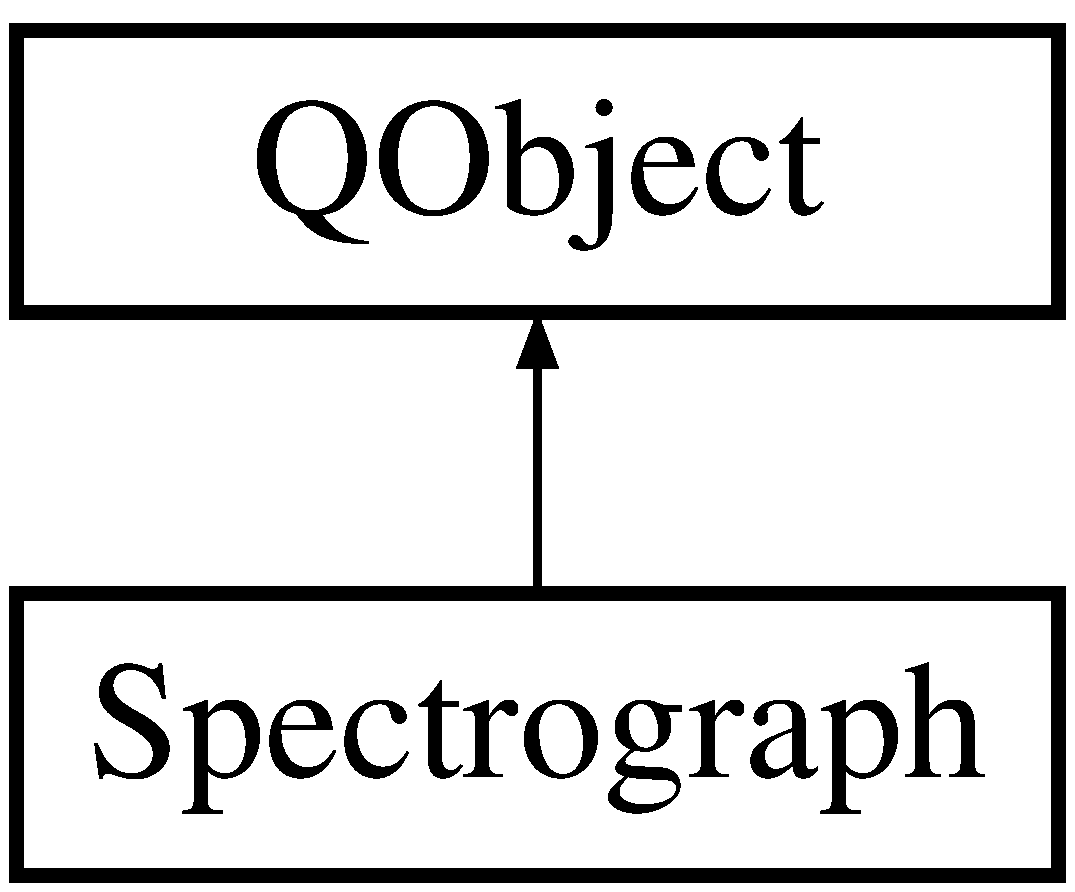
\includegraphics[height=2.000000cm]{class_spectrograph}
\end{center}
\end{figure}
\subsection*{Public Slots}
\begin{DoxyCompactItemize}
\item 
void \hyperlink{class_spectrograph_a63c0355273ab24b5206817695421747d}{reset} ()
\item 
void \hyperlink{class_spectrograph_af9cdafaa2e367c697a253a66e25c62a4}{spectrum\+Changed} (const \hyperlink{class_frequency_spectrum}{Frequency\+Spectrum} \&spectrum)
\item 
void \hyperlink{class_spectrograph_a3c6f5ae666d675d0326271511b38f4a2}{set\+Window\+Function} (\hyperlink{spectrum_8h_adae4545e1609513867a86cc5e91fc1d4}{Window\+Function} type)
\item 
void \hyperlink{class_spectrograph_aec6520868d48dc83485d6716b977f65b}{calculate\+Spectrum} (Q\+Byte\+Array \&m\+\_\+buffer, qint64 position)
\item 
void \hyperlink{class_spectrograph_ae267e7e06cb7eaec965150a73c21e4ce}{set\+Format} (const Q\+Audio\+Format \&format)
\item 
void \hyperlink{class_spectrograph_af6a83c1feec2657104a983ae334ceae3}{buffer\+Changed} (qint64 position, qint64 length, const Q\+Byte\+Array \&buffer)
\item 
void \hyperlink{class_spectrograph_a94b5df4c4d57b03cc588b2ecfc0d9596}{subsctibe\+Chart} (Q\+X\+Y\+Series $\ast$set)
\item 
void \hyperlink{class_spectrograph_a6c5811644f0e182a7814027f7d9b702c}{un\+Subsctibe\+Chart} (Q\+X\+Y\+Series $\ast$set)
\item 
int \hyperlink{class_spectrograph_a4a7f2b78c288816942356f2452166211}{get\+Bar\+Number} ()
\end{DoxyCompactItemize}
\subsection*{Signals}
\begin{DoxyCompactItemize}
\item 
void \hyperlink{class_spectrograph_a1046b17fbd22d0724f06d461acb77bef}{info\+Message} (const Q\+String \&message, int interval\+Ms)
\end{DoxyCompactItemize}
\subsection*{Public Member Functions}
\begin{DoxyCompactItemize}
\item 
\hyperlink{class_spectrograph_afcfc87c4b07094a705dabb1b43c366ee}{Spectrograph} (Q\+Object $\ast$parent=0)
\item 
\hyperlink{class_spectrograph_aede83dadf66ffca77b01b023ee35d8b6}{$\sim$\+Spectrograph} ()
\item 
void \hyperlink{class_spectrograph_a5eba417e888dc0871f5ad1348849b693}{set\+Params} (int num\+Bars, qreal low\+Freq, qreal high\+Freq)
\item 
void \hyperlink{class_spectrograph_a9141c4da693b8c00d4ab8d9b5ba6e670}{timer\+Event} (Q\+Timer\+Event $\ast$event)
\end{DoxyCompactItemize}


\subsection{Constructor \& Destructor Documentation}
\hypertarget{class_spectrograph_afcfc87c4b07094a705dabb1b43c366ee}{}\label{class_spectrograph_afcfc87c4b07094a705dabb1b43c366ee} 
\index{Spectrograph@{Spectrograph}!Spectrograph@{Spectrograph}}
\index{Spectrograph@{Spectrograph}!Spectrograph@{Spectrograph}}
\subsubsection{\texorpdfstring{Spectrograph()}{Spectrograph()}}
{\footnotesize\ttfamily Spectrograph\+::\+Spectrograph (\begin{DoxyParamCaption}\item[{Q\+Object $\ast$}]{parent = {\ttfamily 0} }\end{DoxyParamCaption})\hspace{0.3cm}{\ttfamily [explicit]}}

\hypertarget{class_spectrograph_aede83dadf66ffca77b01b023ee35d8b6}{}\label{class_spectrograph_aede83dadf66ffca77b01b023ee35d8b6} 
\index{Spectrograph@{Spectrograph}!````~Spectrograph@{$\sim$\+Spectrograph}}
\index{````~Spectrograph@{$\sim$\+Spectrograph}!Spectrograph@{Spectrograph}}
\subsubsection{\texorpdfstring{$\sim$\+Spectrograph()}{~Spectrograph()}}
{\footnotesize\ttfamily Spectrograph\+::$\sim$\+Spectrograph (\begin{DoxyParamCaption}{ }\end{DoxyParamCaption})}



\subsection{Member Function Documentation}
\hypertarget{class_spectrograph_af6a83c1feec2657104a983ae334ceae3}{}\label{class_spectrograph_af6a83c1feec2657104a983ae334ceae3} 
\index{Spectrograph@{Spectrograph}!buffer\+Changed@{buffer\+Changed}}
\index{buffer\+Changed@{buffer\+Changed}!Spectrograph@{Spectrograph}}
\subsubsection{\texorpdfstring{buffer\+Changed}{bufferChanged}}
{\footnotesize\ttfamily void Spectrograph\+::buffer\+Changed (\begin{DoxyParamCaption}\item[{qint64}]{position,  }\item[{qint64}]{length,  }\item[{const Q\+Byte\+Array \&}]{buffer }\end{DoxyParamCaption})\hspace{0.3cm}{\ttfamily [slot]}}

\hypertarget{class_spectrograph_aec6520868d48dc83485d6716b977f65b}{}\label{class_spectrograph_aec6520868d48dc83485d6716b977f65b} 
\index{Spectrograph@{Spectrograph}!calculate\+Spectrum@{calculate\+Spectrum}}
\index{calculate\+Spectrum@{calculate\+Spectrum}!Spectrograph@{Spectrograph}}
\subsubsection{\texorpdfstring{calculate\+Spectrum}{calculateSpectrum}}
{\footnotesize\ttfamily void Spectrograph\+::calculate\+Spectrum (\begin{DoxyParamCaption}\item[{Q\+Byte\+Array \&}]{m\+\_\+buffer,  }\item[{qint64}]{position }\end{DoxyParamCaption})\hspace{0.3cm}{\ttfamily [slot]}}

\hypertarget{class_spectrograph_a4a7f2b78c288816942356f2452166211}{}\label{class_spectrograph_a4a7f2b78c288816942356f2452166211} 
\index{Spectrograph@{Spectrograph}!get\+Bar\+Number@{get\+Bar\+Number}}
\index{get\+Bar\+Number@{get\+Bar\+Number}!Spectrograph@{Spectrograph}}
\subsubsection{\texorpdfstring{get\+Bar\+Number}{getBarNumber}}
{\footnotesize\ttfamily int Spectrograph\+::get\+Bar\+Number (\begin{DoxyParamCaption}{ }\end{DoxyParamCaption})\hspace{0.3cm}{\ttfamily [slot]}}

\hypertarget{class_spectrograph_a1046b17fbd22d0724f06d461acb77bef}{}\label{class_spectrograph_a1046b17fbd22d0724f06d461acb77bef} 
\index{Spectrograph@{Spectrograph}!info\+Message@{info\+Message}}
\index{info\+Message@{info\+Message}!Spectrograph@{Spectrograph}}
\subsubsection{\texorpdfstring{info\+Message}{infoMessage}}
{\footnotesize\ttfamily void Spectrograph\+::info\+Message (\begin{DoxyParamCaption}\item[{const Q\+String \&}]{message,  }\item[{int}]{interval\+Ms }\end{DoxyParamCaption})\hspace{0.3cm}{\ttfamily [signal]}}

\hypertarget{class_spectrograph_a63c0355273ab24b5206817695421747d}{}\label{class_spectrograph_a63c0355273ab24b5206817695421747d} 
\index{Spectrograph@{Spectrograph}!reset@{reset}}
\index{reset@{reset}!Spectrograph@{Spectrograph}}
\subsubsection{\texorpdfstring{reset}{reset}}
{\footnotesize\ttfamily void Spectrograph\+::reset (\begin{DoxyParamCaption}{ }\end{DoxyParamCaption})\hspace{0.3cm}{\ttfamily [slot]}}

\hypertarget{class_spectrograph_ae267e7e06cb7eaec965150a73c21e4ce}{}\label{class_spectrograph_ae267e7e06cb7eaec965150a73c21e4ce} 
\index{Spectrograph@{Spectrograph}!set\+Format@{set\+Format}}
\index{set\+Format@{set\+Format}!Spectrograph@{Spectrograph}}
\subsubsection{\texorpdfstring{set\+Format}{setFormat}}
{\footnotesize\ttfamily void Spectrograph\+::set\+Format (\begin{DoxyParamCaption}\item[{const Q\+Audio\+Format \&}]{format }\end{DoxyParamCaption})\hspace{0.3cm}{\ttfamily [slot]}}

\hypertarget{class_spectrograph_a5eba417e888dc0871f5ad1348849b693}{}\label{class_spectrograph_a5eba417e888dc0871f5ad1348849b693} 
\index{Spectrograph@{Spectrograph}!set\+Params@{set\+Params}}
\index{set\+Params@{set\+Params}!Spectrograph@{Spectrograph}}
\subsubsection{\texorpdfstring{set\+Params()}{setParams()}}
{\footnotesize\ttfamily void Spectrograph\+::set\+Params (\begin{DoxyParamCaption}\item[{int}]{num\+Bars,  }\item[{qreal}]{low\+Freq,  }\item[{qreal}]{high\+Freq }\end{DoxyParamCaption})}

reinit list \hypertarget{class_spectrograph_a3c6f5ae666d675d0326271511b38f4a2}{}\label{class_spectrograph_a3c6f5ae666d675d0326271511b38f4a2} 
\index{Spectrograph@{Spectrograph}!set\+Window\+Function@{set\+Window\+Function}}
\index{set\+Window\+Function@{set\+Window\+Function}!Spectrograph@{Spectrograph}}
\subsubsection{\texorpdfstring{set\+Window\+Function}{setWindowFunction}}
{\footnotesize\ttfamily void Spectrograph\+::set\+Window\+Function (\begin{DoxyParamCaption}\item[{\hyperlink{spectrum_8h_adae4545e1609513867a86cc5e91fc1d4}{Window\+Function}}]{type }\end{DoxyParamCaption})\hspace{0.3cm}{\ttfamily [slot]}}

\hypertarget{class_spectrograph_af9cdafaa2e367c697a253a66e25c62a4}{}\label{class_spectrograph_af9cdafaa2e367c697a253a66e25c62a4} 
\index{Spectrograph@{Spectrograph}!spectrum\+Changed@{spectrum\+Changed}}
\index{spectrum\+Changed@{spectrum\+Changed}!Spectrograph@{Spectrograph}}
\subsubsection{\texorpdfstring{spectrum\+Changed}{spectrumChanged}}
{\footnotesize\ttfamily void Spectrograph\+::spectrum\+Changed (\begin{DoxyParamCaption}\item[{const \hyperlink{class_frequency_spectrum}{Frequency\+Spectrum} \&}]{spectrum }\end{DoxyParamCaption})\hspace{0.3cm}{\ttfamily [slot]}}

\hypertarget{class_spectrograph_a94b5df4c4d57b03cc588b2ecfc0d9596}{}\label{class_spectrograph_a94b5df4c4d57b03cc588b2ecfc0d9596} 
\index{Spectrograph@{Spectrograph}!subsctibe\+Chart@{subsctibe\+Chart}}
\index{subsctibe\+Chart@{subsctibe\+Chart}!Spectrograph@{Spectrograph}}
\subsubsection{\texorpdfstring{subsctibe\+Chart}{subsctibeChart}}
{\footnotesize\ttfamily void Spectrograph\+::subsctibe\+Chart (\begin{DoxyParamCaption}\item[{Q\+X\+Y\+Series $\ast$}]{set }\end{DoxyParamCaption})\hspace{0.3cm}{\ttfamily [slot]}}

\hypertarget{class_spectrograph_a9141c4da693b8c00d4ab8d9b5ba6e670}{}\label{class_spectrograph_a9141c4da693b8c00d4ab8d9b5ba6e670} 
\index{Spectrograph@{Spectrograph}!timer\+Event@{timer\+Event}}
\index{timer\+Event@{timer\+Event}!Spectrograph@{Spectrograph}}
\subsubsection{\texorpdfstring{timer\+Event()}{timerEvent()}}
{\footnotesize\ttfamily void Spectrograph\+::timer\+Event (\begin{DoxyParamCaption}\item[{Q\+Timer\+Event $\ast$}]{event }\end{DoxyParamCaption})}

\hypertarget{class_spectrograph_a6c5811644f0e182a7814027f7d9b702c}{}\label{class_spectrograph_a6c5811644f0e182a7814027f7d9b702c} 
\index{Spectrograph@{Spectrograph}!un\+Subsctibe\+Chart@{un\+Subsctibe\+Chart}}
\index{un\+Subsctibe\+Chart@{un\+Subsctibe\+Chart}!Spectrograph@{Spectrograph}}
\subsubsection{\texorpdfstring{un\+Subsctibe\+Chart}{unSubsctibeChart}}
{\footnotesize\ttfamily void Spectrograph\+::un\+Subsctibe\+Chart (\begin{DoxyParamCaption}\item[{Q\+X\+Y\+Series $\ast$}]{set }\end{DoxyParamCaption})\hspace{0.3cm}{\ttfamily [slot]}}



The documentation for this class was generated from the following files\+:\begin{DoxyCompactItemize}
\item 
app/\hyperlink{spectrograph_8h}{spectrograph.\+h}\item 
app/\hyperlink{spectrograph_8cpp}{spectrograph.\+cpp}\end{DoxyCompactItemize}

\hypertarget{class_spectrum_analyser}{}\section{Spectrum\+Analyser Class Reference}
\label{class_spectrum_analyser}\index{Spectrum\+Analyser@{Spectrum\+Analyser}}


{\ttfamily \#include $<$spectrumanalyser.\+h$>$}

Inheritance diagram for Spectrum\+Analyser\+:\begin{figure}[H]
\begin{center}
\leavevmode
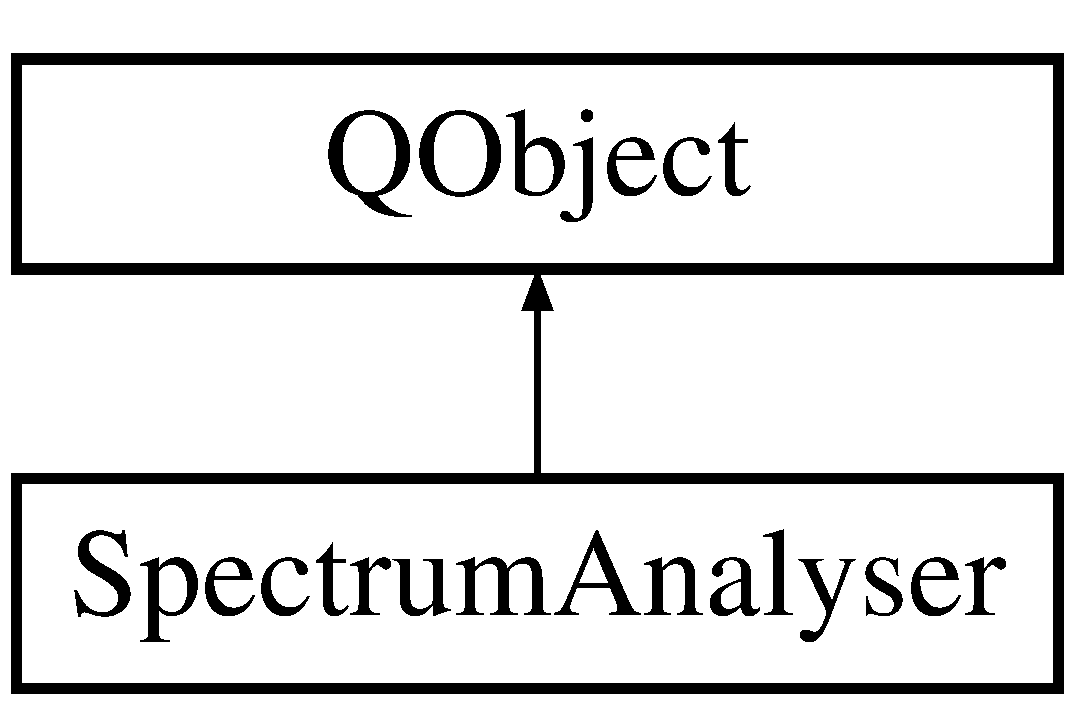
\includegraphics[height=2.000000cm]{class_spectrum_analyser}
\end{center}
\end{figure}
\subsection*{Signals}
\begin{DoxyCompactItemize}
\item 
void \hyperlink{class_spectrum_analyser_af2dd8d387193fa6743ac15d3f8163ee0}{spectrum\+Changed} (const \hyperlink{class_frequency_spectrum}{Frequency\+Spectrum} \&spectrum)
\end{DoxyCompactItemize}
\subsection*{Public Member Functions}
\begin{DoxyCompactItemize}
\item 
\hyperlink{class_spectrum_analyser_abf706ac78327bc590b90b586086c0cd5}{Spectrum\+Analyser} (Q\+Object $\ast$parent=0)
\item 
\hyperlink{class_spectrum_analyser_a3737f48dd1d95b09aeeaf3e1f081591e}{$\sim$\+Spectrum\+Analyser} ()
\item 
void \hyperlink{class_spectrum_analyser_a6aeb6c39dd89dd5c5881198ae413ec74}{set\+Window\+Function} (\hyperlink{spectrum_8h_adae4545e1609513867a86cc5e91fc1d4}{Window\+Function} type)
\item 
void \hyperlink{class_spectrum_analyser_aecd698124fcdd83760b9e808f003e1a6}{calculate} (const Q\+Byte\+Array \&buffer, const Q\+Audio\+Format \&format)
\item 
bool \hyperlink{class_spectrum_analyser_acac3bd1ac5fc255c01ea0288e50fee6c}{is\+Ready} () const
\item 
void \hyperlink{class_spectrum_analyser_a1ed17c67c3676facec7e987512eaa962}{cancel\+Calculation} ()
\end{DoxyCompactItemize}


\subsection{Detailed Description}
Class which performs frequency spectrum analysis on a window of audio samples, provided to it by the \hyperlink{class_engine}{Engine}. 

\subsection{Constructor \& Destructor Documentation}
\hypertarget{class_spectrum_analyser_abf706ac78327bc590b90b586086c0cd5}{}\label{class_spectrum_analyser_abf706ac78327bc590b90b586086c0cd5} 
\index{Spectrum\+Analyser@{Spectrum\+Analyser}!Spectrum\+Analyser@{Spectrum\+Analyser}}
\index{Spectrum\+Analyser@{Spectrum\+Analyser}!Spectrum\+Analyser@{Spectrum\+Analyser}}
\subsubsection{\texorpdfstring{Spectrum\+Analyser()}{SpectrumAnalyser()}}
{\footnotesize\ttfamily Spectrum\+Analyser\+::\+Spectrum\+Analyser (\begin{DoxyParamCaption}\item[{Q\+Object $\ast$}]{parent = {\ttfamily 0} }\end{DoxyParamCaption})}

\hypertarget{class_spectrum_analyser_a3737f48dd1d95b09aeeaf3e1f081591e}{}\label{class_spectrum_analyser_a3737f48dd1d95b09aeeaf3e1f081591e} 
\index{Spectrum\+Analyser@{Spectrum\+Analyser}!````~Spectrum\+Analyser@{$\sim$\+Spectrum\+Analyser}}
\index{````~Spectrum\+Analyser@{$\sim$\+Spectrum\+Analyser}!Spectrum\+Analyser@{Spectrum\+Analyser}}
\subsubsection{\texorpdfstring{$\sim$\+Spectrum\+Analyser()}{~SpectrumAnalyser()}}
{\footnotesize\ttfamily Spectrum\+Analyser\+::$\sim$\+Spectrum\+Analyser (\begin{DoxyParamCaption}{ }\end{DoxyParamCaption})}



\subsection{Member Function Documentation}
\hypertarget{class_spectrum_analyser_aecd698124fcdd83760b9e808f003e1a6}{}\label{class_spectrum_analyser_aecd698124fcdd83760b9e808f003e1a6} 
\index{Spectrum\+Analyser@{Spectrum\+Analyser}!calculate@{calculate}}
\index{calculate@{calculate}!Spectrum\+Analyser@{Spectrum\+Analyser}}
\subsubsection{\texorpdfstring{calculate()}{calculate()}}
{\footnotesize\ttfamily void Spectrum\+Analyser\+::calculate (\begin{DoxyParamCaption}\item[{const Q\+Byte\+Array \&}]{buffer,  }\item[{const Q\+Audio\+Format \&}]{format }\end{DoxyParamCaption})}

\hypertarget{class_spectrum_analyser_a1ed17c67c3676facec7e987512eaa962}{}\label{class_spectrum_analyser_a1ed17c67c3676facec7e987512eaa962} 
\index{Spectrum\+Analyser@{Spectrum\+Analyser}!cancel\+Calculation@{cancel\+Calculation}}
\index{cancel\+Calculation@{cancel\+Calculation}!Spectrum\+Analyser@{Spectrum\+Analyser}}
\subsubsection{\texorpdfstring{cancel\+Calculation()}{cancelCalculation()}}
{\footnotesize\ttfamily void Spectrum\+Analyser\+::cancel\+Calculation (\begin{DoxyParamCaption}{ }\end{DoxyParamCaption})}

\hypertarget{class_spectrum_analyser_acac3bd1ac5fc255c01ea0288e50fee6c}{}\label{class_spectrum_analyser_acac3bd1ac5fc255c01ea0288e50fee6c} 
\index{Spectrum\+Analyser@{Spectrum\+Analyser}!is\+Ready@{is\+Ready}}
\index{is\+Ready@{is\+Ready}!Spectrum\+Analyser@{Spectrum\+Analyser}}
\subsubsection{\texorpdfstring{is\+Ready()}{isReady()}}
{\footnotesize\ttfamily bool Spectrum\+Analyser\+::is\+Ready (\begin{DoxyParamCaption}{ }\end{DoxyParamCaption}) const}

\hypertarget{class_spectrum_analyser_a6aeb6c39dd89dd5c5881198ae413ec74}{}\label{class_spectrum_analyser_a6aeb6c39dd89dd5c5881198ae413ec74} 
\index{Spectrum\+Analyser@{Spectrum\+Analyser}!set\+Window\+Function@{set\+Window\+Function}}
\index{set\+Window\+Function@{set\+Window\+Function}!Spectrum\+Analyser@{Spectrum\+Analyser}}
\subsubsection{\texorpdfstring{set\+Window\+Function()}{setWindowFunction()}}
{\footnotesize\ttfamily void Spectrum\+Analyser\+::set\+Window\+Function (\begin{DoxyParamCaption}\item[{\hyperlink{spectrum_8h_adae4545e1609513867a86cc5e91fc1d4}{Window\+Function}}]{type }\end{DoxyParamCaption})}

\hypertarget{class_spectrum_analyser_af2dd8d387193fa6743ac15d3f8163ee0}{}\label{class_spectrum_analyser_af2dd8d387193fa6743ac15d3f8163ee0} 
\index{Spectrum\+Analyser@{Spectrum\+Analyser}!spectrum\+Changed@{spectrum\+Changed}}
\index{spectrum\+Changed@{spectrum\+Changed}!Spectrum\+Analyser@{Spectrum\+Analyser}}
\subsubsection{\texorpdfstring{spectrum\+Changed}{spectrumChanged}}
{\footnotesize\ttfamily void Spectrum\+Analyser\+::spectrum\+Changed (\begin{DoxyParamCaption}\item[{const \hyperlink{class_frequency_spectrum}{Frequency\+Spectrum} \&}]{spectrum }\end{DoxyParamCaption})\hspace{0.3cm}{\ttfamily [signal]}}



The documentation for this class was generated from the following files\+:\begin{DoxyCompactItemize}
\item 
app/\hyperlink{spectrumanalyser_8h}{spectrumanalyser.\+h}\item 
app/\hyperlink{spectrumanalyser_8cpp}{spectrumanalyser.\+cpp}\end{DoxyCompactItemize}

\hypertarget{class_spectrum_analyser_thread}{}\section{Spectrum\+Analyser\+Thread Class Reference}
\label{class_spectrum_analyser_thread}\index{Spectrum\+Analyser\+Thread@{Spectrum\+Analyser\+Thread}}


{\ttfamily \#include $<$spectrumanalyser.\+h$>$}

Inheritance diagram for Spectrum\+Analyser\+Thread\+:\begin{figure}[H]
\begin{center}
\leavevmode
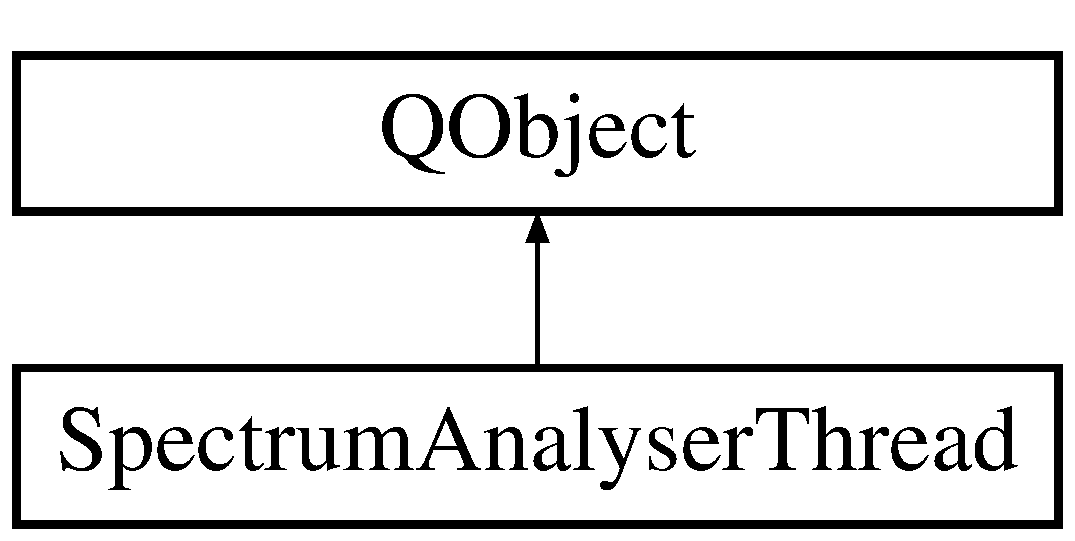
\includegraphics[height=2.000000cm]{class_spectrum_analyser_thread}
\end{center}
\end{figure}
\subsection*{Public Slots}
\begin{DoxyCompactItemize}
\item 
void \hyperlink{class_spectrum_analyser_thread_a823681736ef2719fbb6aec132a75b6cb}{set\+Window\+Function} (\hyperlink{spectrum_8h_adae4545e1609513867a86cc5e91fc1d4}{Window\+Function} type)
\item 
void \hyperlink{class_spectrum_analyser_thread_a6dc32705bf41e75f8d16f9c27bd2ee65}{calculate\+Spectrum} (const Q\+Byte\+Array \&buffer, int input\+Frequency, int bytes\+Per\+Sample)
\end{DoxyCompactItemize}
\subsection*{Signals}
\begin{DoxyCompactItemize}
\item 
void \hyperlink{class_spectrum_analyser_thread_adb2c9b6a5e017cd0805dac29c754b7f0}{calculation\+Complete} (const \hyperlink{class_frequency_spectrum}{Frequency\+Spectrum} \&spectrum)
\end{DoxyCompactItemize}
\subsection*{Public Member Functions}
\begin{DoxyCompactItemize}
\item 
\hyperlink{class_spectrum_analyser_thread_a35109a92c671b97f2cdaef0dcc5ab6c2}{Spectrum\+Analyser\+Thread} (Q\+Object $\ast$parent)
\item 
\hyperlink{class_spectrum_analyser_thread_a5d8f22dd659e87447f29bb7271a5f289}{$\sim$\+Spectrum\+Analyser\+Thread} ()
\end{DoxyCompactItemize}


\subsection{Detailed Description}
Implementation of the spectrum analysis which can be run in a separate thread. 

\subsection{Constructor \& Destructor Documentation}
\hypertarget{class_spectrum_analyser_thread_a35109a92c671b97f2cdaef0dcc5ab6c2}{}\label{class_spectrum_analyser_thread_a35109a92c671b97f2cdaef0dcc5ab6c2} 
\index{Spectrum\+Analyser\+Thread@{Spectrum\+Analyser\+Thread}!Spectrum\+Analyser\+Thread@{Spectrum\+Analyser\+Thread}}
\index{Spectrum\+Analyser\+Thread@{Spectrum\+Analyser\+Thread}!Spectrum\+Analyser\+Thread@{Spectrum\+Analyser\+Thread}}
\subsubsection{\texorpdfstring{Spectrum\+Analyser\+Thread()}{SpectrumAnalyserThread()}}
{\footnotesize\ttfamily Spectrum\+Analyser\+Thread\+::\+Spectrum\+Analyser\+Thread (\begin{DoxyParamCaption}\item[{Q\+Object $\ast$}]{parent }\end{DoxyParamCaption})}

\hypertarget{class_spectrum_analyser_thread_a5d8f22dd659e87447f29bb7271a5f289}{}\label{class_spectrum_analyser_thread_a5d8f22dd659e87447f29bb7271a5f289} 
\index{Spectrum\+Analyser\+Thread@{Spectrum\+Analyser\+Thread}!````~Spectrum\+Analyser\+Thread@{$\sim$\+Spectrum\+Analyser\+Thread}}
\index{````~Spectrum\+Analyser\+Thread@{$\sim$\+Spectrum\+Analyser\+Thread}!Spectrum\+Analyser\+Thread@{Spectrum\+Analyser\+Thread}}
\subsubsection{\texorpdfstring{$\sim$\+Spectrum\+Analyser\+Thread()}{~SpectrumAnalyserThread()}}
{\footnotesize\ttfamily Spectrum\+Analyser\+Thread\+::$\sim$\+Spectrum\+Analyser\+Thread (\begin{DoxyParamCaption}{ }\end{DoxyParamCaption})}



\subsection{Member Function Documentation}
\hypertarget{class_spectrum_analyser_thread_a6dc32705bf41e75f8d16f9c27bd2ee65}{}\label{class_spectrum_analyser_thread_a6dc32705bf41e75f8d16f9c27bd2ee65} 
\index{Spectrum\+Analyser\+Thread@{Spectrum\+Analyser\+Thread}!calculate\+Spectrum@{calculate\+Spectrum}}
\index{calculate\+Spectrum@{calculate\+Spectrum}!Spectrum\+Analyser\+Thread@{Spectrum\+Analyser\+Thread}}
\subsubsection{\texorpdfstring{calculate\+Spectrum}{calculateSpectrum}}
{\footnotesize\ttfamily void Spectrum\+Analyser\+Thread\+::calculate\+Spectrum (\begin{DoxyParamCaption}\item[{const Q\+Byte\+Array \&}]{buffer,  }\item[{int}]{input\+Frequency,  }\item[{int}]{bytes\+Per\+Sample }\end{DoxyParamCaption})\hspace{0.3cm}{\ttfamily [slot]}}

\hypertarget{class_spectrum_analyser_thread_adb2c9b6a5e017cd0805dac29c754b7f0}{}\label{class_spectrum_analyser_thread_adb2c9b6a5e017cd0805dac29c754b7f0} 
\index{Spectrum\+Analyser\+Thread@{Spectrum\+Analyser\+Thread}!calculation\+Complete@{calculation\+Complete}}
\index{calculation\+Complete@{calculation\+Complete}!Spectrum\+Analyser\+Thread@{Spectrum\+Analyser\+Thread}}
\subsubsection{\texorpdfstring{calculation\+Complete}{calculationComplete}}
{\footnotesize\ttfamily void Spectrum\+Analyser\+Thread\+::calculation\+Complete (\begin{DoxyParamCaption}\item[{const \hyperlink{class_frequency_spectrum}{Frequency\+Spectrum} \&}]{spectrum }\end{DoxyParamCaption})\hspace{0.3cm}{\ttfamily [signal]}}

\hypertarget{class_spectrum_analyser_thread_a823681736ef2719fbb6aec132a75b6cb}{}\label{class_spectrum_analyser_thread_a823681736ef2719fbb6aec132a75b6cb} 
\index{Spectrum\+Analyser\+Thread@{Spectrum\+Analyser\+Thread}!set\+Window\+Function@{set\+Window\+Function}}
\index{set\+Window\+Function@{set\+Window\+Function}!Spectrum\+Analyser\+Thread@{Spectrum\+Analyser\+Thread}}
\subsubsection{\texorpdfstring{set\+Window\+Function}{setWindowFunction}}
{\footnotesize\ttfamily void Spectrum\+Analyser\+Thread\+::set\+Window\+Function (\begin{DoxyParamCaption}\item[{\hyperlink{spectrum_8h_adae4545e1609513867a86cc5e91fc1d4}{Window\+Function}}]{type }\end{DoxyParamCaption})\hspace{0.3cm}{\ttfamily [slot]}}



The documentation for this class was generated from the following files\+:\begin{DoxyCompactItemize}
\item 
app/\hyperlink{spectrumanalyser_8h}{spectrumanalyser.\+h}\item 
app/\hyperlink{spectrumanalyser_8cpp}{spectrumanalyser.\+cpp}\end{DoxyCompactItemize}

\hypertarget{struct_swept_tone}{}\section{Swept\+Tone Struct Reference}
\label{struct_swept_tone}\index{Swept\+Tone@{Swept\+Tone}}


{\ttfamily \#include $<$spectrum.\+h$>$}

\subsection*{Public Member Functions}
\begin{DoxyCompactItemize}
\item 
\hyperlink{struct_swept_tone_a905368d1daa77ab33e190b5d47c26218}{Swept\+Tone} (qreal start=0.\+0, qreal end=0.\+0, qreal amp=0.\+0)
\item 
\hyperlink{struct_swept_tone_a79a1bcd511e7fc9b847603c4cefaa03c}{Swept\+Tone} (const \hyperlink{struct_tone}{Tone} \&tone)
\end{DoxyCompactItemize}
\subsection*{Public Attributes}
\begin{DoxyCompactItemize}
\item 
qreal \hyperlink{struct_swept_tone_acfccd7b4e61255b6061bb8151067db79}{start\+Freq}
\item 
qreal \hyperlink{struct_swept_tone_abad3f34970552d406721eb8c051911e5}{end\+Freq}
\item 
qreal \hyperlink{struct_swept_tone_a335b714b2688aa70154b736662b95d09}{amplitude}
\end{DoxyCompactItemize}


\subsection{Constructor \& Destructor Documentation}
\hypertarget{struct_swept_tone_a905368d1daa77ab33e190b5d47c26218}{}\label{struct_swept_tone_a905368d1daa77ab33e190b5d47c26218} 
\index{Swept\+Tone@{Swept\+Tone}!Swept\+Tone@{Swept\+Tone}}
\index{Swept\+Tone@{Swept\+Tone}!Swept\+Tone@{Swept\+Tone}}
\subsubsection{\texorpdfstring{Swept\+Tone()}{SweptTone()}\hspace{0.1cm}{\footnotesize\ttfamily [1/2]}}
{\footnotesize\ttfamily Swept\+Tone\+::\+Swept\+Tone (\begin{DoxyParamCaption}\item[{qreal}]{start = {\ttfamily 0.0},  }\item[{qreal}]{end = {\ttfamily 0.0},  }\item[{qreal}]{amp = {\ttfamily 0.0} }\end{DoxyParamCaption})\hspace{0.3cm}{\ttfamily [inline]}}

\hypertarget{struct_swept_tone_a79a1bcd511e7fc9b847603c4cefaa03c}{}\label{struct_swept_tone_a79a1bcd511e7fc9b847603c4cefaa03c} 
\index{Swept\+Tone@{Swept\+Tone}!Swept\+Tone@{Swept\+Tone}}
\index{Swept\+Tone@{Swept\+Tone}!Swept\+Tone@{Swept\+Tone}}
\subsubsection{\texorpdfstring{Swept\+Tone()}{SweptTone()}\hspace{0.1cm}{\footnotesize\ttfamily [2/2]}}
{\footnotesize\ttfamily Swept\+Tone\+::\+Swept\+Tone (\begin{DoxyParamCaption}\item[{const \hyperlink{struct_tone}{Tone} \&}]{tone }\end{DoxyParamCaption})\hspace{0.3cm}{\ttfamily [inline]}}



\subsection{Member Data Documentation}
\hypertarget{struct_swept_tone_a335b714b2688aa70154b736662b95d09}{}\label{struct_swept_tone_a335b714b2688aa70154b736662b95d09} 
\index{Swept\+Tone@{Swept\+Tone}!amplitude@{amplitude}}
\index{amplitude@{amplitude}!Swept\+Tone@{Swept\+Tone}}
\subsubsection{\texorpdfstring{amplitude}{amplitude}}
{\footnotesize\ttfamily qreal Swept\+Tone\+::amplitude}

\hypertarget{struct_swept_tone_abad3f34970552d406721eb8c051911e5}{}\label{struct_swept_tone_abad3f34970552d406721eb8c051911e5} 
\index{Swept\+Tone@{Swept\+Tone}!end\+Freq@{end\+Freq}}
\index{end\+Freq@{end\+Freq}!Swept\+Tone@{Swept\+Tone}}
\subsubsection{\texorpdfstring{end\+Freq}{endFreq}}
{\footnotesize\ttfamily qreal Swept\+Tone\+::end\+Freq}

\hypertarget{struct_swept_tone_acfccd7b4e61255b6061bb8151067db79}{}\label{struct_swept_tone_acfccd7b4e61255b6061bb8151067db79} 
\index{Swept\+Tone@{Swept\+Tone}!start\+Freq@{start\+Freq}}
\index{start\+Freq@{start\+Freq}!Swept\+Tone@{Swept\+Tone}}
\subsubsection{\texorpdfstring{start\+Freq}{startFreq}}
{\footnotesize\ttfamily qreal Swept\+Tone\+::start\+Freq}



The documentation for this struct was generated from the following file\+:\begin{DoxyCompactItemize}
\item 
app/\hyperlink{spectrum_8h}{spectrum.\+h}\end{DoxyCompactItemize}

\hypertarget{struct_tone}{}\section{Tone Struct Reference}
\label{struct_tone}\index{Tone@{Tone}}


{\ttfamily \#include $<$spectrum.\+h$>$}

\subsection*{Public Member Functions}
\begin{DoxyCompactItemize}
\item 
\hyperlink{struct_tone_a519be8e3fb9fd042aa3980006c888b4b}{Tone} (qreal freq=0.\+0, qreal amp=0.\+0)
\end{DoxyCompactItemize}
\subsection*{Public Attributes}
\begin{DoxyCompactItemize}
\item 
qreal \hyperlink{struct_tone_af9f6f7f70cd653e3a4033d1d9bb51657}{frequency}
\item 
qreal \hyperlink{struct_tone_a1652dad40126318d5bb4919c405a3a93}{amplitude}
\end{DoxyCompactItemize}


\subsection{Constructor \& Destructor Documentation}
\hypertarget{struct_tone_a519be8e3fb9fd042aa3980006c888b4b}{}\label{struct_tone_a519be8e3fb9fd042aa3980006c888b4b} 
\index{Tone@{Tone}!Tone@{Tone}}
\index{Tone@{Tone}!Tone@{Tone}}
\subsubsection{\texorpdfstring{Tone()}{Tone()}}
{\footnotesize\ttfamily Tone\+::\+Tone (\begin{DoxyParamCaption}\item[{qreal}]{freq = {\ttfamily 0.0},  }\item[{qreal}]{amp = {\ttfamily 0.0} }\end{DoxyParamCaption})\hspace{0.3cm}{\ttfamily [inline]}}



\subsection{Member Data Documentation}
\hypertarget{struct_tone_a1652dad40126318d5bb4919c405a3a93}{}\label{struct_tone_a1652dad40126318d5bb4919c405a3a93} 
\index{Tone@{Tone}!amplitude@{amplitude}}
\index{amplitude@{amplitude}!Tone@{Tone}}
\subsubsection{\texorpdfstring{amplitude}{amplitude}}
{\footnotesize\ttfamily qreal Tone\+::amplitude}

\hypertarget{struct_tone_af9f6f7f70cd653e3a4033d1d9bb51657}{}\label{struct_tone_af9f6f7f70cd653e3a4033d1d9bb51657} 
\index{Tone@{Tone}!frequency@{frequency}}
\index{frequency@{frequency}!Tone@{Tone}}
\subsubsection{\texorpdfstring{frequency}{frequency}}
{\footnotesize\ttfamily qreal Tone\+::frequency}



The documentation for this struct was generated from the following file\+:\begin{DoxyCompactItemize}
\item 
app/\hyperlink{spectrum_8h}{spectrum.\+h}\end{DoxyCompactItemize}

\hypertarget{class_waveform}{}\section{Waveform Class Reference}
\label{class_waveform}\index{Waveform@{Waveform}}


{\ttfamily \#include $<$waveform.\+h$>$}

Inheritance diagram for Waveform\+:\begin{figure}[H]
\begin{center}
\leavevmode
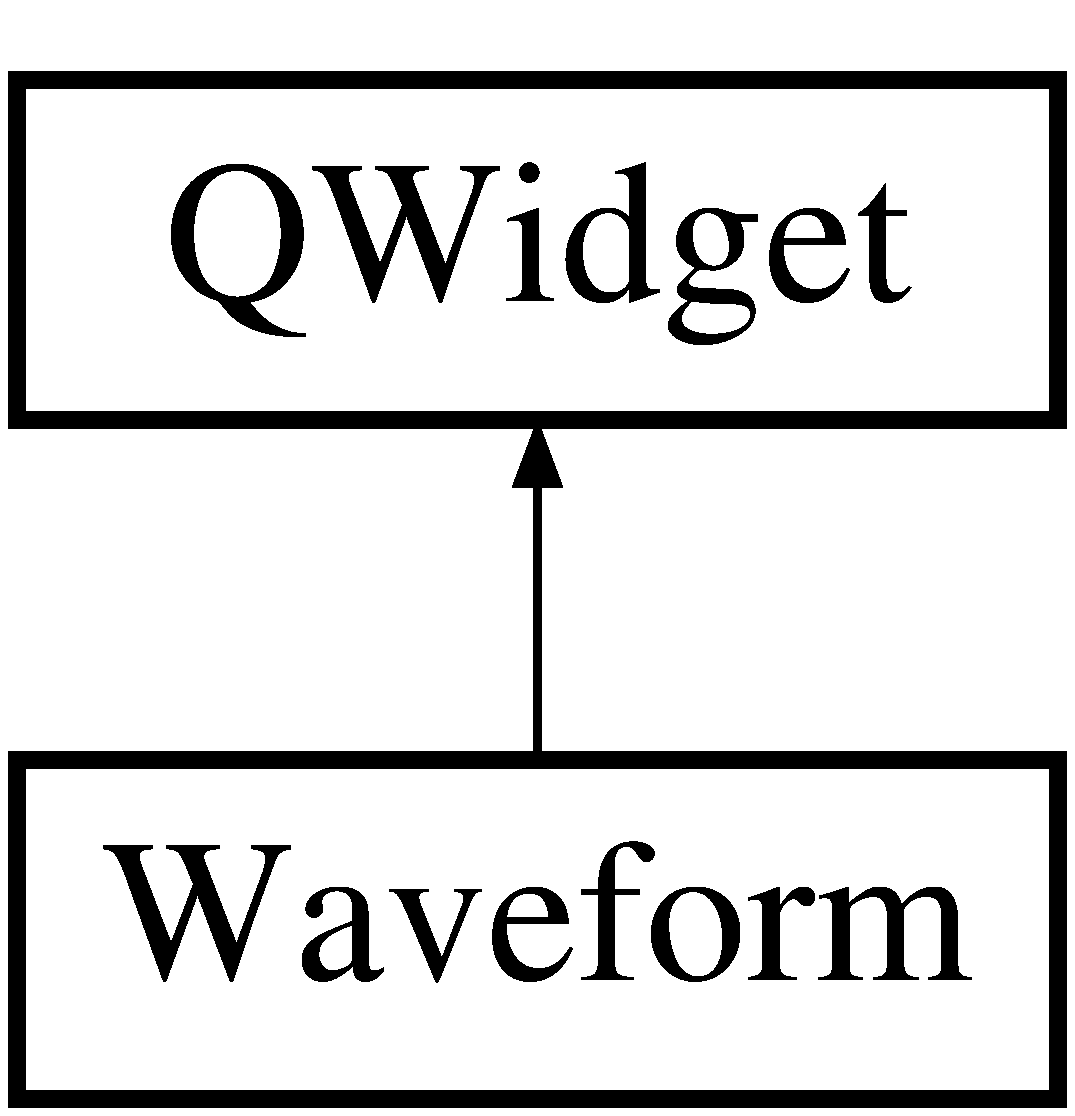
\includegraphics[height=2.000000cm]{class_waveform}
\end{center}
\end{figure}
\subsection*{Public Slots}
\begin{DoxyCompactItemize}
\item 
void \hyperlink{class_waveform_ae4dc908754aa8290280b60b14af11728}{buffer\+Changed} (qint64 position, qint64 length, const Q\+Byte\+Array \&buffer)
\item 
void \hyperlink{class_waveform_a3f6b6306fc0da548a763bf41d523fe28}{audio\+Position\+Changed} (qint64 position)
\end{DoxyCompactItemize}
\subsection*{Public Member Functions}
\begin{DoxyCompactItemize}
\item 
\hyperlink{class_waveform_a20e3236d7e3d215fcddd51062fcff350}{Waveform} (Q\+Widget $\ast$parent=0)
\item 
\hyperlink{class_waveform_af4f2ae8b1749306657602b53a8ab90df}{$\sim$\+Waveform} ()
\item 
void \hyperlink{class_waveform_a0c3a57dd99d9d203c1bfd846d639939f}{paint\+Event} (Q\+Paint\+Event $\ast$event)
\item 
void \hyperlink{class_waveform_a3d814bfdf6ec4d47e80e34685c2fa464}{resize\+Event} (Q\+Resize\+Event $\ast$event)
\item 
void \hyperlink{class_waveform_a0abffebbd2efcd6047137095f99a97f1}{initialize} (const Q\+Audio\+Format \&format, qint64 audio\+Buffer\+Size, qint64 window\+Duration\+Us)
\item 
void \hyperlink{class_waveform_ae97ba3abb25987f5df0b237850be5ec7}{reset} ()
\item 
void \hyperlink{class_waveform_aa57d2fa418d6ac920de5b81e8ec9e6fc}{set\+Auto\+Update\+Position} (bool enabled)
\end{DoxyCompactItemize}


\subsection{Detailed Description}
Widget which displays a section of the audio waveform.

The waveform is rendered on a set of Q\+Pixmaps which form a group of tiles whose extent covers the widget. As the audio position is updated, these tiles are scrolled from left to right; when the left-\/most tile scrolls outside the widget, it is moved to the right end of the tile array and painted with the next section of the waveform. 

\subsection{Constructor \& Destructor Documentation}
\hypertarget{class_waveform_a20e3236d7e3d215fcddd51062fcff350}{}\label{class_waveform_a20e3236d7e3d215fcddd51062fcff350} 
\index{Waveform@{Waveform}!Waveform@{Waveform}}
\index{Waveform@{Waveform}!Waveform@{Waveform}}
\subsubsection{\texorpdfstring{Waveform()}{Waveform()}}
{\footnotesize\ttfamily Waveform\+::\+Waveform (\begin{DoxyParamCaption}\item[{Q\+Widget $\ast$}]{parent = {\ttfamily 0} }\end{DoxyParamCaption})\hspace{0.3cm}{\ttfamily [explicit]}}

\hypertarget{class_waveform_af4f2ae8b1749306657602b53a8ab90df}{}\label{class_waveform_af4f2ae8b1749306657602b53a8ab90df} 
\index{Waveform@{Waveform}!````~Waveform@{$\sim$\+Waveform}}
\index{````~Waveform@{$\sim$\+Waveform}!Waveform@{Waveform}}
\subsubsection{\texorpdfstring{$\sim$\+Waveform()}{~Waveform()}}
{\footnotesize\ttfamily Waveform\+::$\sim$\+Waveform (\begin{DoxyParamCaption}{ }\end{DoxyParamCaption})}



\subsection{Member Function Documentation}
\hypertarget{class_waveform_a3f6b6306fc0da548a763bf41d523fe28}{}\label{class_waveform_a3f6b6306fc0da548a763bf41d523fe28} 
\index{Waveform@{Waveform}!audio\+Position\+Changed@{audio\+Position\+Changed}}
\index{audio\+Position\+Changed@{audio\+Position\+Changed}!Waveform@{Waveform}}
\subsubsection{\texorpdfstring{audio\+Position\+Changed}{audioPositionChanged}}
{\footnotesize\ttfamily void Waveform\+::audio\+Position\+Changed (\begin{DoxyParamCaption}\item[{qint64}]{position }\end{DoxyParamCaption})\hspace{0.3cm}{\ttfamily [slot]}}

\hypertarget{class_waveform_ae4dc908754aa8290280b60b14af11728}{}\label{class_waveform_ae4dc908754aa8290280b60b14af11728} 
\index{Waveform@{Waveform}!buffer\+Changed@{buffer\+Changed}}
\index{buffer\+Changed@{buffer\+Changed}!Waveform@{Waveform}}
\subsubsection{\texorpdfstring{buffer\+Changed}{bufferChanged}}
{\footnotesize\ttfamily void Waveform\+::buffer\+Changed (\begin{DoxyParamCaption}\item[{qint64}]{position,  }\item[{qint64}]{length,  }\item[{const Q\+Byte\+Array \&}]{buffer }\end{DoxyParamCaption})\hspace{0.3cm}{\ttfamily [slot]}}

\hypertarget{class_waveform_a0abffebbd2efcd6047137095f99a97f1}{}\label{class_waveform_a0abffebbd2efcd6047137095f99a97f1} 
\index{Waveform@{Waveform}!initialize@{initialize}}
\index{initialize@{initialize}!Waveform@{Waveform}}
\subsubsection{\texorpdfstring{initialize()}{initialize()}}
{\footnotesize\ttfamily void Waveform\+::initialize (\begin{DoxyParamCaption}\item[{const Q\+Audio\+Format \&}]{format,  }\item[{qint64}]{audio\+Buffer\+Size,  }\item[{qint64}]{window\+Duration\+Us }\end{DoxyParamCaption})}

\hypertarget{class_waveform_a0c3a57dd99d9d203c1bfd846d639939f}{}\label{class_waveform_a0c3a57dd99d9d203c1bfd846d639939f} 
\index{Waveform@{Waveform}!paint\+Event@{paint\+Event}}
\index{paint\+Event@{paint\+Event}!Waveform@{Waveform}}
\subsubsection{\texorpdfstring{paint\+Event()}{paintEvent()}}
{\footnotesize\ttfamily void Waveform\+::paint\+Event (\begin{DoxyParamCaption}\item[{Q\+Paint\+Event $\ast$}]{event }\end{DoxyParamCaption})}

\hypertarget{class_waveform_ae97ba3abb25987f5df0b237850be5ec7}{}\label{class_waveform_ae97ba3abb25987f5df0b237850be5ec7} 
\index{Waveform@{Waveform}!reset@{reset}}
\index{reset@{reset}!Waveform@{Waveform}}
\subsubsection{\texorpdfstring{reset()}{reset()}}
{\footnotesize\ttfamily void Waveform\+::reset (\begin{DoxyParamCaption}{ }\end{DoxyParamCaption})}

\hypertarget{class_waveform_a3d814bfdf6ec4d47e80e34685c2fa464}{}\label{class_waveform_a3d814bfdf6ec4d47e80e34685c2fa464} 
\index{Waveform@{Waveform}!resize\+Event@{resize\+Event}}
\index{resize\+Event@{resize\+Event}!Waveform@{Waveform}}
\subsubsection{\texorpdfstring{resize\+Event()}{resizeEvent()}}
{\footnotesize\ttfamily void Waveform\+::resize\+Event (\begin{DoxyParamCaption}\item[{Q\+Resize\+Event $\ast$}]{event }\end{DoxyParamCaption})}

\hypertarget{class_waveform_aa57d2fa418d6ac920de5b81e8ec9e6fc}{}\label{class_waveform_aa57d2fa418d6ac920de5b81e8ec9e6fc} 
\index{Waveform@{Waveform}!set\+Auto\+Update\+Position@{set\+Auto\+Update\+Position}}
\index{set\+Auto\+Update\+Position@{set\+Auto\+Update\+Position}!Waveform@{Waveform}}
\subsubsection{\texorpdfstring{set\+Auto\+Update\+Position()}{setAutoUpdatePosition()}}
{\footnotesize\ttfamily void Waveform\+::set\+Auto\+Update\+Position (\begin{DoxyParamCaption}\item[{bool}]{enabled }\end{DoxyParamCaption})}



The documentation for this class was generated from the following files\+:\begin{DoxyCompactItemize}
\item 
app/\hyperlink{waveform_8h}{waveform.\+h}\item 
app/\hyperlink{waveform_8cpp}{waveform.\+cpp}\end{DoxyCompactItemize}

\hypertarget{class_wave_form_custom}{}\section{Wave\+Form\+Custom Class Reference}
\label{class_wave_form_custom}\index{Wave\+Form\+Custom@{Wave\+Form\+Custom}}


{\ttfamily \#include $<$datasource.\+h$>$}

Inheritance diagram for Wave\+Form\+Custom\+:\begin{figure}[H]
\begin{center}
\leavevmode
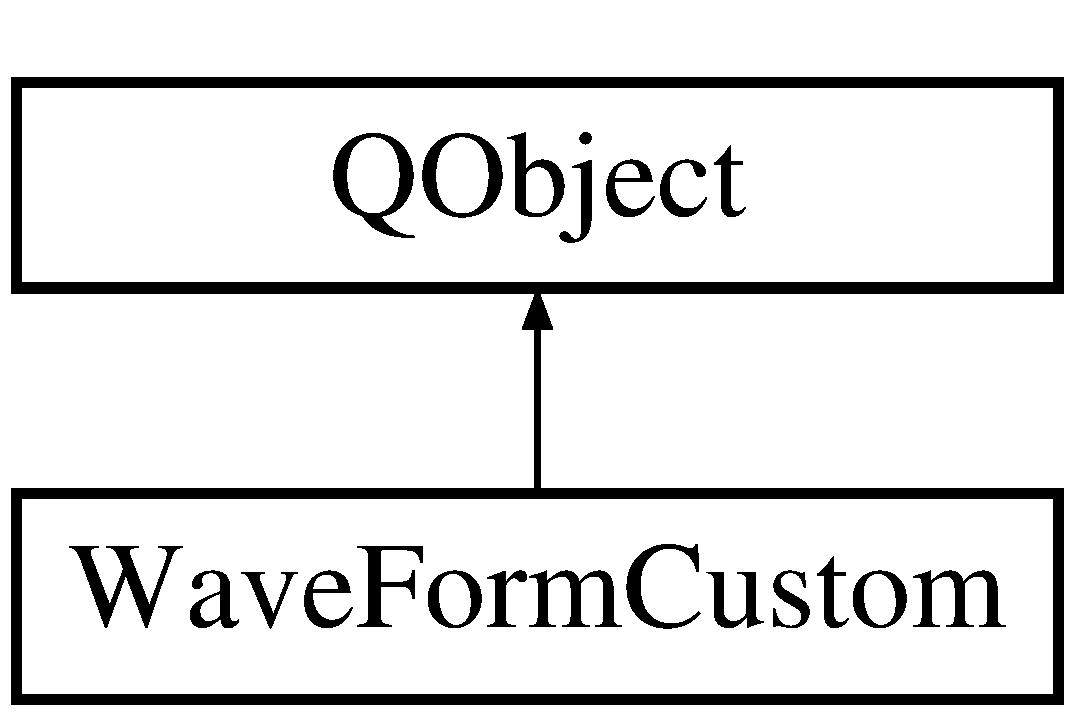
\includegraphics[height=2.000000cm]{class_wave_form_custom}
\end{center}
\end{figure}
\subsection*{Public Slots}
\begin{DoxyCompactItemize}
\item 
void \hyperlink{class_wave_form_custom_ab69bdeeb043d9304d19723e4b35c2f33}{generate\+Data} (int type, int row\+Count, int col\+Count)
\item 
void \hyperlink{class_wave_form_custom_a78ba2270b3d08781fac5de6b39cb3a53}{buffer\+Changed} (qint64 position, qint64 length, const Q\+Byte\+Array \&\hyperlink{class_wave_form_custom_a90fb1825e9929177cf5e034a464e4e24}{buffer})
\item 
Q\+Abstract\+Series $\ast$ \hyperlink{class_wave_form_custom_a76683067d578c13b6f5141c74590a746}{get\+Series} () const
\item 
void \hyperlink{class_wave_form_custom_ac6c2dbc11bd5789cee99674077307799}{subscribe\+Series} (Q\+Abstract\+Series $\ast$value, int channel\+Count)
\item 
bool \hyperlink{class_wave_form_custom_a51bbb3f0a646f2fbac70617cad686d75}{un\+Subscribe\+Series} (Q\+Abstract\+Series $\ast$value, int channel\+Count)
\end{DoxyCompactItemize}
\subsection*{Public Member Functions}
\begin{DoxyCompactItemize}
\item 
\hyperlink{class_wave_form_custom_af4c78a9a88ccb502909249d5069bb238}{Wave\+Form\+Custom} (Q\+Object $\ast$parent=0)
\item 
Q\+Audio\+Format \hyperlink{class_wave_form_custom_a4fc6efc93c4e13d29fb5cbabb8354cfb}{format} () const
\item 
void \hyperlink{class_wave_form_custom_a4280e281f1b4e91710c791751b4c956d}{set\+Format} (const Q\+Audio\+Format \&\hyperlink{class_wave_form_custom_a4fc6efc93c4e13d29fb5cbabb8354cfb}{format})
\item 
Q\+Byte\+Array \hyperlink{class_wave_form_custom_a90fb1825e9929177cf5e034a464e4e24}{buffer} () const
\item 
void \hyperlink{class_wave_form_custom_aa30d2651a92723178f74d0d14fa13809}{set\+Buffer} (const Q\+Byte\+Array \&\hyperlink{class_wave_form_custom_a90fb1825e9929177cf5e034a464e4e24}{buffer})
\end{DoxyCompactItemize}


\subsection{Constructor \& Destructor Documentation}
\hypertarget{class_wave_form_custom_af4c78a9a88ccb502909249d5069bb238}{}\label{class_wave_form_custom_af4c78a9a88ccb502909249d5069bb238} 
\index{Wave\+Form\+Custom@{Wave\+Form\+Custom}!Wave\+Form\+Custom@{Wave\+Form\+Custom}}
\index{Wave\+Form\+Custom@{Wave\+Form\+Custom}!Wave\+Form\+Custom@{Wave\+Form\+Custom}}
\subsubsection{\texorpdfstring{Wave\+Form\+Custom()}{WaveFormCustom()}}
{\footnotesize\ttfamily Q\+T\+\_\+\+C\+H\+A\+R\+T\+S\+\_\+\+U\+S\+E\+\_\+\+N\+A\+M\+E\+S\+P\+A\+CE Wave\+Form\+Custom\+::\+Wave\+Form\+Custom (\begin{DoxyParamCaption}\item[{Q\+Object $\ast$}]{parent = {\ttfamily 0} }\end{DoxyParamCaption})\hspace{0.3cm}{\ttfamily [explicit]}}



\subsection{Member Function Documentation}
\hypertarget{class_wave_form_custom_a90fb1825e9929177cf5e034a464e4e24}{}\label{class_wave_form_custom_a90fb1825e9929177cf5e034a464e4e24} 
\index{Wave\+Form\+Custom@{Wave\+Form\+Custom}!buffer@{buffer}}
\index{buffer@{buffer}!Wave\+Form\+Custom@{Wave\+Form\+Custom}}
\subsubsection{\texorpdfstring{buffer()}{buffer()}}
{\footnotesize\ttfamily Q\+Byte\+Array Wave\+Form\+Custom\+::buffer (\begin{DoxyParamCaption}{ }\end{DoxyParamCaption}) const}

\hypertarget{class_wave_form_custom_a78ba2270b3d08781fac5de6b39cb3a53}{}\label{class_wave_form_custom_a78ba2270b3d08781fac5de6b39cb3a53} 
\index{Wave\+Form\+Custom@{Wave\+Form\+Custom}!buffer\+Changed@{buffer\+Changed}}
\index{buffer\+Changed@{buffer\+Changed}!Wave\+Form\+Custom@{Wave\+Form\+Custom}}
\subsubsection{\texorpdfstring{buffer\+Changed}{bufferChanged}}
{\footnotesize\ttfamily void Wave\+Form\+Custom\+::buffer\+Changed (\begin{DoxyParamCaption}\item[{qint64}]{position,  }\item[{qint64}]{length,  }\item[{const Q\+Byte\+Array \&}]{buffer }\end{DoxyParamCaption})\hspace{0.3cm}{\ttfamily [slot]}}

\hypertarget{class_wave_form_custom_a4fc6efc93c4e13d29fb5cbabb8354cfb}{}\label{class_wave_form_custom_a4fc6efc93c4e13d29fb5cbabb8354cfb} 
\index{Wave\+Form\+Custom@{Wave\+Form\+Custom}!format@{format}}
\index{format@{format}!Wave\+Form\+Custom@{Wave\+Form\+Custom}}
\subsubsection{\texorpdfstring{format()}{format()}}
{\footnotesize\ttfamily Q\+Audio\+Format Wave\+Form\+Custom\+::format (\begin{DoxyParamCaption}{ }\end{DoxyParamCaption}) const}

\hypertarget{class_wave_form_custom_ab69bdeeb043d9304d19723e4b35c2f33}{}\label{class_wave_form_custom_ab69bdeeb043d9304d19723e4b35c2f33} 
\index{Wave\+Form\+Custom@{Wave\+Form\+Custom}!generate\+Data@{generate\+Data}}
\index{generate\+Data@{generate\+Data}!Wave\+Form\+Custom@{Wave\+Form\+Custom}}
\subsubsection{\texorpdfstring{generate\+Data}{generateData}}
{\footnotesize\ttfamily void Wave\+Form\+Custom\+::generate\+Data (\begin{DoxyParamCaption}\item[{int}]{type,  }\item[{int}]{row\+Count,  }\item[{int}]{col\+Count }\end{DoxyParamCaption})\hspace{0.3cm}{\ttfamily [slot]}}

\hypertarget{class_wave_form_custom_a76683067d578c13b6f5141c74590a746}{}\label{class_wave_form_custom_a76683067d578c13b6f5141c74590a746} 
\index{Wave\+Form\+Custom@{Wave\+Form\+Custom}!get\+Series@{get\+Series}}
\index{get\+Series@{get\+Series}!Wave\+Form\+Custom@{Wave\+Form\+Custom}}
\subsubsection{\texorpdfstring{get\+Series}{getSeries}}
{\footnotesize\ttfamily Q\+Abstract\+Series $\ast$ Wave\+Form\+Custom\+::get\+Series (\begin{DoxyParamCaption}{ }\end{DoxyParamCaption}) const\hspace{0.3cm}{\ttfamily [slot]}}

\hypertarget{class_wave_form_custom_aa30d2651a92723178f74d0d14fa13809}{}\label{class_wave_form_custom_aa30d2651a92723178f74d0d14fa13809} 
\index{Wave\+Form\+Custom@{Wave\+Form\+Custom}!set\+Buffer@{set\+Buffer}}
\index{set\+Buffer@{set\+Buffer}!Wave\+Form\+Custom@{Wave\+Form\+Custom}}
\subsubsection{\texorpdfstring{set\+Buffer()}{setBuffer()}}
{\footnotesize\ttfamily void Wave\+Form\+Custom\+::set\+Buffer (\begin{DoxyParamCaption}\item[{const Q\+Byte\+Array \&}]{buffer }\end{DoxyParamCaption})}

\hypertarget{class_wave_form_custom_a4280e281f1b4e91710c791751b4c956d}{}\label{class_wave_form_custom_a4280e281f1b4e91710c791751b4c956d} 
\index{Wave\+Form\+Custom@{Wave\+Form\+Custom}!set\+Format@{set\+Format}}
\index{set\+Format@{set\+Format}!Wave\+Form\+Custom@{Wave\+Form\+Custom}}
\subsubsection{\texorpdfstring{set\+Format()}{setFormat()}}
{\footnotesize\ttfamily void Wave\+Form\+Custom\+::set\+Format (\begin{DoxyParamCaption}\item[{const Q\+Audio\+Format \&}]{format }\end{DoxyParamCaption})}

\hypertarget{class_wave_form_custom_ac6c2dbc11bd5789cee99674077307799}{}\label{class_wave_form_custom_ac6c2dbc11bd5789cee99674077307799} 
\index{Wave\+Form\+Custom@{Wave\+Form\+Custom}!subscribe\+Series@{subscribe\+Series}}
\index{subscribe\+Series@{subscribe\+Series}!Wave\+Form\+Custom@{Wave\+Form\+Custom}}
\subsubsection{\texorpdfstring{subscribe\+Series}{subscribeSeries}}
{\footnotesize\ttfamily void Wave\+Form\+Custom\+::subscribe\+Series (\begin{DoxyParamCaption}\item[{Q\+Abstract\+Series $\ast$}]{value,  }\item[{int}]{channel\+Count }\end{DoxyParamCaption})\hspace{0.3cm}{\ttfamily [slot]}}

\hypertarget{class_wave_form_custom_a51bbb3f0a646f2fbac70617cad686d75}{}\label{class_wave_form_custom_a51bbb3f0a646f2fbac70617cad686d75} 
\index{Wave\+Form\+Custom@{Wave\+Form\+Custom}!un\+Subscribe\+Series@{un\+Subscribe\+Series}}
\index{un\+Subscribe\+Series@{un\+Subscribe\+Series}!Wave\+Form\+Custom@{Wave\+Form\+Custom}}
\subsubsection{\texorpdfstring{un\+Subscribe\+Series}{unSubscribeSeries}}
{\footnotesize\ttfamily bool Wave\+Form\+Custom\+::un\+Subscribe\+Series (\begin{DoxyParamCaption}\item[{Q\+Abstract\+Series $\ast$}]{value,  }\item[{int}]{channel\+Count }\end{DoxyParamCaption})\hspace{0.3cm}{\ttfamily [slot]}}



The documentation for this class was generated from the following files\+:\begin{DoxyCompactItemize}
\item 
app/\hyperlink{datasource_8h}{datasource.\+h}\item 
app/\hyperlink{datasource_8cpp}{datasource.\+cpp}\end{DoxyCompactItemize}

\hypertarget{struct_w_a_v_e_header}{}\section{W\+A\+V\+E\+Header Struct Reference}
\label{struct_w_a_v_e_header}\index{W\+A\+V\+E\+Header@{W\+A\+V\+E\+Header}}
\subsection*{Public Attributes}
\begin{DoxyCompactItemize}
\item 
\hyperlink{structchunk}{chunk} \hyperlink{struct_w_a_v_e_header_a763f44cebee2065d899d5997e9b22e60}{descriptor}
\item 
quint16 \hyperlink{struct_w_a_v_e_header_adaa2b3225220ab7448035e656c6669d9}{audio\+Format}
\item 
quint16 \hyperlink{struct_w_a_v_e_header_a547399f45cc973c818b62fe5410cdd04}{num\+Channels}
\item 
quint32 \hyperlink{struct_w_a_v_e_header_aa4f1b67d3e8e2d455f4f5fbc61c82c2d}{sample\+Rate}
\item 
quint32 \hyperlink{struct_w_a_v_e_header_aa0db8c5f2933a00865fabab8d1faa014}{byte\+Rate}
\item 
quint16 \hyperlink{struct_w_a_v_e_header_a9c53314461e82fa197f69dd44ba1eacc}{block\+Align}
\item 
quint16 \hyperlink{struct_w_a_v_e_header_a0847636e0f72678c584b1506e569e19d}{bits\+Per\+Sample}
\end{DoxyCompactItemize}


\subsection{Member Data Documentation}
\hypertarget{struct_w_a_v_e_header_adaa2b3225220ab7448035e656c6669d9}{}\label{struct_w_a_v_e_header_adaa2b3225220ab7448035e656c6669d9} 
\index{W\+A\+V\+E\+Header@{W\+A\+V\+E\+Header}!audio\+Format@{audio\+Format}}
\index{audio\+Format@{audio\+Format}!W\+A\+V\+E\+Header@{W\+A\+V\+E\+Header}}
\subsubsection{\texorpdfstring{audio\+Format}{audioFormat}}
{\footnotesize\ttfamily quint16 W\+A\+V\+E\+Header\+::audio\+Format}

\hypertarget{struct_w_a_v_e_header_a0847636e0f72678c584b1506e569e19d}{}\label{struct_w_a_v_e_header_a0847636e0f72678c584b1506e569e19d} 
\index{W\+A\+V\+E\+Header@{W\+A\+V\+E\+Header}!bits\+Per\+Sample@{bits\+Per\+Sample}}
\index{bits\+Per\+Sample@{bits\+Per\+Sample}!W\+A\+V\+E\+Header@{W\+A\+V\+E\+Header}}
\subsubsection{\texorpdfstring{bits\+Per\+Sample}{bitsPerSample}}
{\footnotesize\ttfamily quint16 W\+A\+V\+E\+Header\+::bits\+Per\+Sample}

\hypertarget{struct_w_a_v_e_header_a9c53314461e82fa197f69dd44ba1eacc}{}\label{struct_w_a_v_e_header_a9c53314461e82fa197f69dd44ba1eacc} 
\index{W\+A\+V\+E\+Header@{W\+A\+V\+E\+Header}!block\+Align@{block\+Align}}
\index{block\+Align@{block\+Align}!W\+A\+V\+E\+Header@{W\+A\+V\+E\+Header}}
\subsubsection{\texorpdfstring{block\+Align}{blockAlign}}
{\footnotesize\ttfamily quint16 W\+A\+V\+E\+Header\+::block\+Align}

\hypertarget{struct_w_a_v_e_header_aa0db8c5f2933a00865fabab8d1faa014}{}\label{struct_w_a_v_e_header_aa0db8c5f2933a00865fabab8d1faa014} 
\index{W\+A\+V\+E\+Header@{W\+A\+V\+E\+Header}!byte\+Rate@{byte\+Rate}}
\index{byte\+Rate@{byte\+Rate}!W\+A\+V\+E\+Header@{W\+A\+V\+E\+Header}}
\subsubsection{\texorpdfstring{byte\+Rate}{byteRate}}
{\footnotesize\ttfamily quint32 W\+A\+V\+E\+Header\+::byte\+Rate}

\hypertarget{struct_w_a_v_e_header_a763f44cebee2065d899d5997e9b22e60}{}\label{struct_w_a_v_e_header_a763f44cebee2065d899d5997e9b22e60} 
\index{W\+A\+V\+E\+Header@{W\+A\+V\+E\+Header}!descriptor@{descriptor}}
\index{descriptor@{descriptor}!W\+A\+V\+E\+Header@{W\+A\+V\+E\+Header}}
\subsubsection{\texorpdfstring{descriptor}{descriptor}}
{\footnotesize\ttfamily \hyperlink{structchunk}{chunk} W\+A\+V\+E\+Header\+::descriptor}

\hypertarget{struct_w_a_v_e_header_a547399f45cc973c818b62fe5410cdd04}{}\label{struct_w_a_v_e_header_a547399f45cc973c818b62fe5410cdd04} 
\index{W\+A\+V\+E\+Header@{W\+A\+V\+E\+Header}!num\+Channels@{num\+Channels}}
\index{num\+Channels@{num\+Channels}!W\+A\+V\+E\+Header@{W\+A\+V\+E\+Header}}
\subsubsection{\texorpdfstring{num\+Channels}{numChannels}}
{\footnotesize\ttfamily quint16 W\+A\+V\+E\+Header\+::num\+Channels}

\hypertarget{struct_w_a_v_e_header_aa4f1b67d3e8e2d455f4f5fbc61c82c2d}{}\label{struct_w_a_v_e_header_aa4f1b67d3e8e2d455f4f5fbc61c82c2d} 
\index{W\+A\+V\+E\+Header@{W\+A\+V\+E\+Header}!sample\+Rate@{sample\+Rate}}
\index{sample\+Rate@{sample\+Rate}!W\+A\+V\+E\+Header@{W\+A\+V\+E\+Header}}
\subsubsection{\texorpdfstring{sample\+Rate}{sampleRate}}
{\footnotesize\ttfamily quint32 W\+A\+V\+E\+Header\+::sample\+Rate}



The documentation for this struct was generated from the following file\+:\begin{DoxyCompactItemize}
\item 
app/\hyperlink{wavfile_8cpp}{wavfile.\+cpp}\end{DoxyCompactItemize}

\hypertarget{class_wav_file}{}\section{Wav\+File Class Reference}
\label{class_wav_file}\index{Wav\+File@{Wav\+File}}


The \hyperlink{class_wav_file}{Wav\+File} class Simple wraper to wav file.  




{\ttfamily \#include $<$wavfile.\+h$>$}

Inheritance diagram for Wav\+File\+:\begin{figure}[H]
\begin{center}
\leavevmode
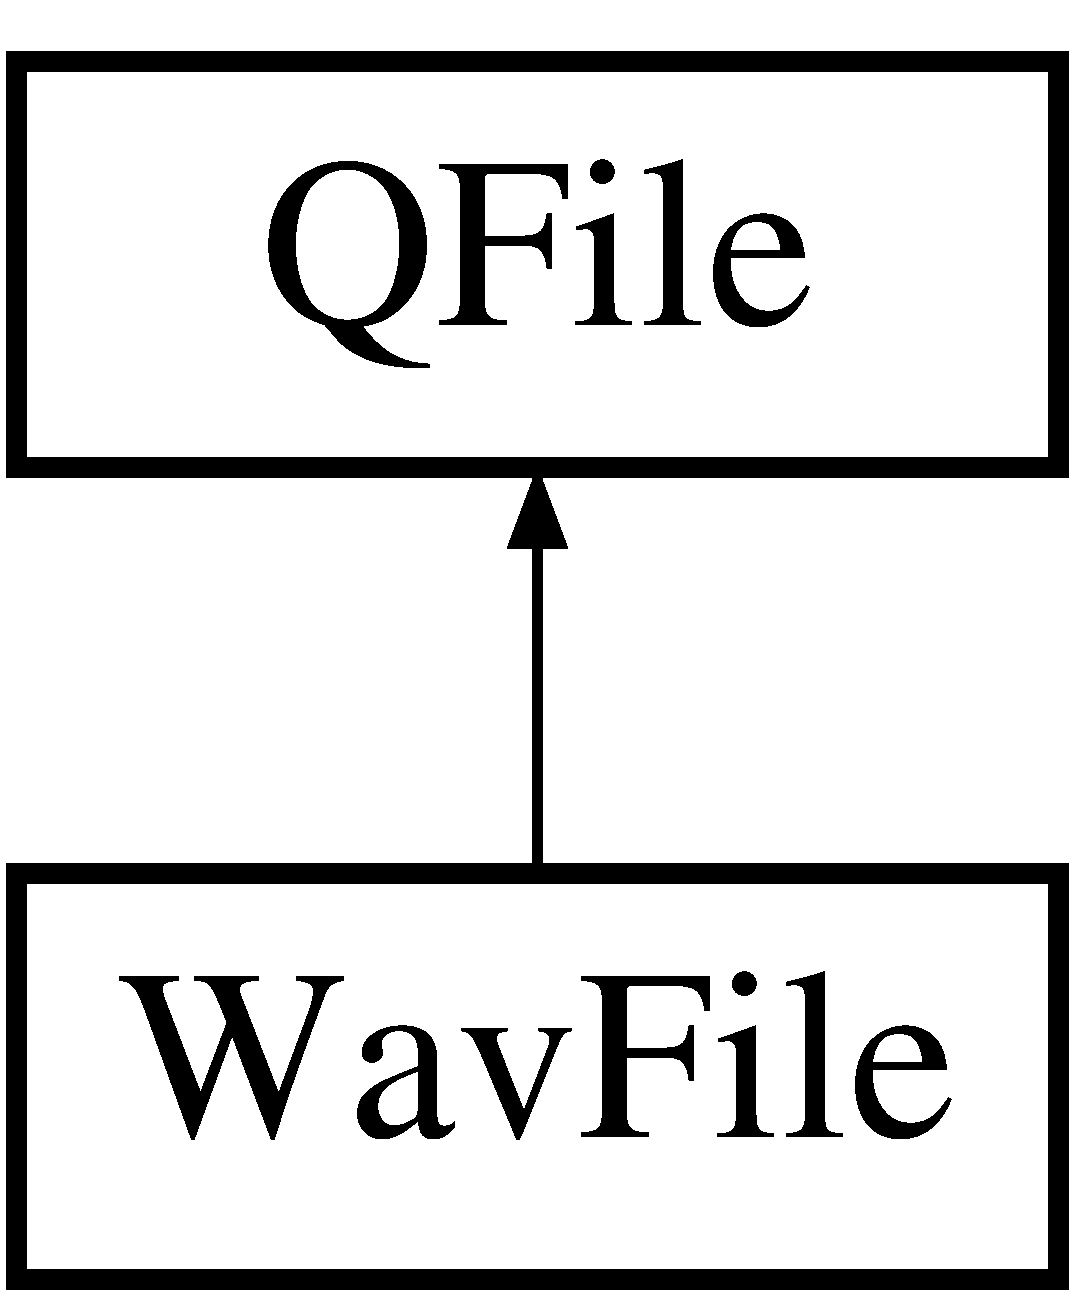
\includegraphics[height=2.000000cm]{class_wav_file}
\end{center}
\end{figure}
\subsection*{Public Member Functions}
\begin{DoxyCompactItemize}
\item 
\hyperlink{class_wav_file_afaaa4dfab63fc0f4554ee36184c7b3d4}{Wav\+File} (Q\+Object $\ast$parent=0)
\item 
bool \hyperlink{class_wav_file_a60680d00e08ed8ebbe33d624b6d0cd16}{open} (const Q\+String \&file\+Name)
\item 
const Q\+Audio\+Format \& \hyperlink{class_wav_file_a9b2f3e3e7602540cda66562db243e332}{file\+Format} () const
\item 
qint64 \hyperlink{class_wav_file_a800a698411cfd6f5fdecc42beb053fb9}{header\+Length} () const
\end{DoxyCompactItemize}


\subsection{Detailed Description}
The \hyperlink{class_wav_file}{Wav\+File} class Simple wraper to wav file. 

\subsection{Constructor \& Destructor Documentation}
\hypertarget{class_wav_file_afaaa4dfab63fc0f4554ee36184c7b3d4}{}\label{class_wav_file_afaaa4dfab63fc0f4554ee36184c7b3d4} 
\index{Wav\+File@{Wav\+File}!Wav\+File@{Wav\+File}}
\index{Wav\+File@{Wav\+File}!Wav\+File@{Wav\+File}}
\subsubsection{\texorpdfstring{Wav\+File()}{WavFile()}}
{\footnotesize\ttfamily Wav\+File\+::\+Wav\+File (\begin{DoxyParamCaption}\item[{Q\+Object $\ast$}]{parent = {\ttfamily 0} }\end{DoxyParamCaption})}



\subsection{Member Function Documentation}
\hypertarget{class_wav_file_a9b2f3e3e7602540cda66562db243e332}{}\label{class_wav_file_a9b2f3e3e7602540cda66562db243e332} 
\index{Wav\+File@{Wav\+File}!file\+Format@{file\+Format}}
\index{file\+Format@{file\+Format}!Wav\+File@{Wav\+File}}
\subsubsection{\texorpdfstring{file\+Format()}{fileFormat()}}
{\footnotesize\ttfamily const Q\+Audio\+Format \& Wav\+File\+::file\+Format (\begin{DoxyParamCaption}{ }\end{DoxyParamCaption}) const}

\hypertarget{class_wav_file_a800a698411cfd6f5fdecc42beb053fb9}{}\label{class_wav_file_a800a698411cfd6f5fdecc42beb053fb9} 
\index{Wav\+File@{Wav\+File}!header\+Length@{header\+Length}}
\index{header\+Length@{header\+Length}!Wav\+File@{Wav\+File}}
\subsubsection{\texorpdfstring{header\+Length()}{headerLength()}}
{\footnotesize\ttfamily qint64 Wav\+File\+::header\+Length (\begin{DoxyParamCaption}{ }\end{DoxyParamCaption}) const}

\hypertarget{class_wav_file_a60680d00e08ed8ebbe33d624b6d0cd16}{}\label{class_wav_file_a60680d00e08ed8ebbe33d624b6d0cd16} 
\index{Wav\+File@{Wav\+File}!open@{open}}
\index{open@{open}!Wav\+File@{Wav\+File}}
\subsubsection{\texorpdfstring{open()}{open()}}
{\footnotesize\ttfamily bool Wav\+File\+::open (\begin{DoxyParamCaption}\item[{const Q\+String \&}]{file\+Name }\end{DoxyParamCaption})}



The documentation for this class was generated from the following files\+:\begin{DoxyCompactItemize}
\item 
app/\hyperlink{wavfile_8h}{wavfile.\+h}\item 
app/\hyperlink{wavfile_8cpp}{wavfile.\+cpp}\end{DoxyCompactItemize}

\chapter{File Documentation}
\hypertarget{customfilter_8cpp}{}\section{app/customfilter.cpp File Reference}
\label{customfilter_8cpp}\index{app/customfilter.\+cpp@{app/customfilter.\+cpp}}
{\ttfamily \#include \char`\"{}customfilter.\+h\char`\"{}}\newline
\subsection*{Macros}
\begin{DoxyCompactItemize}
\item 
\#define \hyperlink{customfilter_8cpp_ac53f25ffb384c817aa47772fff2ee63e}{G\+E\+T\+M\+A\+SK}(index,  size)~(((1 $<$$<$ (size)) -\/ 1) $<$$<$ (index))
\item 
\#define \hyperlink{customfilter_8cpp_a313c096e8acd01970ca4b732f6feb099}{R\+E\+A\+D\+F\+R\+OM}(data,  index,  size)~(((data) \& \hyperlink{customfilter_8cpp_ac53f25ffb384c817aa47772fff2ee63e}{G\+E\+T\+M\+A\+SK}((index), (size))) $>$$>$ (index))
\item 
\#define \hyperlink{customfilter_8cpp_af1e7ae2afb5fba6fe89bf838b009704e}{W\+R\+I\+T\+E\+TO}(data,  index,  size,  value)~((data) = ((data) \& ($\sim$\hyperlink{customfilter_8cpp_ac53f25ffb384c817aa47772fff2ee63e}{G\+E\+T\+M\+A\+SK}((index), (size)))) $\vert$ ((value) $<$$<$ (index)))
\end{DoxyCompactItemize}


\subsection{Macro Definition Documentation}
\hypertarget{customfilter_8cpp_ac53f25ffb384c817aa47772fff2ee63e}{}\label{customfilter_8cpp_ac53f25ffb384c817aa47772fff2ee63e} 
\index{customfilter.\+cpp@{customfilter.\+cpp}!G\+E\+T\+M\+A\+SK@{G\+E\+T\+M\+A\+SK}}
\index{G\+E\+T\+M\+A\+SK@{G\+E\+T\+M\+A\+SK}!customfilter.\+cpp@{customfilter.\+cpp}}
\subsubsection{\texorpdfstring{G\+E\+T\+M\+A\+SK}{GETMASK}}
{\footnotesize\ttfamily \#define G\+E\+T\+M\+A\+SK(\begin{DoxyParamCaption}\item[{}]{index,  }\item[{}]{size }\end{DoxyParamCaption})~(((1 $<$$<$ (size)) -\/ 1) $<$$<$ (index))}

\hypertarget{customfilter_8cpp_a313c096e8acd01970ca4b732f6feb099}{}\label{customfilter_8cpp_a313c096e8acd01970ca4b732f6feb099} 
\index{customfilter.\+cpp@{customfilter.\+cpp}!R\+E\+A\+D\+F\+R\+OM@{R\+E\+A\+D\+F\+R\+OM}}
\index{R\+E\+A\+D\+F\+R\+OM@{R\+E\+A\+D\+F\+R\+OM}!customfilter.\+cpp@{customfilter.\+cpp}}
\subsubsection{\texorpdfstring{R\+E\+A\+D\+F\+R\+OM}{READFROM}}
{\footnotesize\ttfamily \#define R\+E\+A\+D\+F\+R\+OM(\begin{DoxyParamCaption}\item[{}]{data,  }\item[{}]{index,  }\item[{}]{size }\end{DoxyParamCaption})~(((data) \& \hyperlink{customfilter_8cpp_ac53f25ffb384c817aa47772fff2ee63e}{G\+E\+T\+M\+A\+SK}((index), (size))) $>$$>$ (index))}

\hypertarget{customfilter_8cpp_af1e7ae2afb5fba6fe89bf838b009704e}{}\label{customfilter_8cpp_af1e7ae2afb5fba6fe89bf838b009704e} 
\index{customfilter.\+cpp@{customfilter.\+cpp}!W\+R\+I\+T\+E\+TO@{W\+R\+I\+T\+E\+TO}}
\index{W\+R\+I\+T\+E\+TO@{W\+R\+I\+T\+E\+TO}!customfilter.\+cpp@{customfilter.\+cpp}}
\subsubsection{\texorpdfstring{W\+R\+I\+T\+E\+TO}{WRITETO}}
{\footnotesize\ttfamily \#define W\+R\+I\+T\+E\+TO(\begin{DoxyParamCaption}\item[{}]{data,  }\item[{}]{index,  }\item[{}]{size,  }\item[{}]{value }\end{DoxyParamCaption})~((data) = ((data) \& ($\sim$\hyperlink{customfilter_8cpp_ac53f25ffb384c817aa47772fff2ee63e}{G\+E\+T\+M\+A\+SK}((index), (size)))) $\vert$ ((value) $<$$<$ (index)))}


\hypertarget{customfilter_8h}{}\section{app/customfilter.h File Reference}
\label{customfilter_8h}\index{app/customfilter.\+h@{app/customfilter.\+h}}
{\ttfamily \#include $<$Q\+Object$>$}\newline
{\ttfamily \#include \char`\"{}filter.\+h\char`\"{}}\newline
{\ttfamily \#include $<$Q\+Audio\+Format$>$}\newline
{\ttfamily \#include $<$Q\+Debug$>$}\newline
{\ttfamily \#include $<$Qt\+Core$>$}\newline
\subsection*{Classes}
\begin{DoxyCompactItemize}
\item 
class \hyperlink{class_custom_filter}{Custom\+Filter}
\begin{DoxyCompactList}\small\item\em Simple filter type. which can use an array of input dividers for filtering. \end{DoxyCompactList}\end{DoxyCompactItemize}

\hypertarget{datasource_8cpp}{}\section{app/datasource.cpp File Reference}
\label{datasource_8cpp}\index{app/datasource.\+cpp@{app/datasource.\+cpp}}
{\ttfamily \#include \char`\"{}datasource.\+h\char`\"{}}\newline
{\ttfamily \#include $<$Qt\+Charts/\+Q\+X\+Y\+Series$>$}\newline
{\ttfamily \#include $<$Qt\+Charts/\+Q\+Area\+Series$>$}\newline
{\ttfamily \#include $<$Qt\+Quick/\+Q\+Quick\+View$>$}\newline
{\ttfamily \#include $<$Qt\+Quick/\+Q\+Quick\+Item$>$}\newline
{\ttfamily \#include $<$Qt\+Core/\+Q\+Debug$>$}\newline
{\ttfamily \#include $<$Qt\+Core/\+Qt\+Math$>$}\newline

\hypertarget{datasource_8h}{}\section{app/datasource.h File Reference}
\label{datasource_8h}\index{app/datasource.\+h@{app/datasource.\+h}}
{\ttfamily \#include $<$Qt\+Core/\+Q\+Object$>$}\newline
{\ttfamily \#include $<$Qt\+Charts/\+Q\+Abstract\+Series$>$}\newline
{\ttfamily \#include $<$Q\+Audio\+Format$>$}\newline
\subsection*{Classes}
\begin{DoxyCompactItemize}
\item 
struct \hyperlink{struct_series_chanel}{Series\+Chanel}
\item 
class \hyperlink{class_wave_form_custom}{Wave\+Form\+Custom}
\end{DoxyCompactItemize}

\hypertarget{engine_8cpp}{}\section{app/engine.cpp File Reference}
\label{engine_8cpp}\index{app/engine.\+cpp@{app/engine.\+cpp}}
{\ttfamily \#include \char`\"{}engine.\+h\char`\"{}}\newline
{\ttfamily \#include \char`\"{}utils.\+h\char`\"{}}\newline
{\ttfamily \#include $<$math.\+h$>$}\newline
{\ttfamily \#include $<$Q\+Audio\+Input$>$}\newline
{\ttfamily \#include $<$Q\+Audio\+Output$>$}\newline
{\ttfamily \#include $<$Q\+Core\+Application$>$}\newline
{\ttfamily \#include $<$Q\+Debug$>$}\newline
{\ttfamily \#include $<$Q\+File$>$}\newline
{\ttfamily \#include $<$Q\+Meta\+Object$>$}\newline
{\ttfamily \#include $<$Q\+Set$>$}\newline
{\ttfamily \#include $<$Q\+Thread$>$}\newline
\subsection*{Variables}
\begin{DoxyCompactItemize}
\item 
const qint64 \hyperlink{engine_8cpp_a00a87b0fed28519f6b1894976f53e1c0}{Buffer\+Duration\+Us} = 100 $\ast$ 1000000
\item 
const int \hyperlink{engine_8cpp_ae21024152235cc77873acbaccaf0de55}{Notify\+Interval\+Ms} = 1
\item 
const int \hyperlink{engine_8cpp_ac44d91f7aca6b4b5ce2a616902bb6db3}{Level\+Window\+Us} = 0.\+1 $\ast$ 1000000
\end{DoxyCompactItemize}


\subsection{Variable Documentation}
\hypertarget{engine_8cpp_a00a87b0fed28519f6b1894976f53e1c0}{}\label{engine_8cpp_a00a87b0fed28519f6b1894976f53e1c0} 
\index{engine.\+cpp@{engine.\+cpp}!Buffer\+Duration\+Us@{Buffer\+Duration\+Us}}
\index{Buffer\+Duration\+Us@{Buffer\+Duration\+Us}!engine.\+cpp@{engine.\+cpp}}
\subsubsection{\texorpdfstring{Buffer\+Duration\+Us}{BufferDurationUs}}
{\footnotesize\ttfamily const qint64 Buffer\+Duration\+Us = 100 $\ast$ 1000000}

\hypertarget{engine_8cpp_ac44d91f7aca6b4b5ce2a616902bb6db3}{}\label{engine_8cpp_ac44d91f7aca6b4b5ce2a616902bb6db3} 
\index{engine.\+cpp@{engine.\+cpp}!Level\+Window\+Us@{Level\+Window\+Us}}
\index{Level\+Window\+Us@{Level\+Window\+Us}!engine.\+cpp@{engine.\+cpp}}
\subsubsection{\texorpdfstring{Level\+Window\+Us}{LevelWindowUs}}
{\footnotesize\ttfamily const int Level\+Window\+Us = 0.\+1 $\ast$ 1000000}

\hypertarget{engine_8cpp_ae21024152235cc77873acbaccaf0de55}{}\label{engine_8cpp_ae21024152235cc77873acbaccaf0de55} 
\index{engine.\+cpp@{engine.\+cpp}!Notify\+Interval\+Ms@{Notify\+Interval\+Ms}}
\index{Notify\+Interval\+Ms@{Notify\+Interval\+Ms}!engine.\+cpp@{engine.\+cpp}}
\subsubsection{\texorpdfstring{Notify\+Interval\+Ms}{NotifyIntervalMs}}
{\footnotesize\ttfamily const int Notify\+Interval\+Ms = 1}


\hypertarget{engine_8h}{}\section{app/engine.h File Reference}
\label{engine_8h}\index{app/engine.\+h@{app/engine.\+h}}
{\ttfamily \#include \char`\"{}graphfilterservice.\+h\char`\"{}}\newline
{\ttfamily \#include \char`\"{}spectrum.\+h\char`\"{}}\newline
{\ttfamily \#include \char`\"{}spectrumanalyser.\+h\char`\"{}}\newline
{\ttfamily \#include \char`\"{}wavfile.\+h\char`\"{}}\newline
{\ttfamily \#include \char`\"{}nullfilter.\+h\char`\"{}}\newline
{\ttfamily \#include \char`\"{}customfilter.\+h\char`\"{}}\newline
{\ttfamily \#include $<$Q\+Audio\+Device\+Info$>$}\newline
{\ttfamily \#include $<$Q\+Audio\+Format$>$}\newline
{\ttfamily \#include $<$Q\+Buffer$>$}\newline
{\ttfamily \#include $<$Q\+Byte\+Array$>$}\newline
{\ttfamily \#include $<$Q\+Dir$>$}\newline
{\ttfamily \#include $<$Q\+Object$>$}\newline
{\ttfamily \#include $<$Q\+Vector$>$}\newline
{\ttfamily \#include $<$Q\+Timer$>$}\newline
\subsection*{Classes}
\begin{DoxyCompactItemize}
\item 
class \hyperlink{class_engine}{Engine}
\end{DoxyCompactItemize}

\hypertarget{filter_8cpp}{}\section{app/filter.cpp File Reference}
\label{filter_8cpp}\index{app/filter.\+cpp@{app/filter.\+cpp}}
{\ttfamily \#include \char`\"{}filter.\+h\char`\"{}}\newline

\hypertarget{filter_8h}{}\section{app/filter.h File Reference}
\label{filter_8h}\index{app/filter.\+h@{app/filter.\+h}}
{\ttfamily \#include $<$Q\+Object$>$}\newline
{\ttfamily \#include $<$Q\+Audio\+Format$>$}\newline
\subsection*{Classes}
\begin{DoxyCompactItemize}
\item 
class \hyperlink{class_filter}{Filter}
\begin{DoxyCompactList}\small\item\em The \hyperlink{class_filter}{Filter} class  abstract vision of filter. \end{DoxyCompactList}\end{DoxyCompactItemize}

\hypertarget{frequencyspectrum_8cpp}{}\section{app/frequencyspectrum.cpp File Reference}
\label{frequencyspectrum_8cpp}\index{app/frequencyspectrum.\+cpp@{app/frequencyspectrum.\+cpp}}
{\ttfamily \#include \char`\"{}frequencyspectrum.\+h\char`\"{}}\newline

\hypertarget{frequencyspectrum_8h}{}\section{app/frequencyspectrum.h File Reference}
\label{frequencyspectrum_8h}\index{app/frequencyspectrum.\+h@{app/frequencyspectrum.\+h}}
{\ttfamily \#include $<$Qt\+Core/\+Q\+Vector$>$}\newline
\subsection*{Classes}
\begin{DoxyCompactItemize}
\item 
class \hyperlink{class_frequency_spectrum}{Frequency\+Spectrum}
\item 
struct \hyperlink{struct_frequency_spectrum_1_1_element}{Frequency\+Spectrum\+::\+Element}
\end{DoxyCompactItemize}

\hypertarget{graph_8cpp}{}\section{app/graph.cpp File Reference}
\label{graph_8cpp}\index{app/graph.\+cpp@{app/graph.\+cpp}}
{\ttfamily \#include \char`\"{}graph.\+h\char`\"{}}\newline

\hypertarget{graph_8h}{}\section{app/graph.h File Reference}
\label{graph_8h}\index{app/graph.\+h@{app/graph.\+h}}
{\ttfamily \#include $<$Q\+Object$>$}\newline
\subsection*{Classes}
\begin{DoxyCompactItemize}
\item 
class \hyperlink{class_graph}{Graph}
\end{DoxyCompactItemize}

\hypertarget{graphfilterservice_8cpp}{}\section{app/graphfilterservice.cpp File Reference}
\label{graphfilterservice_8cpp}\index{app/graphfilterservice.\+cpp@{app/graphfilterservice.\+cpp}}
{\ttfamily \#include \char`\"{}graphfilterservice.\+h\char`\"{}}\newline
{\ttfamily \#include \char`\"{}engine.\+h\char`\"{}}\newline

\hypertarget{graphfilterservice_8h}{}\section{app/graphfilterservice.h File Reference}
\label{graphfilterservice_8h}\index{app/graphfilterservice.\+h@{app/graphfilterservice.\+h}}
{\ttfamily \#include $<$Q\+Object$>$}\newline
{\ttfamily \#include $<$Q\+Byte\+Array$>$}\newline
{\ttfamily \#include \char`\"{}filter.\+h\char`\"{}}\newline
{\ttfamily \#include \char`\"{}datasource.\+h\char`\"{}}\newline
{\ttfamily \#include \char`\"{}spectrograph.\+h\char`\"{}}\newline
{\ttfamily \#include \char`\"{}spectrumanalyser.\+h\char`\"{}}\newline
\subsection*{Classes}
\begin{DoxyCompactItemize}
\item 
class \hyperlink{class_graph_filter_service}{Graph\+Filter\+Service}
\begin{DoxyCompactList}\small\item\em The \hyperlink{class_graph_filter_service}{Graph\+Filter\+Service} class This class acts as an intermediate element between the user interface and classes for charts. \end{DoxyCompactList}\end{DoxyCompactItemize}

\hypertarget{levelmeter_8cpp}{}\section{app/levelmeter.cpp File Reference}
\label{levelmeter_8cpp}\index{app/levelmeter.\+cpp@{app/levelmeter.\+cpp}}
{\ttfamily \#include \char`\"{}levelmeter.\+h\char`\"{}}\newline
{\ttfamily \#include $<$math.\+h$>$}\newline
{\ttfamily \#include $<$Q\+Painter$>$}\newline
{\ttfamily \#include $<$Q\+Timer$>$}\newline
{\ttfamily \#include $<$Q\+Debug$>$}\newline
\subsection*{Variables}
\begin{DoxyCompactItemize}
\item 
const int \hyperlink{levelmeter_8cpp_a05a4892c31879b9ef6caab322dee67f1}{Redraw\+Interval} = 100
\item 
const qreal \hyperlink{levelmeter_8cpp_acbd8e778319be3f7b1ae41173ed55b0c}{Peak\+Decay\+Rate} = 0.\+001
\item 
const int \hyperlink{levelmeter_8cpp_aa160d8e8ceb1fcac3cd04bfcb2f7eb4b}{Peak\+Hold\+Level\+Duration} = 2000
\end{DoxyCompactItemize}


\subsection{Variable Documentation}
\hypertarget{levelmeter_8cpp_acbd8e778319be3f7b1ae41173ed55b0c}{}\label{levelmeter_8cpp_acbd8e778319be3f7b1ae41173ed55b0c} 
\index{levelmeter.\+cpp@{levelmeter.\+cpp}!Peak\+Decay\+Rate@{Peak\+Decay\+Rate}}
\index{Peak\+Decay\+Rate@{Peak\+Decay\+Rate}!levelmeter.\+cpp@{levelmeter.\+cpp}}
\subsubsection{\texorpdfstring{Peak\+Decay\+Rate}{PeakDecayRate}}
{\footnotesize\ttfamily const qreal Peak\+Decay\+Rate = 0.\+001}

\hypertarget{levelmeter_8cpp_aa160d8e8ceb1fcac3cd04bfcb2f7eb4b}{}\label{levelmeter_8cpp_aa160d8e8ceb1fcac3cd04bfcb2f7eb4b} 
\index{levelmeter.\+cpp@{levelmeter.\+cpp}!Peak\+Hold\+Level\+Duration@{Peak\+Hold\+Level\+Duration}}
\index{Peak\+Hold\+Level\+Duration@{Peak\+Hold\+Level\+Duration}!levelmeter.\+cpp@{levelmeter.\+cpp}}
\subsubsection{\texorpdfstring{Peak\+Hold\+Level\+Duration}{PeakHoldLevelDuration}}
{\footnotesize\ttfamily const int Peak\+Hold\+Level\+Duration = 2000}

\hypertarget{levelmeter_8cpp_a05a4892c31879b9ef6caab322dee67f1}{}\label{levelmeter_8cpp_a05a4892c31879b9ef6caab322dee67f1} 
\index{levelmeter.\+cpp@{levelmeter.\+cpp}!Redraw\+Interval@{Redraw\+Interval}}
\index{Redraw\+Interval@{Redraw\+Interval}!levelmeter.\+cpp@{levelmeter.\+cpp}}
\subsubsection{\texorpdfstring{Redraw\+Interval}{RedrawInterval}}
{\footnotesize\ttfamily const int Redraw\+Interval = 100}


\hypertarget{levelmeter_8h}{}\section{app/levelmeter.h File Reference}
\label{levelmeter_8h}\index{app/levelmeter.\+h@{app/levelmeter.\+h}}
{\ttfamily \#include $<$Q\+Time$>$}\newline
{\ttfamily \#include $<$Q\+Widget$>$}\newline
\subsection*{Classes}
\begin{DoxyCompactItemize}
\item 
class \hyperlink{class_level_meter}{Level\+Meter}
\end{DoxyCompactItemize}

\hypertarget{main_8cpp}{}\section{app/main.cpp File Reference}
\label{main_8cpp}\index{app/main.\+cpp@{app/main.\+cpp}}
{\ttfamily \#include \char`\"{}mainwidget.\+h\char`\"{}}\newline
\subsection*{Functions}
\begin{DoxyCompactItemize}
\item 
int \hyperlink{main_8cpp_a0ddf1224851353fc92bfbff6f499fa97}{main} (int argc, char $\ast$argv\mbox{[}$\,$\mbox{]})
\end{DoxyCompactItemize}


\subsection{Function Documentation}
\hypertarget{main_8cpp_a0ddf1224851353fc92bfbff6f499fa97}{}\label{main_8cpp_a0ddf1224851353fc92bfbff6f499fa97} 
\index{main.\+cpp@{main.\+cpp}!main@{main}}
\index{main@{main}!main.\+cpp@{main.\+cpp}}
\subsubsection{\texorpdfstring{main()}{main()}}
{\footnotesize\ttfamily int main (\begin{DoxyParamCaption}\item[{int}]{argc,  }\item[{char $\ast$}]{argv\mbox{[}$\,$\mbox{]} }\end{DoxyParamCaption})}


\hypertarget{mainwidget_8cpp}{}\section{app/mainwidget.cpp File Reference}
\label{mainwidget_8cpp}\index{app/mainwidget.\+cpp@{app/mainwidget.\+cpp}}
{\ttfamily \#include \char`\"{}engine.\+h\char`\"{}}\newline
{\ttfamily \#include \char`\"{}levelmeter.\+h\char`\"{}}\newline
{\ttfamily \#include \char`\"{}mainwidget.\+h\char`\"{}}\newline
{\ttfamily \#include \char`\"{}waveform.\+h\char`\"{}}\newline
{\ttfamily \#include \char`\"{}progressbar.\+h\char`\"{}}\newline
{\ttfamily \#include \char`\"{}settingsdialog.\+h\char`\"{}}\newline
{\ttfamily \#include \char`\"{}spectrograph.\+h\char`\"{}}\newline
{\ttfamily \#include \char`\"{}utils.\+h\char`\"{}}\newline
{\ttfamily \#include $<$Q\+Label$>$}\newline
{\ttfamily \#include $<$Q\+Push\+Button$>$}\newline
{\ttfamily \#include $<$Q\+H\+Box\+Layout$>$}\newline
{\ttfamily \#include $<$Q\+V\+Box\+Layout$>$}\newline
{\ttfamily \#include $<$Q\+Style$>$}\newline
{\ttfamily \#include $<$Q\+Menu$>$}\newline
{\ttfamily \#include $<$Q\+File\+Dialog$>$}\newline
{\ttfamily \#include $<$Q\+Timer\+Event$>$}\newline
{\ttfamily \#include $<$Q\+Message\+Box$>$}\newline
\subsection*{Variables}
\begin{DoxyCompactItemize}
\item 
const int \hyperlink{mainwidget_8cpp_a97d7244a67b84d518287d2e35ccd5dd0}{Null\+Timer\+Id} = -\/1
\end{DoxyCompactItemize}


\subsection{Variable Documentation}
\hypertarget{mainwidget_8cpp_a97d7244a67b84d518287d2e35ccd5dd0}{}\label{mainwidget_8cpp_a97d7244a67b84d518287d2e35ccd5dd0} 
\index{mainwidget.\+cpp@{mainwidget.\+cpp}!Null\+Timer\+Id@{Null\+Timer\+Id}}
\index{Null\+Timer\+Id@{Null\+Timer\+Id}!mainwidget.\+cpp@{mainwidget.\+cpp}}
\subsubsection{\texorpdfstring{Null\+Timer\+Id}{NullTimerId}}
{\footnotesize\ttfamily const int Null\+Timer\+Id = -\/1}


\hypertarget{mainwidget_8h}{}\section{app/mainwidget.h File Reference}
\label{mainwidget_8h}\index{app/mainwidget.\+h@{app/mainwidget.\+h}}
{\ttfamily \#include $<$Q\+Application$>$}\newline
{\ttfamily \#include $<$Q\+Audio$>$}\newline
{\ttfamily \#include $<$Q\+Icon$>$}\newline
{\ttfamily \#include $<$Q\+Widget$>$}\newline
{\ttfamily \#include $<$Qt\+Quick\+Widgets/\+Q\+Quick\+Widget$>$}\newline
{\ttfamily \#include $<$Qt\+Qml/\+Q\+Qml\+Context$>$}\newline
{\ttfamily \#include $<$Qt\+Quick/\+Q\+Quick\+View$>$}\newline
{\ttfamily \#include $<$Qt\+Qml/\+Q\+Qml\+Engine$>$}\newline
{\ttfamily \#include $<$Qt\+Core/\+Q\+Dir$>$}\newline
{\ttfamily \#include \char`\"{}datasource.\+h\char`\"{}}\newline
{\ttfamily \#include \char`\"{}ui\+\_\+mainwindow.\+h\char`\"{}}\newline
{\ttfamily \#include \char`\"{}graphfilterservice.\+h\char`\"{}}\newline
{\ttfamily \#include \char`\"{}graph.\+h\char`\"{}}\newline
\subsection*{Classes}
\begin{DoxyCompactItemize}
\item 
class \hyperlink{class_main_widget}{Main\+Widget}
\end{DoxyCompactItemize}
\subsection*{Namespaces}
\begin{DoxyCompactItemize}
\item 
 \hyperlink{namespace_ui}{Ui}
\end{DoxyCompactItemize}

\hypertarget{nullfilter_8cpp}{}\section{app/nullfilter.cpp File Reference}
\label{nullfilter_8cpp}\index{app/nullfilter.\+cpp@{app/nullfilter.\+cpp}}
{\ttfamily \#include \char`\"{}nullfilter.\+h\char`\"{}}\newline

\hypertarget{nullfilter_8h}{}\section{app/nullfilter.h File Reference}
\label{nullfilter_8h}\index{app/nullfilter.\+h@{app/nullfilter.\+h}}
{\ttfamily \#include \char`\"{}filter.\+h\char`\"{}}\newline
\subsection*{Classes}
\begin{DoxyCompactItemize}
\item 
class \hyperlink{class_null_filter}{Null\+Filter}
\begin{DoxyCompactList}\small\item\em The \hyperlink{class_null_filter}{Null\+Filter} class. \end{DoxyCompactList}\end{DoxyCompactItemize}

\hypertarget{progressbar_8cpp}{}\section{app/progressbar.cpp File Reference}
\label{progressbar_8cpp}\index{app/progressbar.\+cpp@{app/progressbar.\+cpp}}
{\ttfamily \#include \char`\"{}progressbar.\+h\char`\"{}}\newline
{\ttfamily \#include \char`\"{}spectrum.\+h\char`\"{}}\newline

\hypertarget{progressbar_8h}{}\section{app/progressbar.h File Reference}
\label{progressbar_8h}\index{app/progressbar.\+h@{app/progressbar.\+h}}
{\ttfamily \#include $<$Q\+Widget$>$}\newline
\subsection*{Classes}
\begin{DoxyCompactItemize}
\item 
class \hyperlink{class_progress_bar}{Progress\+Bar}
\end{DoxyCompactItemize}

\hypertarget{settingsdialog_8cpp}{}\section{app/settingsdialog.cpp File Reference}
\label{settingsdialog_8cpp}\index{app/settingsdialog.\+cpp@{app/settingsdialog.\+cpp}}
{\ttfamily \#include \char`\"{}settingsdialog.\+h\char`\"{}}\newline
{\ttfamily \#include $<$Q\+Check\+Box$>$}\newline
{\ttfamily \#include $<$Q\+Combo\+Box$>$}\newline
{\ttfamily \#include $<$Q\+Dialog\+Button\+Box$>$}\newline
{\ttfamily \#include $<$Q\+Label$>$}\newline
{\ttfamily \#include $<$Q\+Push\+Button$>$}\newline
{\ttfamily \#include $<$Q\+Slider$>$}\newline
{\ttfamily \#include $<$Q\+Spin\+Box$>$}\newline
{\ttfamily \#include $<$Q\+V\+Box\+Layout$>$}\newline

\hypertarget{settingsdialog_8h}{}\section{app/settingsdialog.h File Reference}
\label{settingsdialog_8h}\index{app/settingsdialog.\+h@{app/settingsdialog.\+h}}
{\ttfamily \#include \char`\"{}spectrum.\+h\char`\"{}}\newline
{\ttfamily \#include $<$Q\+Dialog$>$}\newline
{\ttfamily \#include $<$Q\+Audio\+Device\+Info$>$}\newline
\subsection*{Classes}
\begin{DoxyCompactItemize}
\item 
class \hyperlink{class_settings_dialog}{Settings\+Dialog}
\end{DoxyCompactItemize}

\hypertarget{spectrograph_8cpp}{}\section{app/spectrograph.cpp File Reference}
\label{spectrograph_8cpp}\index{app/spectrograph.\+cpp@{app/spectrograph.\+cpp}}
{\ttfamily \#include \char`\"{}spectrograph.\+h\char`\"{}}\newline
{\ttfamily \#include $<$Q\+Debug$>$}\newline
{\ttfamily \#include $<$Q\+Mouse\+Event$>$}\newline
{\ttfamily \#include $<$Q\+Painter$>$}\newline
{\ttfamily \#include $<$Q\+Timer\+Event$>$}\newline
{\ttfamily \#include $<$Qt\+Math$>$}\newline
\subsection*{Variables}
\begin{DoxyCompactItemize}
\item 
const int \hyperlink{spectrograph_8cpp_a97d7244a67b84d518287d2e35ccd5dd0}{Null\+Timer\+Id} = -\/1
\item 
const int \hyperlink{spectrograph_8cpp_af2414ca46b856cd6f066938cae9cdfcc}{Null\+Index} = -\/1
\item 
const int \hyperlink{spectrograph_8cpp_ac196e7b782a8356db6dbccb5e6bcb195}{Bar\+Selection\+Interval} = 2000
\end{DoxyCompactItemize}


\subsection{Variable Documentation}
\hypertarget{spectrograph_8cpp_ac196e7b782a8356db6dbccb5e6bcb195}{}\label{spectrograph_8cpp_ac196e7b782a8356db6dbccb5e6bcb195} 
\index{spectrograph.\+cpp@{spectrograph.\+cpp}!Bar\+Selection\+Interval@{Bar\+Selection\+Interval}}
\index{Bar\+Selection\+Interval@{Bar\+Selection\+Interval}!spectrograph.\+cpp@{spectrograph.\+cpp}}
\subsubsection{\texorpdfstring{Bar\+Selection\+Interval}{BarSelectionInterval}}
{\footnotesize\ttfamily const int Bar\+Selection\+Interval = 2000}

\hypertarget{spectrograph_8cpp_af2414ca46b856cd6f066938cae9cdfcc}{}\label{spectrograph_8cpp_af2414ca46b856cd6f066938cae9cdfcc} 
\index{spectrograph.\+cpp@{spectrograph.\+cpp}!Null\+Index@{Null\+Index}}
\index{Null\+Index@{Null\+Index}!spectrograph.\+cpp@{spectrograph.\+cpp}}
\subsubsection{\texorpdfstring{Null\+Index}{NullIndex}}
{\footnotesize\ttfamily const int Null\+Index = -\/1}

\hypertarget{spectrograph_8cpp_a97d7244a67b84d518287d2e35ccd5dd0}{}\label{spectrograph_8cpp_a97d7244a67b84d518287d2e35ccd5dd0} 
\index{spectrograph.\+cpp@{spectrograph.\+cpp}!Null\+Timer\+Id@{Null\+Timer\+Id}}
\index{Null\+Timer\+Id@{Null\+Timer\+Id}!spectrograph.\+cpp@{spectrograph.\+cpp}}
\subsubsection{\texorpdfstring{Null\+Timer\+Id}{NullTimerId}}
{\footnotesize\ttfamily const int Null\+Timer\+Id = -\/1}


\hypertarget{spectrograph_8h}{}\section{app/spectrograph.h File Reference}
\label{spectrograph_8h}\index{app/spectrograph.\+h@{app/spectrograph.\+h}}
{\ttfamily \#include \char`\"{}frequencyspectrum.\+h\char`\"{}}\newline
{\ttfamily \#include \char`\"{}spectrumanalyser.\+h\char`\"{}}\newline
{\ttfamily \#include $<$Q\+Audio\+Format$>$}\newline
{\ttfamily \#include $<$Q\+Widget$>$}\newline
{\ttfamily \#include $<$Qt\+Charts/\+Q\+X\+Y\+Series$>$}\newline
\subsection*{Classes}
\begin{DoxyCompactItemize}
\item 
class \hyperlink{class_spectrograph}{Spectrograph}
\end{DoxyCompactItemize}

\hypertarget{spectrum_8h}{}\section{app/spectrum.h File Reference}
\label{spectrum_8h}\index{app/spectrum.\+h@{app/spectrum.\+h}}
{\ttfamily \#include $<$qglobal.\+h$>$}\newline
{\ttfamily \#include \char`\"{}utils.\+h\char`\"{}}\newline
{\ttfamily \#include \char`\"{}fftreal\+\_\+wrapper.\+h\char`\"{}}\newline
\subsection*{Classes}
\begin{DoxyCompactItemize}
\item 
struct \hyperlink{struct_tone}{Tone}
\item 
struct \hyperlink{struct_swept_tone}{Swept\+Tone}
\end{DoxyCompactItemize}
\subsection*{Macros}
\begin{DoxyCompactItemize}
\item 
\#define \hyperlink{spectrum_8h_abb4bca356f9e80ea41b7e87dd2d866ef}{C\+H\+E\+C\+K\+E\+D\+\_\+\+C\+O\+N\+N\+E\+CT}(source,  signal,  receiver,  slot)
\end{DoxyCompactItemize}
\subsection*{Enumerations}
\begin{DoxyCompactItemize}
\item 
enum \hyperlink{spectrum_8h_adae4545e1609513867a86cc5e91fc1d4}{Window\+Function} \{ \hyperlink{spectrum_8h_adae4545e1609513867a86cc5e91fc1d4a3c85ee4818c0d4aef48d165fbd486761}{No\+Window}, 
\hyperlink{spectrum_8h_adae4545e1609513867a86cc5e91fc1d4a81f20050357e7517102be8032f48263e}{Hann\+Window}
 \}
\end{DoxyCompactItemize}
\subsection*{Variables}
\begin{DoxyCompactItemize}
\item 
const int \hyperlink{spectrum_8h_a155300284c79f3250ecc94e67f369df0}{Spectrum\+Length\+Samples} = \hyperlink{class_power_of_two}{Power\+Of\+Two}$<$F\+F\+T\+Length\+Power\+Of\+Two$>$\+::Result
\item 
const int \hyperlink{spectrum_8h_a3bbbe1d3e3a993e0699ae88edd8ad0b4}{Spectrum\+Num\+Bands} = 10
\item 
const qreal \hyperlink{spectrum_8h_a24e1d44bafabebd174ae0b89c11b5e5d}{Spectrum\+Low\+Freq} = 0.\+0
\item 
const qreal \hyperlink{spectrum_8h_a7cc711535185d0f28465f791685404a5}{Spectrum\+High\+Freq} = 44000.\+0
\item 
const qint64 \hyperlink{spectrum_8h_a95dd1e13365fc160dfc314ea3d8b43b6}{Waveform\+Window\+Duration} = 6000 $\ast$ 1000
\item 
const int \hyperlink{spectrum_8h_a8f12ac7c35b2acfbaad5ef5e872ef9e0}{Waveform\+Tile\+Length} = 4096
\item 
const qreal \hyperlink{spectrum_8h_af94e0ab4db5ca0ce1a01dbfa4e61e634}{Spectrum\+Analyser\+Multiplier} = 0.\+15
\item 
const int \hyperlink{spectrum_8h_a2851753c1e1a8c8bba0797f3598ce772}{Null\+Message\+Timeout} = -\/1
\item 
const \hyperlink{spectrum_8h_adae4545e1609513867a86cc5e91fc1d4}{Window\+Function} \hyperlink{spectrum_8h_a8f201fc7de1518efc4cc91e7333599c9}{Default\+Window\+Function} = \hyperlink{spectrum_8h_adae4545e1609513867a86cc5e91fc1d4a81f20050357e7517102be8032f48263e}{Hann\+Window}
\end{DoxyCompactItemize}


\subsection{Macro Definition Documentation}
\hypertarget{spectrum_8h_abb4bca356f9e80ea41b7e87dd2d866ef}{}\label{spectrum_8h_abb4bca356f9e80ea41b7e87dd2d866ef} 
\index{spectrum.\+h@{spectrum.\+h}!C\+H\+E\+C\+K\+E\+D\+\_\+\+C\+O\+N\+N\+E\+CT@{C\+H\+E\+C\+K\+E\+D\+\_\+\+C\+O\+N\+N\+E\+CT}}
\index{C\+H\+E\+C\+K\+E\+D\+\_\+\+C\+O\+N\+N\+E\+CT@{C\+H\+E\+C\+K\+E\+D\+\_\+\+C\+O\+N\+N\+E\+CT}!spectrum.\+h@{spectrum.\+h}}
\subsubsection{\texorpdfstring{C\+H\+E\+C\+K\+E\+D\+\_\+\+C\+O\+N\+N\+E\+CT}{CHECKED\_CONNECT}}
{\footnotesize\ttfamily \#define C\+H\+E\+C\+K\+E\+D\+\_\+\+C\+O\+N\+N\+E\+CT(\begin{DoxyParamCaption}\item[{}]{source,  }\item[{}]{signal,  }\item[{}]{receiver,  }\item[{}]{slot }\end{DoxyParamCaption})}

{\bfseries Value\+:}
\begin{DoxyCode}
\textcolor{keywordflow}{if} (!connect(source, signal, receiver, slot)) \(\backslash\)
        qt\_assert\_x(Q\_FUNC\_INFO, \textcolor{stringliteral}{"CHECKED\_CONNECT failed"}, \_\_FILE\_\_, \_\_LINE\_\_);
\end{DoxyCode}


\subsection{Enumeration Type Documentation}
\hypertarget{spectrum_8h_adae4545e1609513867a86cc5e91fc1d4}{}\label{spectrum_8h_adae4545e1609513867a86cc5e91fc1d4} 
\index{spectrum.\+h@{spectrum.\+h}!Window\+Function@{Window\+Function}}
\index{Window\+Function@{Window\+Function}!spectrum.\+h@{spectrum.\+h}}
\subsubsection{\texorpdfstring{Window\+Function}{WindowFunction}}
{\footnotesize\ttfamily enum \hyperlink{spectrum_8h_adae4545e1609513867a86cc5e91fc1d4}{Window\+Function}}

\begin{DoxyEnumFields}{Enumerator}
\raisebox{\heightof{T}}[0pt][0pt]{\index{No\+Window@{No\+Window}!spectrum.\+h@{spectrum.\+h}}\index{spectrum.\+h@{spectrum.\+h}!No\+Window@{No\+Window}}}\hypertarget{spectrum_8h_adae4545e1609513867a86cc5e91fc1d4a3c85ee4818c0d4aef48d165fbd486761}{}\label{spectrum_8h_adae4545e1609513867a86cc5e91fc1d4a3c85ee4818c0d4aef48d165fbd486761} 
No\+Window&\\
\hline

\raisebox{\heightof{T}}[0pt][0pt]{\index{Hann\+Window@{Hann\+Window}!spectrum.\+h@{spectrum.\+h}}\index{spectrum.\+h@{spectrum.\+h}!Hann\+Window@{Hann\+Window}}}\hypertarget{spectrum_8h_adae4545e1609513867a86cc5e91fc1d4a81f20050357e7517102be8032f48263e}{}\label{spectrum_8h_adae4545e1609513867a86cc5e91fc1d4a81f20050357e7517102be8032f48263e} 
Hann\+Window&\\
\hline

\end{DoxyEnumFields}


\subsection{Variable Documentation}
\hypertarget{spectrum_8h_a8f201fc7de1518efc4cc91e7333599c9}{}\label{spectrum_8h_a8f201fc7de1518efc4cc91e7333599c9} 
\index{spectrum.\+h@{spectrum.\+h}!Default\+Window\+Function@{Default\+Window\+Function}}
\index{Default\+Window\+Function@{Default\+Window\+Function}!spectrum.\+h@{spectrum.\+h}}
\subsubsection{\texorpdfstring{Default\+Window\+Function}{DefaultWindowFunction}}
{\footnotesize\ttfamily const \hyperlink{spectrum_8h_adae4545e1609513867a86cc5e91fc1d4}{Window\+Function} Default\+Window\+Function = \hyperlink{spectrum_8h_adae4545e1609513867a86cc5e91fc1d4a81f20050357e7517102be8032f48263e}{Hann\+Window}}

\hypertarget{spectrum_8h_a2851753c1e1a8c8bba0797f3598ce772}{}\label{spectrum_8h_a2851753c1e1a8c8bba0797f3598ce772} 
\index{spectrum.\+h@{spectrum.\+h}!Null\+Message\+Timeout@{Null\+Message\+Timeout}}
\index{Null\+Message\+Timeout@{Null\+Message\+Timeout}!spectrum.\+h@{spectrum.\+h}}
\subsubsection{\texorpdfstring{Null\+Message\+Timeout}{NullMessageTimeout}}
{\footnotesize\ttfamily const int Null\+Message\+Timeout = -\/1}

\hypertarget{spectrum_8h_af94e0ab4db5ca0ce1a01dbfa4e61e634}{}\label{spectrum_8h_af94e0ab4db5ca0ce1a01dbfa4e61e634} 
\index{spectrum.\+h@{spectrum.\+h}!Spectrum\+Analyser\+Multiplier@{Spectrum\+Analyser\+Multiplier}}
\index{Spectrum\+Analyser\+Multiplier@{Spectrum\+Analyser\+Multiplier}!spectrum.\+h@{spectrum.\+h}}
\subsubsection{\texorpdfstring{Spectrum\+Analyser\+Multiplier}{SpectrumAnalyserMultiplier}}
{\footnotesize\ttfamily const qreal Spectrum\+Analyser\+Multiplier = 0.\+15}

\hypertarget{spectrum_8h_a7cc711535185d0f28465f791685404a5}{}\label{spectrum_8h_a7cc711535185d0f28465f791685404a5} 
\index{spectrum.\+h@{spectrum.\+h}!Spectrum\+High\+Freq@{Spectrum\+High\+Freq}}
\index{Spectrum\+High\+Freq@{Spectrum\+High\+Freq}!spectrum.\+h@{spectrum.\+h}}
\subsubsection{\texorpdfstring{Spectrum\+High\+Freq}{SpectrumHighFreq}}
{\footnotesize\ttfamily const qreal Spectrum\+High\+Freq = 44000.\+0}

\hypertarget{spectrum_8h_a155300284c79f3250ecc94e67f369df0}{}\label{spectrum_8h_a155300284c79f3250ecc94e67f369df0} 
\index{spectrum.\+h@{spectrum.\+h}!Spectrum\+Length\+Samples@{Spectrum\+Length\+Samples}}
\index{Spectrum\+Length\+Samples@{Spectrum\+Length\+Samples}!spectrum.\+h@{spectrum.\+h}}
\subsubsection{\texorpdfstring{Spectrum\+Length\+Samples}{SpectrumLengthSamples}}
{\footnotesize\ttfamily const int Spectrum\+Length\+Samples = \hyperlink{class_power_of_two}{Power\+Of\+Two}$<$F\+F\+T\+Length\+Power\+Of\+Two$>$\+::Result}

\hypertarget{spectrum_8h_a24e1d44bafabebd174ae0b89c11b5e5d}{}\label{spectrum_8h_a24e1d44bafabebd174ae0b89c11b5e5d} 
\index{spectrum.\+h@{spectrum.\+h}!Spectrum\+Low\+Freq@{Spectrum\+Low\+Freq}}
\index{Spectrum\+Low\+Freq@{Spectrum\+Low\+Freq}!spectrum.\+h@{spectrum.\+h}}
\subsubsection{\texorpdfstring{Spectrum\+Low\+Freq}{SpectrumLowFreq}}
{\footnotesize\ttfamily const qreal Spectrum\+Low\+Freq = 0.\+0}

\hypertarget{spectrum_8h_a3bbbe1d3e3a993e0699ae88edd8ad0b4}{}\label{spectrum_8h_a3bbbe1d3e3a993e0699ae88edd8ad0b4} 
\index{spectrum.\+h@{spectrum.\+h}!Spectrum\+Num\+Bands@{Spectrum\+Num\+Bands}}
\index{Spectrum\+Num\+Bands@{Spectrum\+Num\+Bands}!spectrum.\+h@{spectrum.\+h}}
\subsubsection{\texorpdfstring{Spectrum\+Num\+Bands}{SpectrumNumBands}}
{\footnotesize\ttfamily const int Spectrum\+Num\+Bands = 10}

\hypertarget{spectrum_8h_a8f12ac7c35b2acfbaad5ef5e872ef9e0}{}\label{spectrum_8h_a8f12ac7c35b2acfbaad5ef5e872ef9e0} 
\index{spectrum.\+h@{spectrum.\+h}!Waveform\+Tile\+Length@{Waveform\+Tile\+Length}}
\index{Waveform\+Tile\+Length@{Waveform\+Tile\+Length}!spectrum.\+h@{spectrum.\+h}}
\subsubsection{\texorpdfstring{Waveform\+Tile\+Length}{WaveformTileLength}}
{\footnotesize\ttfamily const int Waveform\+Tile\+Length = 4096}

\hypertarget{spectrum_8h_a95dd1e13365fc160dfc314ea3d8b43b6}{}\label{spectrum_8h_a95dd1e13365fc160dfc314ea3d8b43b6} 
\index{spectrum.\+h@{spectrum.\+h}!Waveform\+Window\+Duration@{Waveform\+Window\+Duration}}
\index{Waveform\+Window\+Duration@{Waveform\+Window\+Duration}!spectrum.\+h@{spectrum.\+h}}
\subsubsection{\texorpdfstring{Waveform\+Window\+Duration}{WaveformWindowDuration}}
{\footnotesize\ttfamily const qint64 Waveform\+Window\+Duration = 6000 $\ast$ 1000}


\hypertarget{spectrumanalyser_8cpp}{}\section{app/spectrumanalyser.cpp File Reference}
\label{spectrumanalyser_8cpp}\index{app/spectrumanalyser.\+cpp@{app/spectrumanalyser.\+cpp}}
{\ttfamily \#include \char`\"{}spectrumanalyser.\+h\char`\"{}}\newline
{\ttfamily \#include \char`\"{}utils.\+h\char`\"{}}\newline
{\ttfamily \#include \char`\"{}fftreal\+\_\+wrapper.\+h\char`\"{}}\newline
{\ttfamily \#include $<$qmath.\+h$>$}\newline
{\ttfamily \#include $<$qmetatype.\+h$>$}\newline
{\ttfamily \#include $<$Q\+Audio\+Format$>$}\newline
{\ttfamily \#include $<$Q\+Thread$>$}\newline

\hypertarget{spectrumanalyser_8h}{}\section{app/spectrumanalyser.h File Reference}
\label{spectrumanalyser_8h}\index{app/spectrumanalyser.\+h@{app/spectrumanalyser.\+h}}
{\ttfamily \#include $<$Q\+Byte\+Array$>$}\newline
{\ttfamily \#include $<$Q\+Object$>$}\newline
{\ttfamily \#include $<$Q\+Vector$>$}\newline
{\ttfamily \#include \char`\"{}frequencyspectrum.\+h\char`\"{}}\newline
{\ttfamily \#include \char`\"{}spectrum.\+h\char`\"{}}\newline
{\ttfamily \#include \char`\"{}F\+F\+T\+Real\+Fix\+Len\+Param.\+h\char`\"{}}\newline
\subsection*{Classes}
\begin{DoxyCompactItemize}
\item 
class \hyperlink{class_spectrum_analyser_thread}{Spectrum\+Analyser\+Thread}
\item 
class \hyperlink{class_spectrum_analyser}{Spectrum\+Analyser}
\end{DoxyCompactItemize}

\hypertarget{utils_8cpp}{}\section{app/utils.cpp File Reference}
\label{utils_8cpp}\index{app/utils.\+cpp@{app/utils.\+cpp}}
{\ttfamily \#include $<$Q\+Audio\+Format$>$}\newline
{\ttfamily \#include \char`\"{}utils.\+h\char`\"{}}\newline
\subsection*{Functions}
\begin{DoxyCompactItemize}
\item 
qint64 \hyperlink{utils_8cpp_a8ac2311760fd491edac24e2b309d0602}{audio\+Duration} (const Q\+Audio\+Format \&format, qint64 bytes)
\item 
qint64 \hyperlink{utils_8cpp_ac0eadc3f50d9ce2e46e5593963cad576}{audio\+Length} (const Q\+Audio\+Format \&format, qint64 micro\+Seconds)
\item 
qreal \hyperlink{utils_8cpp_aeaa522aea022ca45b6463dfd4a38dc29}{nyquist\+Frequency} (const Q\+Audio\+Format \&format)
\item 
Q\+String \hyperlink{utils_8cpp_afa9db1b58174c53a5cf12d91d2cf048a}{format\+To\+String} (const Q\+Audio\+Format \&format)
\item 
bool \hyperlink{utils_8cpp_a96349530b414e46bcd8a60404d5a8449}{is\+P\+CM} (const Q\+Audio\+Format \&format)
\item 
bool \hyperlink{utils_8cpp_a7371caad2c65e8cffc9d71efec278a25}{is\+P\+C\+M\+S16\+LE} (const Q\+Audio\+Format \&format)
\item 
qreal \hyperlink{utils_8cpp_a931bea9b0fc4dbd056d87517ca4d9157}{pcm\+To\+Real} (qint16 pcm)
\item 
qint16 \hyperlink{utils_8cpp_af2841016e5e3f3f242cf02b20d5d65aa}{real\+To\+Pcm} (qreal real)
\end{DoxyCompactItemize}
\subsection*{Variables}
\begin{DoxyCompactItemize}
\item 
const qint16 \hyperlink{utils_8cpp_a1d7e1c8201cfc9603f8ab1a58171226b}{P\+C\+M\+S16\+Max\+Value} = 32767
\item 
const quint16 \hyperlink{utils_8cpp_a31596b8bf48bc59756caf6673ed21347}{P\+C\+M\+S16\+Max\+Amplitude} = 32768
\end{DoxyCompactItemize}


\subsection{Function Documentation}
\hypertarget{utils_8cpp_a8ac2311760fd491edac24e2b309d0602}{}\label{utils_8cpp_a8ac2311760fd491edac24e2b309d0602} 
\index{utils.\+cpp@{utils.\+cpp}!audio\+Duration@{audio\+Duration}}
\index{audio\+Duration@{audio\+Duration}!utils.\+cpp@{utils.\+cpp}}
\subsubsection{\texorpdfstring{audio\+Duration()}{audioDuration()}}
{\footnotesize\ttfamily qint64 audio\+Duration (\begin{DoxyParamCaption}\item[{const Q\+Audio\+Format \&}]{format,  }\item[{qint64}]{bytes }\end{DoxyParamCaption})}

\hypertarget{utils_8cpp_ac0eadc3f50d9ce2e46e5593963cad576}{}\label{utils_8cpp_ac0eadc3f50d9ce2e46e5593963cad576} 
\index{utils.\+cpp@{utils.\+cpp}!audio\+Length@{audio\+Length}}
\index{audio\+Length@{audio\+Length}!utils.\+cpp@{utils.\+cpp}}
\subsubsection{\texorpdfstring{audio\+Length()}{audioLength()}}
{\footnotesize\ttfamily qint64 audio\+Length (\begin{DoxyParamCaption}\item[{const Q\+Audio\+Format \&}]{format,  }\item[{qint64}]{micro\+Seconds }\end{DoxyParamCaption})}

\hypertarget{utils_8cpp_afa9db1b58174c53a5cf12d91d2cf048a}{}\label{utils_8cpp_afa9db1b58174c53a5cf12d91d2cf048a} 
\index{utils.\+cpp@{utils.\+cpp}!format\+To\+String@{format\+To\+String}}
\index{format\+To\+String@{format\+To\+String}!utils.\+cpp@{utils.\+cpp}}
\subsubsection{\texorpdfstring{format\+To\+String()}{formatToString()}}
{\footnotesize\ttfamily Q\+String format\+To\+String (\begin{DoxyParamCaption}\item[{const Q\+Audio\+Format \&}]{format }\end{DoxyParamCaption})}

\hypertarget{utils_8cpp_a96349530b414e46bcd8a60404d5a8449}{}\label{utils_8cpp_a96349530b414e46bcd8a60404d5a8449} 
\index{utils.\+cpp@{utils.\+cpp}!is\+P\+CM@{is\+P\+CM}}
\index{is\+P\+CM@{is\+P\+CM}!utils.\+cpp@{utils.\+cpp}}
\subsubsection{\texorpdfstring{is\+P\+C\+M()}{isPCM()}}
{\footnotesize\ttfamily bool is\+P\+CM (\begin{DoxyParamCaption}\item[{const Q\+Audio\+Format \&}]{format }\end{DoxyParamCaption})}

\hypertarget{utils_8cpp_a7371caad2c65e8cffc9d71efec278a25}{}\label{utils_8cpp_a7371caad2c65e8cffc9d71efec278a25} 
\index{utils.\+cpp@{utils.\+cpp}!is\+P\+C\+M\+S16\+LE@{is\+P\+C\+M\+S16\+LE}}
\index{is\+P\+C\+M\+S16\+LE@{is\+P\+C\+M\+S16\+LE}!utils.\+cpp@{utils.\+cpp}}
\subsubsection{\texorpdfstring{is\+P\+C\+M\+S16\+L\+E()}{isPCMS16LE()}}
{\footnotesize\ttfamily bool is\+P\+C\+M\+S16\+LE (\begin{DoxyParamCaption}\item[{const Q\+Audio\+Format \&}]{format }\end{DoxyParamCaption})}

\hypertarget{utils_8cpp_aeaa522aea022ca45b6463dfd4a38dc29}{}\label{utils_8cpp_aeaa522aea022ca45b6463dfd4a38dc29} 
\index{utils.\+cpp@{utils.\+cpp}!nyquist\+Frequency@{nyquist\+Frequency}}
\index{nyquist\+Frequency@{nyquist\+Frequency}!utils.\+cpp@{utils.\+cpp}}
\subsubsection{\texorpdfstring{nyquist\+Frequency()}{nyquistFrequency()}}
{\footnotesize\ttfamily qreal nyquist\+Frequency (\begin{DoxyParamCaption}\item[{const Q\+Audio\+Format \&}]{format }\end{DoxyParamCaption})}

\hypertarget{utils_8cpp_a931bea9b0fc4dbd056d87517ca4d9157}{}\label{utils_8cpp_a931bea9b0fc4dbd056d87517ca4d9157} 
\index{utils.\+cpp@{utils.\+cpp}!pcm\+To\+Real@{pcm\+To\+Real}}
\index{pcm\+To\+Real@{pcm\+To\+Real}!utils.\+cpp@{utils.\+cpp}}
\subsubsection{\texorpdfstring{pcm\+To\+Real()}{pcmToReal()}}
{\footnotesize\ttfamily qreal pcm\+To\+Real (\begin{DoxyParamCaption}\item[{qint16}]{pcm }\end{DoxyParamCaption})}

\hypertarget{utils_8cpp_af2841016e5e3f3f242cf02b20d5d65aa}{}\label{utils_8cpp_af2841016e5e3f3f242cf02b20d5d65aa} 
\index{utils.\+cpp@{utils.\+cpp}!real\+To\+Pcm@{real\+To\+Pcm}}
\index{real\+To\+Pcm@{real\+To\+Pcm}!utils.\+cpp@{utils.\+cpp}}
\subsubsection{\texorpdfstring{real\+To\+Pcm()}{realToPcm()}}
{\footnotesize\ttfamily qint16 real\+To\+Pcm (\begin{DoxyParamCaption}\item[{qreal}]{real }\end{DoxyParamCaption})}



\subsection{Variable Documentation}
\hypertarget{utils_8cpp_a31596b8bf48bc59756caf6673ed21347}{}\label{utils_8cpp_a31596b8bf48bc59756caf6673ed21347} 
\index{utils.\+cpp@{utils.\+cpp}!P\+C\+M\+S16\+Max\+Amplitude@{P\+C\+M\+S16\+Max\+Amplitude}}
\index{P\+C\+M\+S16\+Max\+Amplitude@{P\+C\+M\+S16\+Max\+Amplitude}!utils.\+cpp@{utils.\+cpp}}
\subsubsection{\texorpdfstring{P\+C\+M\+S16\+Max\+Amplitude}{PCMS16MaxAmplitude}}
{\footnotesize\ttfamily const quint16 P\+C\+M\+S16\+Max\+Amplitude = 32768}

\hypertarget{utils_8cpp_a1d7e1c8201cfc9603f8ab1a58171226b}{}\label{utils_8cpp_a1d7e1c8201cfc9603f8ab1a58171226b} 
\index{utils.\+cpp@{utils.\+cpp}!P\+C\+M\+S16\+Max\+Value@{P\+C\+M\+S16\+Max\+Value}}
\index{P\+C\+M\+S16\+Max\+Value@{P\+C\+M\+S16\+Max\+Value}!utils.\+cpp@{utils.\+cpp}}
\subsubsection{\texorpdfstring{P\+C\+M\+S16\+Max\+Value}{PCMS16MaxValue}}
{\footnotesize\ttfamily const qint16 P\+C\+M\+S16\+Max\+Value = 32767}


\hypertarget{utils_8h}{}\section{app/utils.h File Reference}
\label{utils_8h}\index{app/utils.\+h@{app/utils.\+h}}
{\ttfamily \#include $<$Qt\+Core/qglobal.\+h$>$}\newline
{\ttfamily \#include $<$Q\+Debug$>$}\newline
\subsection*{Classes}
\begin{DoxyCompactItemize}
\item 
class \hyperlink{class_power_of_two}{Power\+Of\+Two$<$ N $>$}
\item 
class \hyperlink{class_power_of_two_3_010_01_4}{Power\+Of\+Two$<$ 0 $>$}
\item 
class \hyperlink{class_null_debug}{Null\+Debug}
\end{DoxyCompactItemize}
\subsection*{Macros}
\begin{DoxyCompactItemize}
\item 
\#define \hyperlink{utils_8h_a1a4015effd65ce85fe7463f88aa6833c}{E\+N\+G\+I\+N\+E\+\_\+\+D\+E\+B\+UG}~\hyperlink{utils_8h_a0b3c59b012e8fe5c48e3fccf997a5cb3}{null\+Debug}()
\item 
\#define \hyperlink{utils_8h_a0f2f8887d721d3c4c91d7935783a0c0d}{S\+P\+E\+C\+T\+R\+U\+M\+A\+N\+A\+L\+Y\+S\+E\+R\+\_\+\+D\+E\+B\+UG}~\hyperlink{utils_8h_a0b3c59b012e8fe5c48e3fccf997a5cb3}{null\+Debug}()
\item 
\#define \hyperlink{utils_8h_a26965d2609ece594299f59669a2818bc}{W\+A\+V\+E\+F\+O\+R\+M\+\_\+\+D\+E\+B\+UG}~\hyperlink{utils_8h_a0b3c59b012e8fe5c48e3fccf997a5cb3}{null\+Debug}()
\end{DoxyCompactItemize}
\subsection*{Functions}
\begin{DoxyCompactItemize}
\item 
qint64 \hyperlink{utils_8h_a8ac2311760fd491edac24e2b309d0602}{audio\+Duration} (const Q\+Audio\+Format \&format, qint64 bytes)
\item 
qint64 \hyperlink{utils_8h_ac0eadc3f50d9ce2e46e5593963cad576}{audio\+Length} (const Q\+Audio\+Format \&format, qint64 micro\+Seconds)
\item 
Q\+String \hyperlink{utils_8h_afa9db1b58174c53a5cf12d91d2cf048a}{format\+To\+String} (const Q\+Audio\+Format \&format)
\item 
qreal \hyperlink{utils_8h_aeaa522aea022ca45b6463dfd4a38dc29}{nyquist\+Frequency} (const Q\+Audio\+Format \&format)
\item 
qreal \hyperlink{utils_8h_a931bea9b0fc4dbd056d87517ca4d9157}{pcm\+To\+Real} (qint16 pcm)
\item 
qint16 \hyperlink{utils_8h_af2841016e5e3f3f242cf02b20d5d65aa}{real\+To\+Pcm} (qreal real)
\item 
bool \hyperlink{utils_8h_a96349530b414e46bcd8a60404d5a8449}{is\+P\+CM} (const Q\+Audio\+Format \&format)
\item 
bool \hyperlink{utils_8h_a7371caad2c65e8cffc9d71efec278a25}{is\+P\+C\+M\+S16\+LE} (const Q\+Audio\+Format \&format)
\item 
\hyperlink{class_null_debug}{Null\+Debug} \hyperlink{utils_8h_a0b3c59b012e8fe5c48e3fccf997a5cb3}{null\+Debug} ()
\end{DoxyCompactItemize}


\subsection{Macro Definition Documentation}
\hypertarget{utils_8h_a1a4015effd65ce85fe7463f88aa6833c}{}\label{utils_8h_a1a4015effd65ce85fe7463f88aa6833c} 
\index{utils.\+h@{utils.\+h}!E\+N\+G\+I\+N\+E\+\_\+\+D\+E\+B\+UG@{E\+N\+G\+I\+N\+E\+\_\+\+D\+E\+B\+UG}}
\index{E\+N\+G\+I\+N\+E\+\_\+\+D\+E\+B\+UG@{E\+N\+G\+I\+N\+E\+\_\+\+D\+E\+B\+UG}!utils.\+h@{utils.\+h}}
\subsubsection{\texorpdfstring{E\+N\+G\+I\+N\+E\+\_\+\+D\+E\+B\+UG}{ENGINE\_DEBUG}}
{\footnotesize\ttfamily \#define E\+N\+G\+I\+N\+E\+\_\+\+D\+E\+B\+UG~\hyperlink{utils_8h_a0b3c59b012e8fe5c48e3fccf997a5cb3}{null\+Debug}()}

\hypertarget{utils_8h_a0f2f8887d721d3c4c91d7935783a0c0d}{}\label{utils_8h_a0f2f8887d721d3c4c91d7935783a0c0d} 
\index{utils.\+h@{utils.\+h}!S\+P\+E\+C\+T\+R\+U\+M\+A\+N\+A\+L\+Y\+S\+E\+R\+\_\+\+D\+E\+B\+UG@{S\+P\+E\+C\+T\+R\+U\+M\+A\+N\+A\+L\+Y\+S\+E\+R\+\_\+\+D\+E\+B\+UG}}
\index{S\+P\+E\+C\+T\+R\+U\+M\+A\+N\+A\+L\+Y\+S\+E\+R\+\_\+\+D\+E\+B\+UG@{S\+P\+E\+C\+T\+R\+U\+M\+A\+N\+A\+L\+Y\+S\+E\+R\+\_\+\+D\+E\+B\+UG}!utils.\+h@{utils.\+h}}
\subsubsection{\texorpdfstring{S\+P\+E\+C\+T\+R\+U\+M\+A\+N\+A\+L\+Y\+S\+E\+R\+\_\+\+D\+E\+B\+UG}{SPECTRUMANALYSER\_DEBUG}}
{\footnotesize\ttfamily \#define S\+P\+E\+C\+T\+R\+U\+M\+A\+N\+A\+L\+Y\+S\+E\+R\+\_\+\+D\+E\+B\+UG~\hyperlink{utils_8h_a0b3c59b012e8fe5c48e3fccf997a5cb3}{null\+Debug}()}

\hypertarget{utils_8h_a26965d2609ece594299f59669a2818bc}{}\label{utils_8h_a26965d2609ece594299f59669a2818bc} 
\index{utils.\+h@{utils.\+h}!W\+A\+V\+E\+F\+O\+R\+M\+\_\+\+D\+E\+B\+UG@{W\+A\+V\+E\+F\+O\+R\+M\+\_\+\+D\+E\+B\+UG}}
\index{W\+A\+V\+E\+F\+O\+R\+M\+\_\+\+D\+E\+B\+UG@{W\+A\+V\+E\+F\+O\+R\+M\+\_\+\+D\+E\+B\+UG}!utils.\+h@{utils.\+h}}
\subsubsection{\texorpdfstring{W\+A\+V\+E\+F\+O\+R\+M\+\_\+\+D\+E\+B\+UG}{WAVEFORM\_DEBUG}}
{\footnotesize\ttfamily \#define W\+A\+V\+E\+F\+O\+R\+M\+\_\+\+D\+E\+B\+UG~\hyperlink{utils_8h_a0b3c59b012e8fe5c48e3fccf997a5cb3}{null\+Debug}()}



\subsection{Function Documentation}
\hypertarget{utils_8h_a8ac2311760fd491edac24e2b309d0602}{}\label{utils_8h_a8ac2311760fd491edac24e2b309d0602} 
\index{utils.\+h@{utils.\+h}!audio\+Duration@{audio\+Duration}}
\index{audio\+Duration@{audio\+Duration}!utils.\+h@{utils.\+h}}
\subsubsection{\texorpdfstring{audio\+Duration()}{audioDuration()}}
{\footnotesize\ttfamily qint64 audio\+Duration (\begin{DoxyParamCaption}\item[{const Q\+Audio\+Format \&}]{format,  }\item[{qint64}]{bytes }\end{DoxyParamCaption})}

\hypertarget{utils_8h_ac0eadc3f50d9ce2e46e5593963cad576}{}\label{utils_8h_ac0eadc3f50d9ce2e46e5593963cad576} 
\index{utils.\+h@{utils.\+h}!audio\+Length@{audio\+Length}}
\index{audio\+Length@{audio\+Length}!utils.\+h@{utils.\+h}}
\subsubsection{\texorpdfstring{audio\+Length()}{audioLength()}}
{\footnotesize\ttfamily qint64 audio\+Length (\begin{DoxyParamCaption}\item[{const Q\+Audio\+Format \&}]{format,  }\item[{qint64}]{micro\+Seconds }\end{DoxyParamCaption})}

\hypertarget{utils_8h_afa9db1b58174c53a5cf12d91d2cf048a}{}\label{utils_8h_afa9db1b58174c53a5cf12d91d2cf048a} 
\index{utils.\+h@{utils.\+h}!format\+To\+String@{format\+To\+String}}
\index{format\+To\+String@{format\+To\+String}!utils.\+h@{utils.\+h}}
\subsubsection{\texorpdfstring{format\+To\+String()}{formatToString()}}
{\footnotesize\ttfamily Q\+String format\+To\+String (\begin{DoxyParamCaption}\item[{const Q\+Audio\+Format \&}]{format }\end{DoxyParamCaption})}

\hypertarget{utils_8h_a96349530b414e46bcd8a60404d5a8449}{}\label{utils_8h_a96349530b414e46bcd8a60404d5a8449} 
\index{utils.\+h@{utils.\+h}!is\+P\+CM@{is\+P\+CM}}
\index{is\+P\+CM@{is\+P\+CM}!utils.\+h@{utils.\+h}}
\subsubsection{\texorpdfstring{is\+P\+C\+M()}{isPCM()}}
{\footnotesize\ttfamily bool is\+P\+CM (\begin{DoxyParamCaption}\item[{const Q\+Audio\+Format \&}]{format }\end{DoxyParamCaption})}

\hypertarget{utils_8h_a7371caad2c65e8cffc9d71efec278a25}{}\label{utils_8h_a7371caad2c65e8cffc9d71efec278a25} 
\index{utils.\+h@{utils.\+h}!is\+P\+C\+M\+S16\+LE@{is\+P\+C\+M\+S16\+LE}}
\index{is\+P\+C\+M\+S16\+LE@{is\+P\+C\+M\+S16\+LE}!utils.\+h@{utils.\+h}}
\subsubsection{\texorpdfstring{is\+P\+C\+M\+S16\+L\+E()}{isPCMS16LE()}}
{\footnotesize\ttfamily bool is\+P\+C\+M\+S16\+LE (\begin{DoxyParamCaption}\item[{const Q\+Audio\+Format \&}]{format }\end{DoxyParamCaption})}

\hypertarget{utils_8h_a0b3c59b012e8fe5c48e3fccf997a5cb3}{}\label{utils_8h_a0b3c59b012e8fe5c48e3fccf997a5cb3} 
\index{utils.\+h@{utils.\+h}!null\+Debug@{null\+Debug}}
\index{null\+Debug@{null\+Debug}!utils.\+h@{utils.\+h}}
\subsubsection{\texorpdfstring{null\+Debug()}{nullDebug()}}
{\footnotesize\ttfamily \hyperlink{class_null_debug}{Null\+Debug} null\+Debug (\begin{DoxyParamCaption}{ }\end{DoxyParamCaption})\hspace{0.3cm}{\ttfamily [inline]}}

\hypertarget{utils_8h_aeaa522aea022ca45b6463dfd4a38dc29}{}\label{utils_8h_aeaa522aea022ca45b6463dfd4a38dc29} 
\index{utils.\+h@{utils.\+h}!nyquist\+Frequency@{nyquist\+Frequency}}
\index{nyquist\+Frequency@{nyquist\+Frequency}!utils.\+h@{utils.\+h}}
\subsubsection{\texorpdfstring{nyquist\+Frequency()}{nyquistFrequency()}}
{\footnotesize\ttfamily qreal nyquist\+Frequency (\begin{DoxyParamCaption}\item[{const Q\+Audio\+Format \&}]{format }\end{DoxyParamCaption})}

\hypertarget{utils_8h_a931bea9b0fc4dbd056d87517ca4d9157}{}\label{utils_8h_a931bea9b0fc4dbd056d87517ca4d9157} 
\index{utils.\+h@{utils.\+h}!pcm\+To\+Real@{pcm\+To\+Real}}
\index{pcm\+To\+Real@{pcm\+To\+Real}!utils.\+h@{utils.\+h}}
\subsubsection{\texorpdfstring{pcm\+To\+Real()}{pcmToReal()}}
{\footnotesize\ttfamily qreal pcm\+To\+Real (\begin{DoxyParamCaption}\item[{qint16}]{pcm }\end{DoxyParamCaption})}

\hypertarget{utils_8h_af2841016e5e3f3f242cf02b20d5d65aa}{}\label{utils_8h_af2841016e5e3f3f242cf02b20d5d65aa} 
\index{utils.\+h@{utils.\+h}!real\+To\+Pcm@{real\+To\+Pcm}}
\index{real\+To\+Pcm@{real\+To\+Pcm}!utils.\+h@{utils.\+h}}
\subsubsection{\texorpdfstring{real\+To\+Pcm()}{realToPcm()}}
{\footnotesize\ttfamily qint16 real\+To\+Pcm (\begin{DoxyParamCaption}\item[{qreal}]{real }\end{DoxyParamCaption})}


\hypertarget{waveform_8cpp}{}\section{app/waveform.cpp File Reference}
\label{waveform_8cpp}\index{app/waveform.\+cpp@{app/waveform.\+cpp}}
{\ttfamily \#include \char`\"{}waveform.\+h\char`\"{}}\newline
{\ttfamily \#include \char`\"{}utils.\+h\char`\"{}}\newline
{\ttfamily \#include $<$Q\+Painter$>$}\newline
{\ttfamily \#include $<$Q\+Resize\+Event$>$}\newline
{\ttfamily \#include $<$Q\+Debug$>$}\newline
\subsection*{Macros}
\begin{DoxyCompactItemize}
\item 
\#define \hyperlink{waveform_8cpp_a5e355db6ac9af1e74df2941c04263ebe}{W\+A\+V\+E\+F\+O\+R\+M\+\_\+\+P\+A\+I\+N\+T\+\_\+\+D\+E\+B\+UG}~\hyperlink{utils_8h_a0b3c59b012e8fe5c48e3fccf997a5cb3}{null\+Debug}()
\end{DoxyCompactItemize}


\subsection{Macro Definition Documentation}
\hypertarget{waveform_8cpp_a5e355db6ac9af1e74df2941c04263ebe}{}\label{waveform_8cpp_a5e355db6ac9af1e74df2941c04263ebe} 
\index{waveform.\+cpp@{waveform.\+cpp}!W\+A\+V\+E\+F\+O\+R\+M\+\_\+\+P\+A\+I\+N\+T\+\_\+\+D\+E\+B\+UG@{W\+A\+V\+E\+F\+O\+R\+M\+\_\+\+P\+A\+I\+N\+T\+\_\+\+D\+E\+B\+UG}}
\index{W\+A\+V\+E\+F\+O\+R\+M\+\_\+\+P\+A\+I\+N\+T\+\_\+\+D\+E\+B\+UG@{W\+A\+V\+E\+F\+O\+R\+M\+\_\+\+P\+A\+I\+N\+T\+\_\+\+D\+E\+B\+UG}!waveform.\+cpp@{waveform.\+cpp}}
\subsubsection{\texorpdfstring{W\+A\+V\+E\+F\+O\+R\+M\+\_\+\+P\+A\+I\+N\+T\+\_\+\+D\+E\+B\+UG}{WAVEFORM\_PAINT\_DEBUG}}
{\footnotesize\ttfamily \#define W\+A\+V\+E\+F\+O\+R\+M\+\_\+\+P\+A\+I\+N\+T\+\_\+\+D\+E\+B\+UG~\hyperlink{utils_8h_a0b3c59b012e8fe5c48e3fccf997a5cb3}{null\+Debug}()}


\hypertarget{waveform_8h}{}\section{app/waveform.h File Reference}
\label{waveform_8h}\index{app/waveform.\+h@{app/waveform.\+h}}
{\ttfamily \#include $<$Q\+Audio\+Format$>$}\newline
{\ttfamily \#include $<$Q\+Pixmap$>$}\newline
{\ttfamily \#include $<$Q\+Scoped\+Pointer$>$}\newline
{\ttfamily \#include $<$Q\+Widget$>$}\newline
\subsection*{Classes}
\begin{DoxyCompactItemize}
\item 
class \hyperlink{class_waveform}{Waveform}
\end{DoxyCompactItemize}

\hypertarget{wavfile_8cpp}{}\section{app/wavfile.cpp File Reference}
\label{wavfile_8cpp}\index{app/wavfile.\+cpp@{app/wavfile.\+cpp}}
{\ttfamily \#include $<$qendian.\+h$>$}\newline
{\ttfamily \#include $<$Q\+Vector$>$}\newline
{\ttfamily \#include $<$Q\+Debug$>$}\newline
{\ttfamily \#include \char`\"{}utils.\+h\char`\"{}}\newline
{\ttfamily \#include \char`\"{}wavfile.\+h\char`\"{}}\newline
\subsection*{Classes}
\begin{DoxyCompactItemize}
\item 
struct \hyperlink{structchunk}{chunk}
\item 
struct \hyperlink{struct_r_i_f_f_header}{R\+I\+F\+F\+Header}
\item 
struct \hyperlink{struct_w_a_v_e_header}{W\+A\+V\+E\+Header}
\item 
struct \hyperlink{struct_d_a_t_a_header}{D\+A\+T\+A\+Header}
\item 
struct \hyperlink{struct_combined_header}{Combined\+Header}
\end{DoxyCompactItemize}

\hypertarget{wavfile_8h}{}\section{app/wavfile.h File Reference}
\label{wavfile_8h}\index{app/wavfile.\+h@{app/wavfile.\+h}}
{\ttfamily \#include $<$Q\+Object$>$}\newline
{\ttfamily \#include $<$Q\+File$>$}\newline
{\ttfamily \#include $<$Q\+Audio\+Format$>$}\newline
\subsection*{Classes}
\begin{DoxyCompactItemize}
\item 
class \hyperlink{class_wav_file}{Wav\+File}
\begin{DoxyCompactList}\small\item\em The \hyperlink{class_wav_file}{Wav\+File} class Simple wraper to wav file. \end{DoxyCompactList}\end{DoxyCompactItemize}

%--- End generated contents ---

% Index
\backmatter
\newpage
\phantomsection
\clearemptydoublepage
\addcontentsline{toc}{chapter}{Index}
\printindex

\end{document}
